%%%%%  Decoder %%%%%
\subsection{Reconstruction distortion Loss comparison per architecture}
As part of implementing UST \cite{bib11}, we separately train five reconstruction decoders for features
at the VGG-19 \verb|Relu_X_1| (X=1,2,...,5) layer. It is trained on the Microsoft COCO dataset \cite{bib10} and
the weight $\lambda$ to balance the two losses in (2) is set as 1.
The pixel reconstruction loss \cite{bib22} and feature loss \cite{bib22, bib17} are employed for reconstructing an input image, see equation ~\ref{eq:loss}
After training, the decoder is fixed (i.e., will not be fine-tuned) and used as a feature inverter.\newline
%%% recunstruction comparison %%%
%original image
\begin{center}
	\begin{figure}[H]
		\centering
		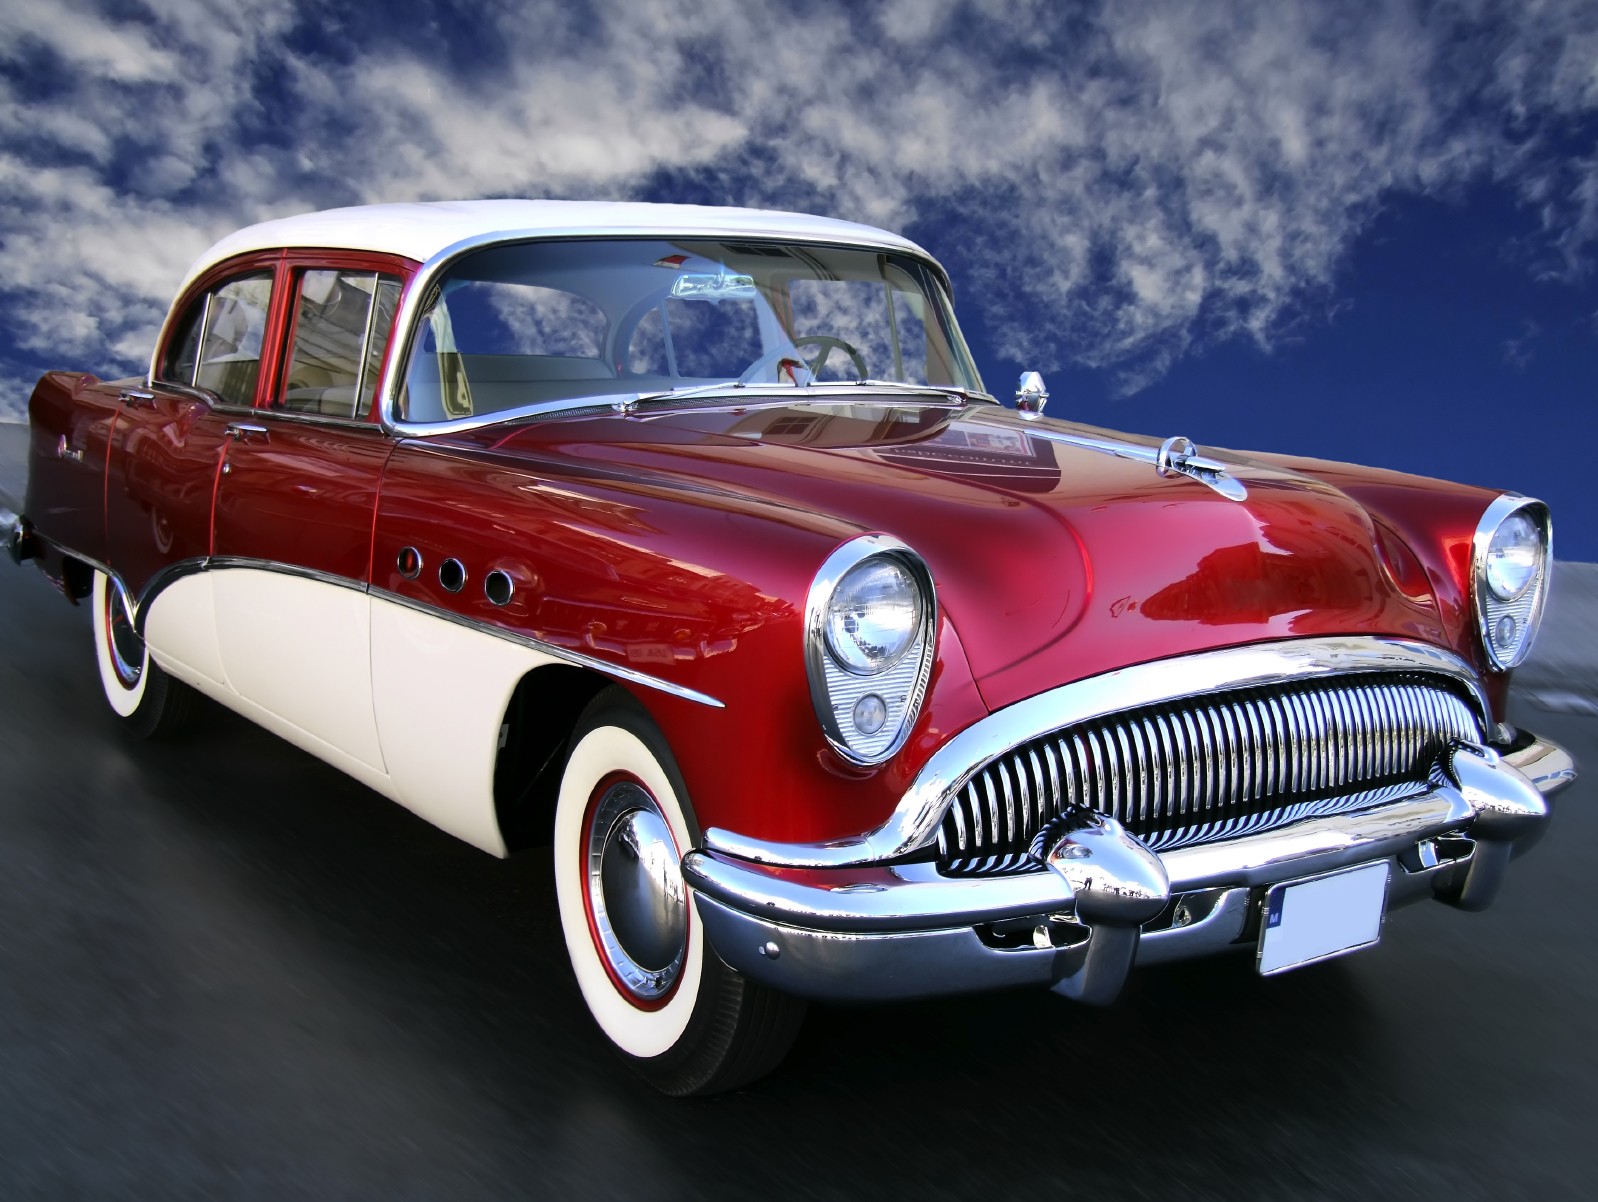
\includegraphics[width=0.4\linewidth]{car.jpg} % original image
		\caption{Original image}
	\end{figure}
\end{center}
%%%%%%%%%%%%%%%%%%%%%%%%%%%%%%%%%%%%%%%%%%
To demonstrate the performance of our trained decoder on the Microsoft COCO dataset \cite{bib10}, we take 5 different images as an input to our encoder-decoder as well as to UST's article encoder-decoder in order to visualize the quality of reconstructed images as presented in figure ~\ref{fig:reconstruction}.\newline
In figure ~\ref{fig:reconstruction} (a) we present Our reconstruction which means the use of trained decoders as in VGG-19 \cite{bib20} and encoder, based on torchvision package.
As can be visually seen, our reconstruction images are less good than Li et al. \cite{bib11} results. Our results suffer from artifacts such as blurring and over smoothing, especially in small details such as faces. This artifacts are outcome of our trained decoder. Section \ref{subsection:decoders} explains why we needed to train 5 different decoders. Without time and compute power limitations we could get much more powerful decoders which are not producing such as artifacts.
In addition, we measure quantitatively (see table ~\ref{Tab:loss}) our reconstruction distortion loss by two measures: pixel loss and feature loss as depicted in equation \ref{eq:loss} and elaborated in \cite{bib22, bib17}.\newline

% ecoder-decoder table %
\begin{center}
	\captionof{table}{Pixel and Feature Loss comparison\label{Tab:loss}}
	\begin{tabular}{ |p{2.5cm}||p{2.5cm}|p{2.5cm}|p{2.5cm}|p{2.5cm}| }
		\hline
		\multicolumn{5}{|c|}{\hspace{1.4cm} Pixel loss \hspace{3cm}$\mid$ \hspace{1cm} Feature loss} \\
		\hline
		architecture &Li et al. \cite{bib11} &Proposed &Li et al. \cite{bib11} &Proposed \\
		\hline
		\centering 1  &.. &..  &.. &..\\
		\hline
		\centering 2 &..  &..   &.. &..\\
		\hline
		\centering 3 &..  &..   &.. &..\\
		\hline
		\centering 4 &..  &..   &.. &..\\
		\hline
		\centering 5 &..  &..   &.. &..\\
		\hline
	\end{tabular}\\
\end{center}
\begin{figure}[H]
% first line
		\centering
	\begin{subfigure}[b]{0.35\linewidth}
		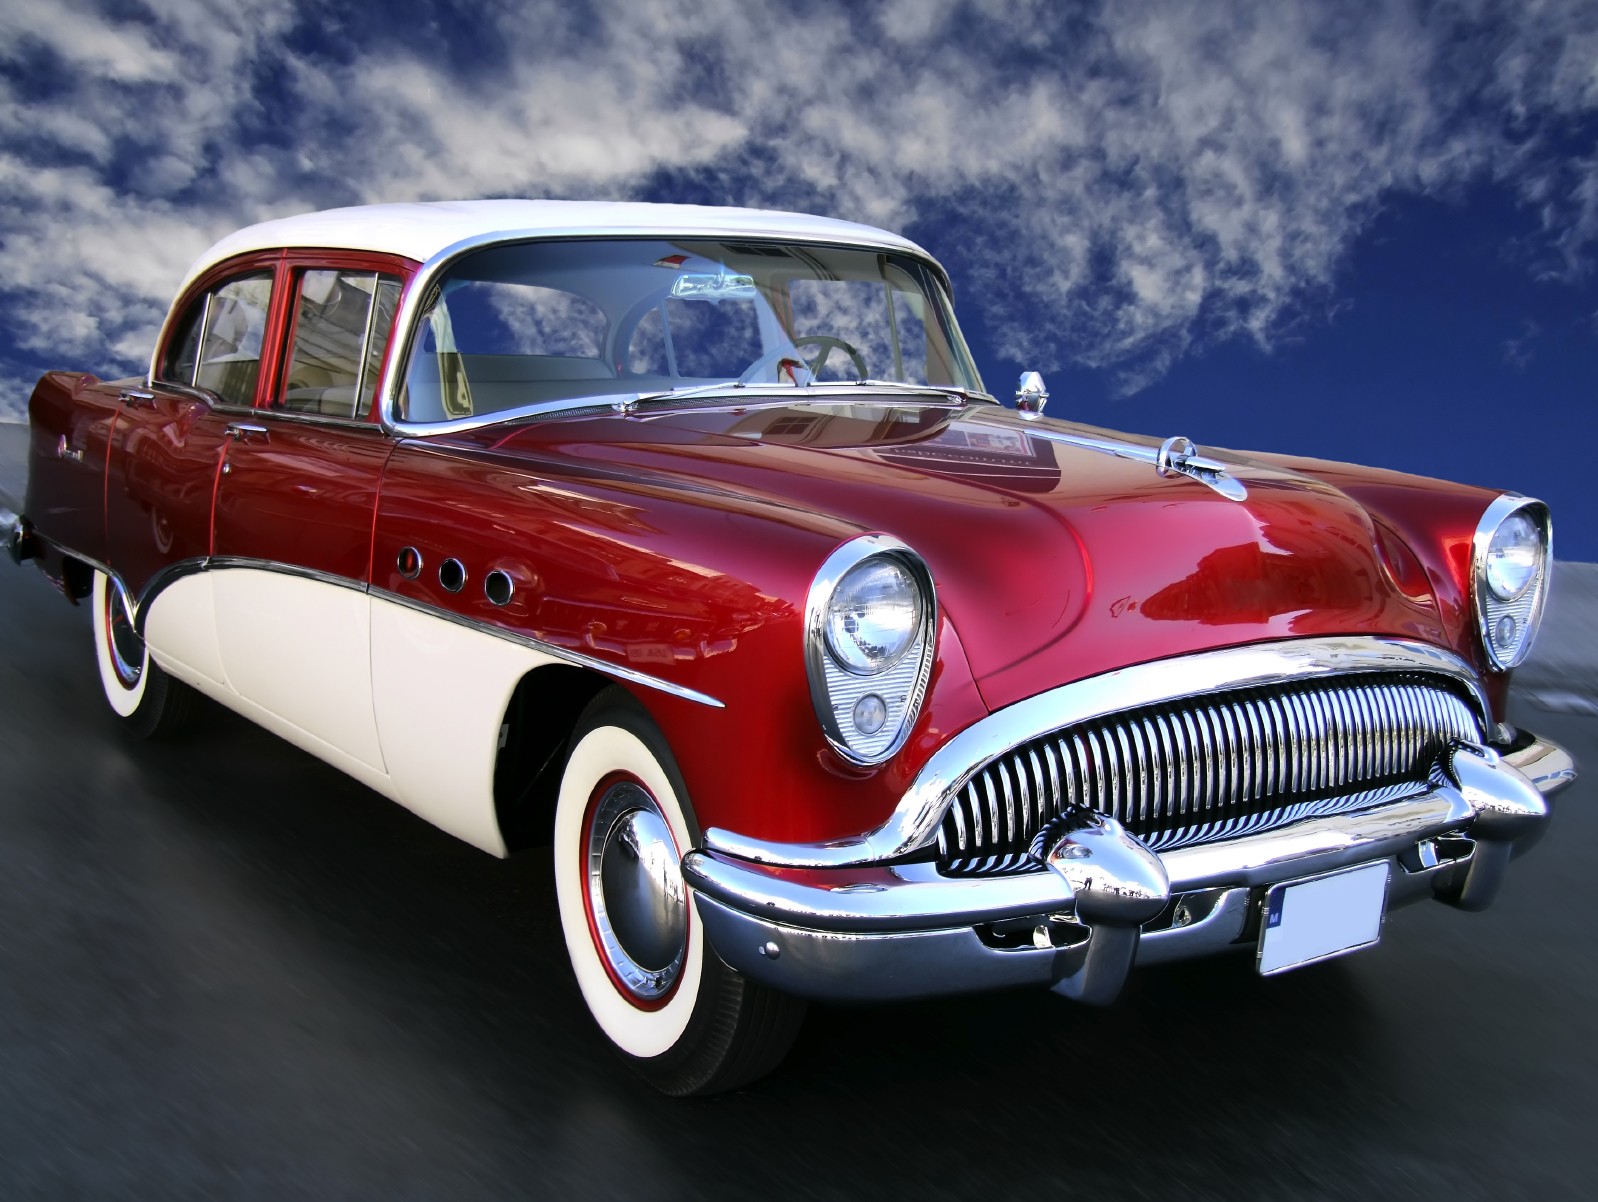
\includegraphics[width=\linewidth]{car.jpg} % our reconstruction num.1	
	\end{subfigure}
	\begin{subfigure}[b]{0.35\linewidth}
		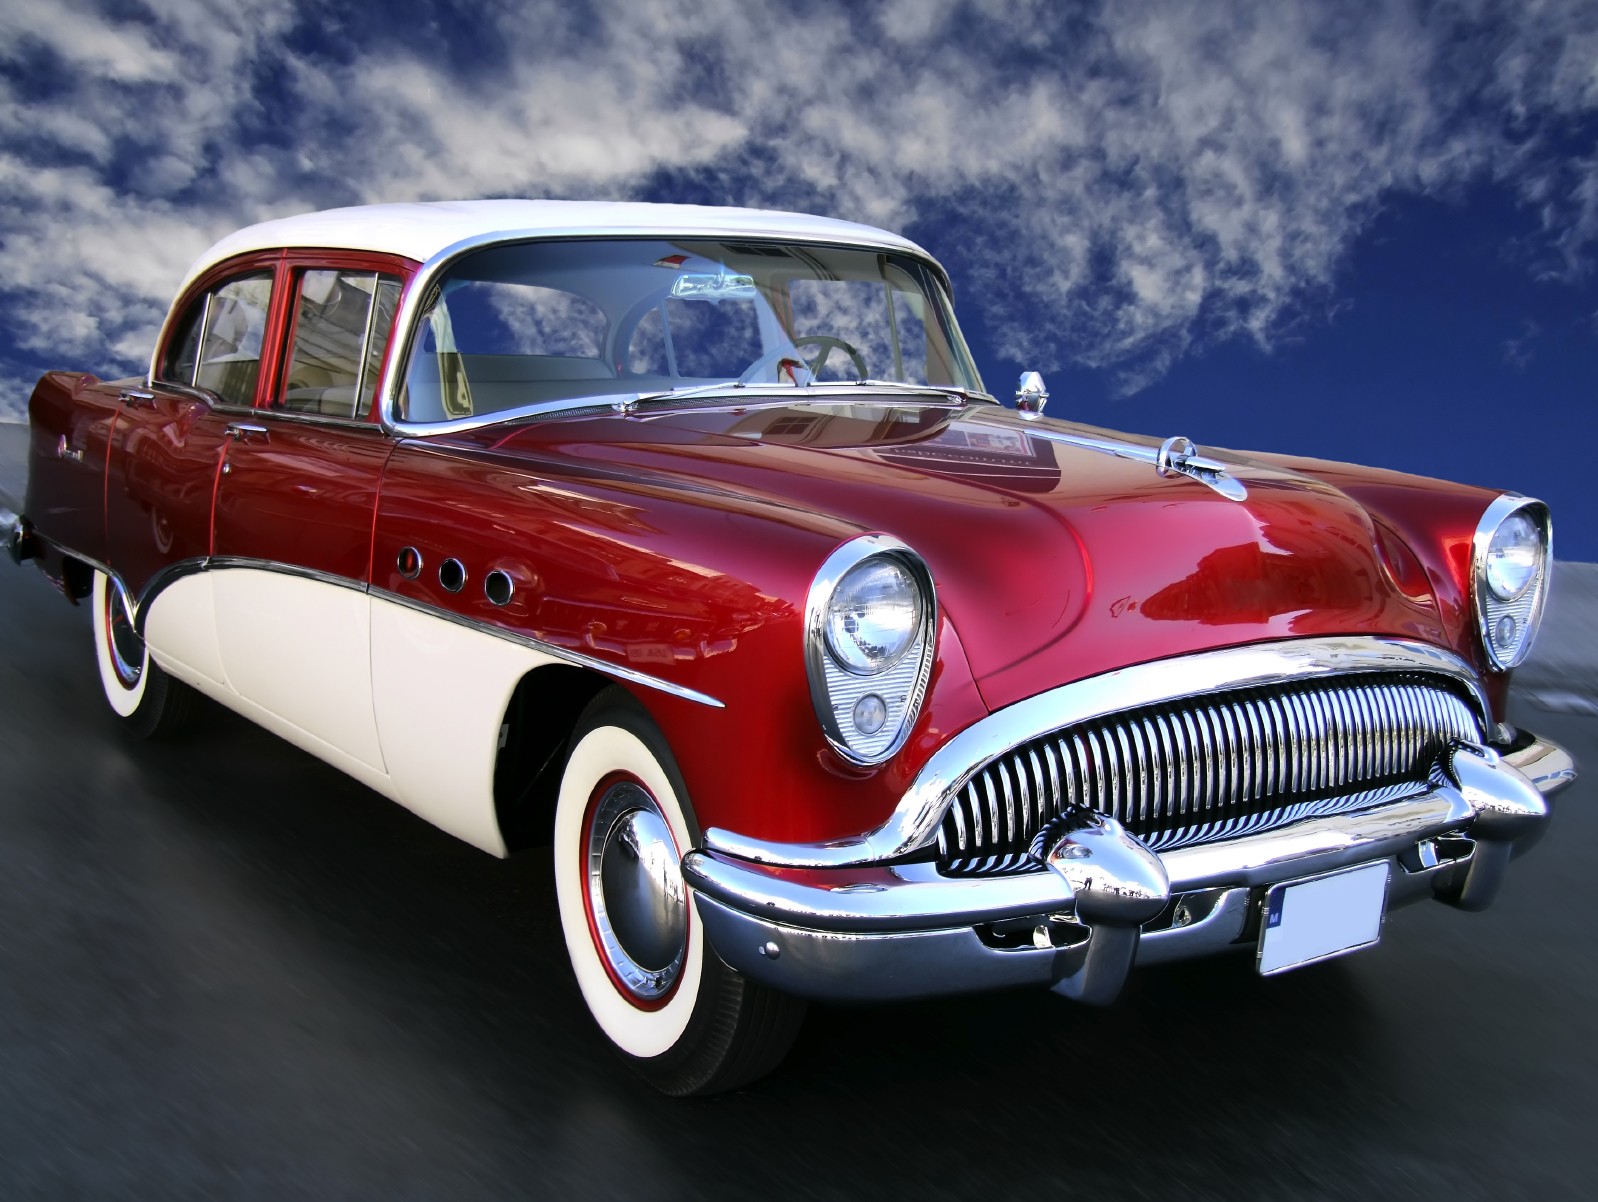
\includegraphics[width=\linewidth]{car.jpg} % their reconstruction num.1	
	\end{subfigure}
% second line
		\centering
	\begin{subfigure}[b]{0.35\linewidth}
		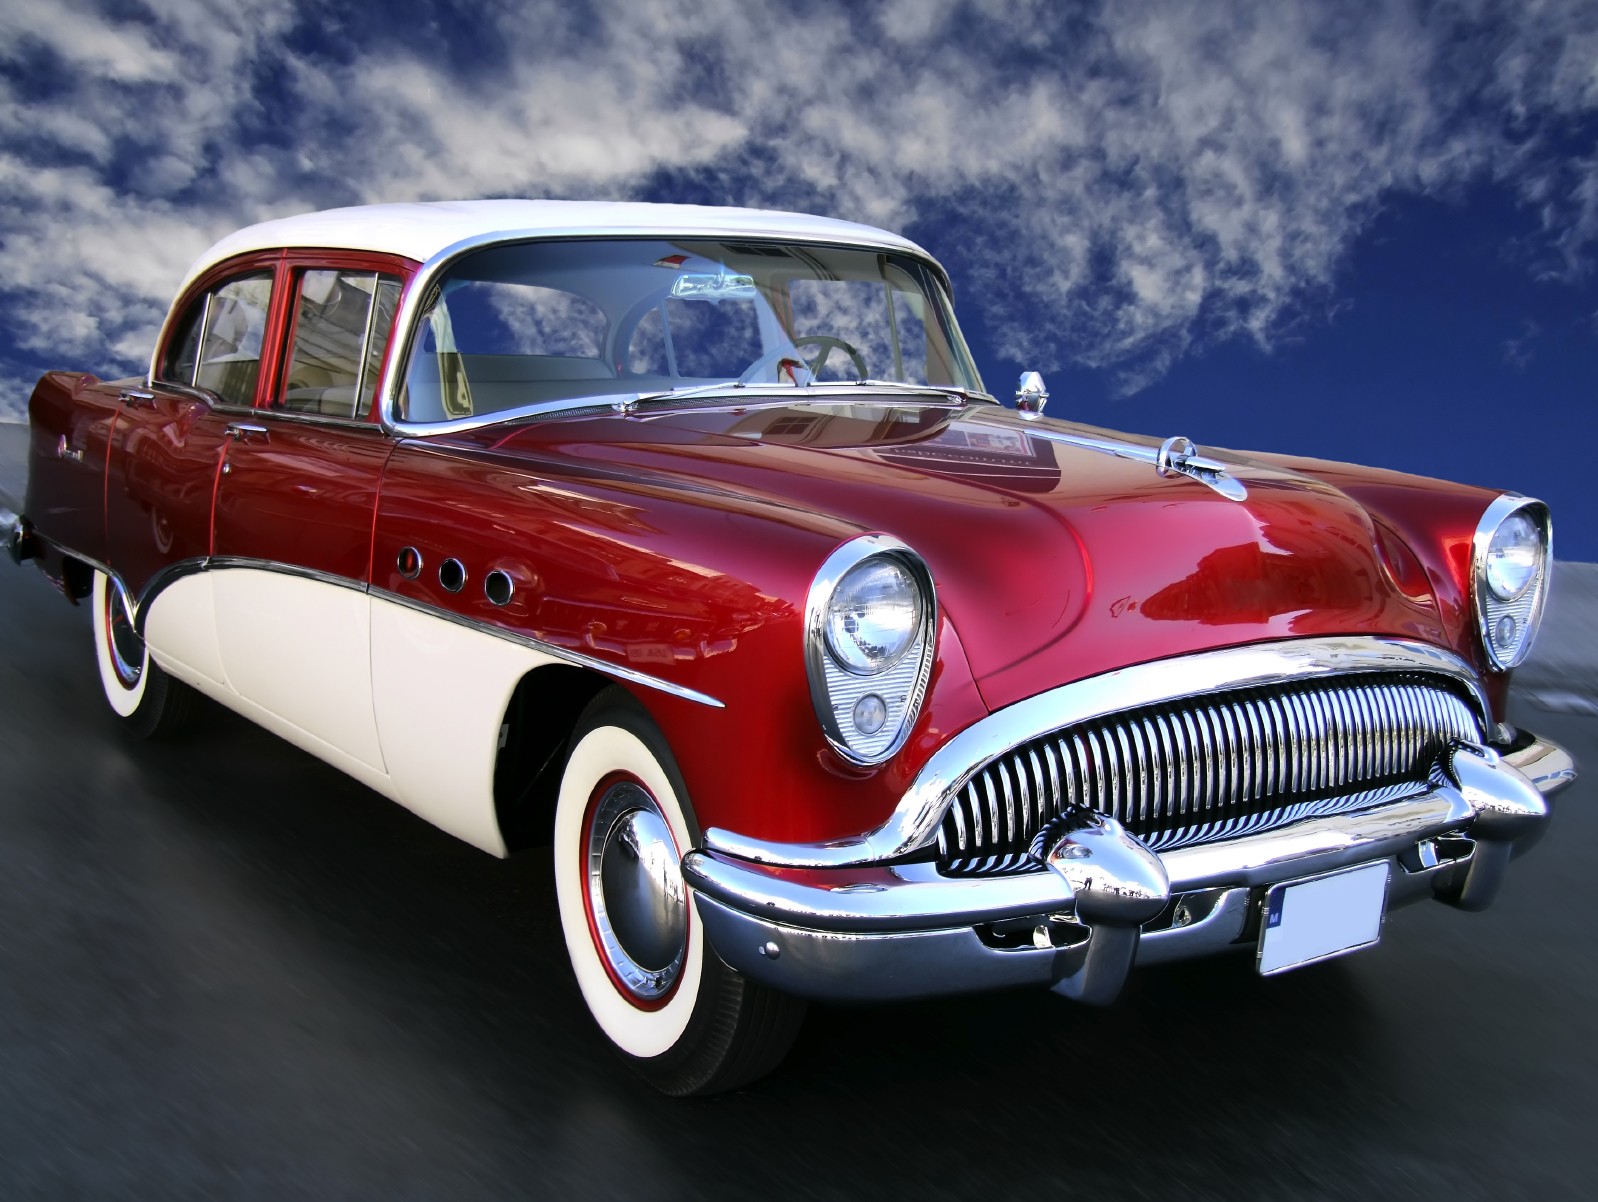
\includegraphics[width=\linewidth]{car.jpg} % our reconstruction num.2
	\end{subfigure}
	\begin{subfigure}[b]{0.35\linewidth}
		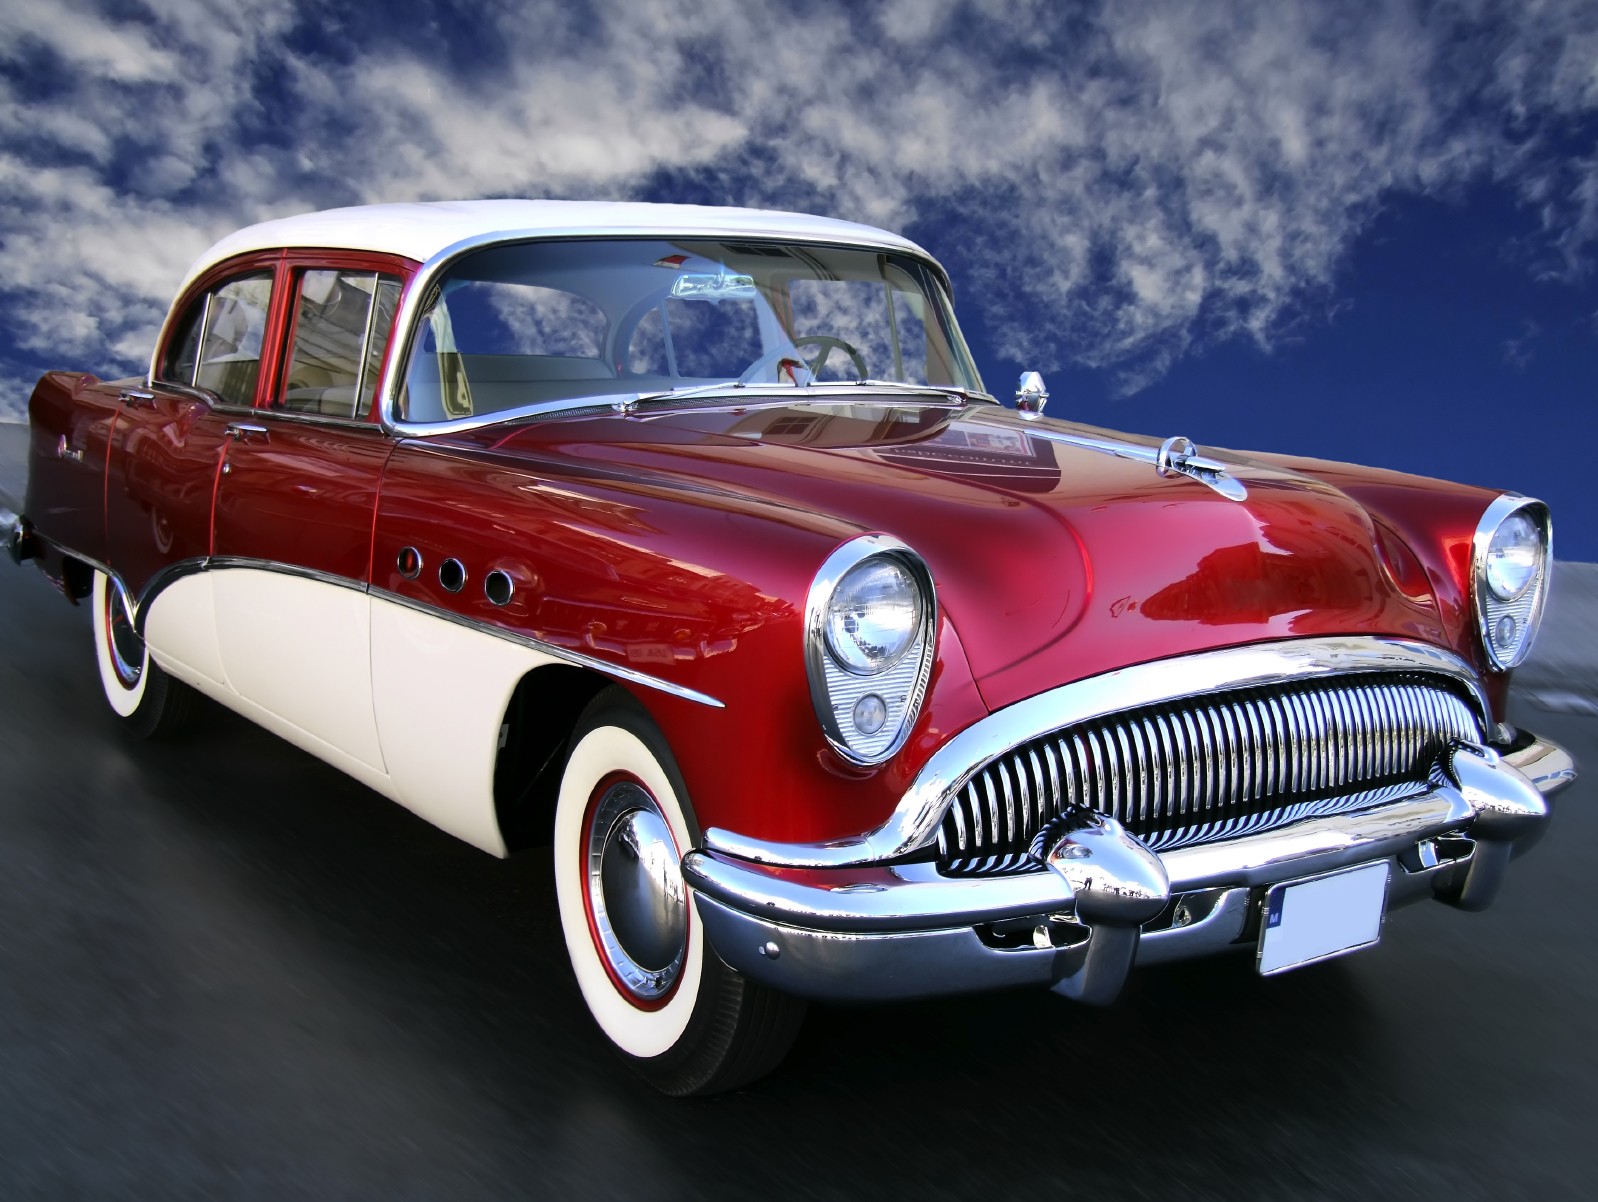
\includegraphics[width=\linewidth]{car.jpg} % their reconstruction num.2
	\end{subfigure}
% third line
		\centering
	\begin{subfigure}[b]{0.35\linewidth}
		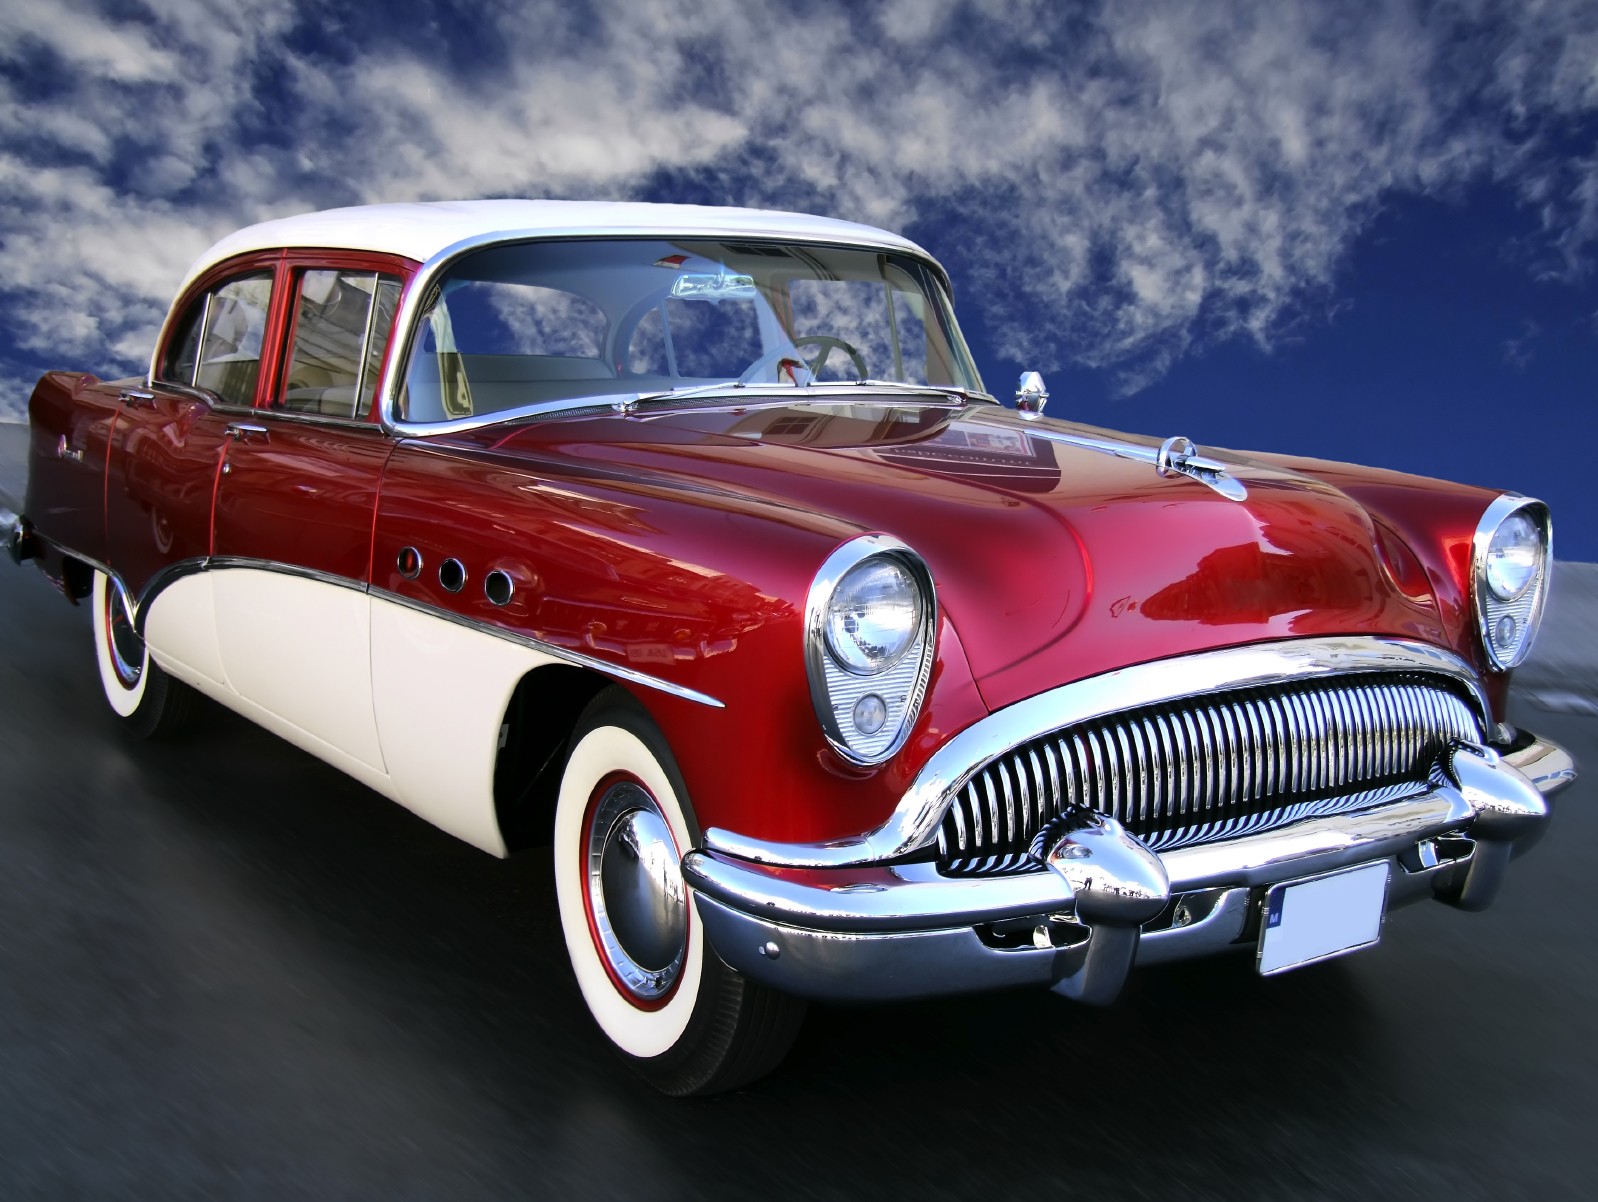
\includegraphics[width=\linewidth]{car.jpg} % our reconstruction num.3
	\end{subfigure}
	\begin{subfigure}[b]{0.35\linewidth}
		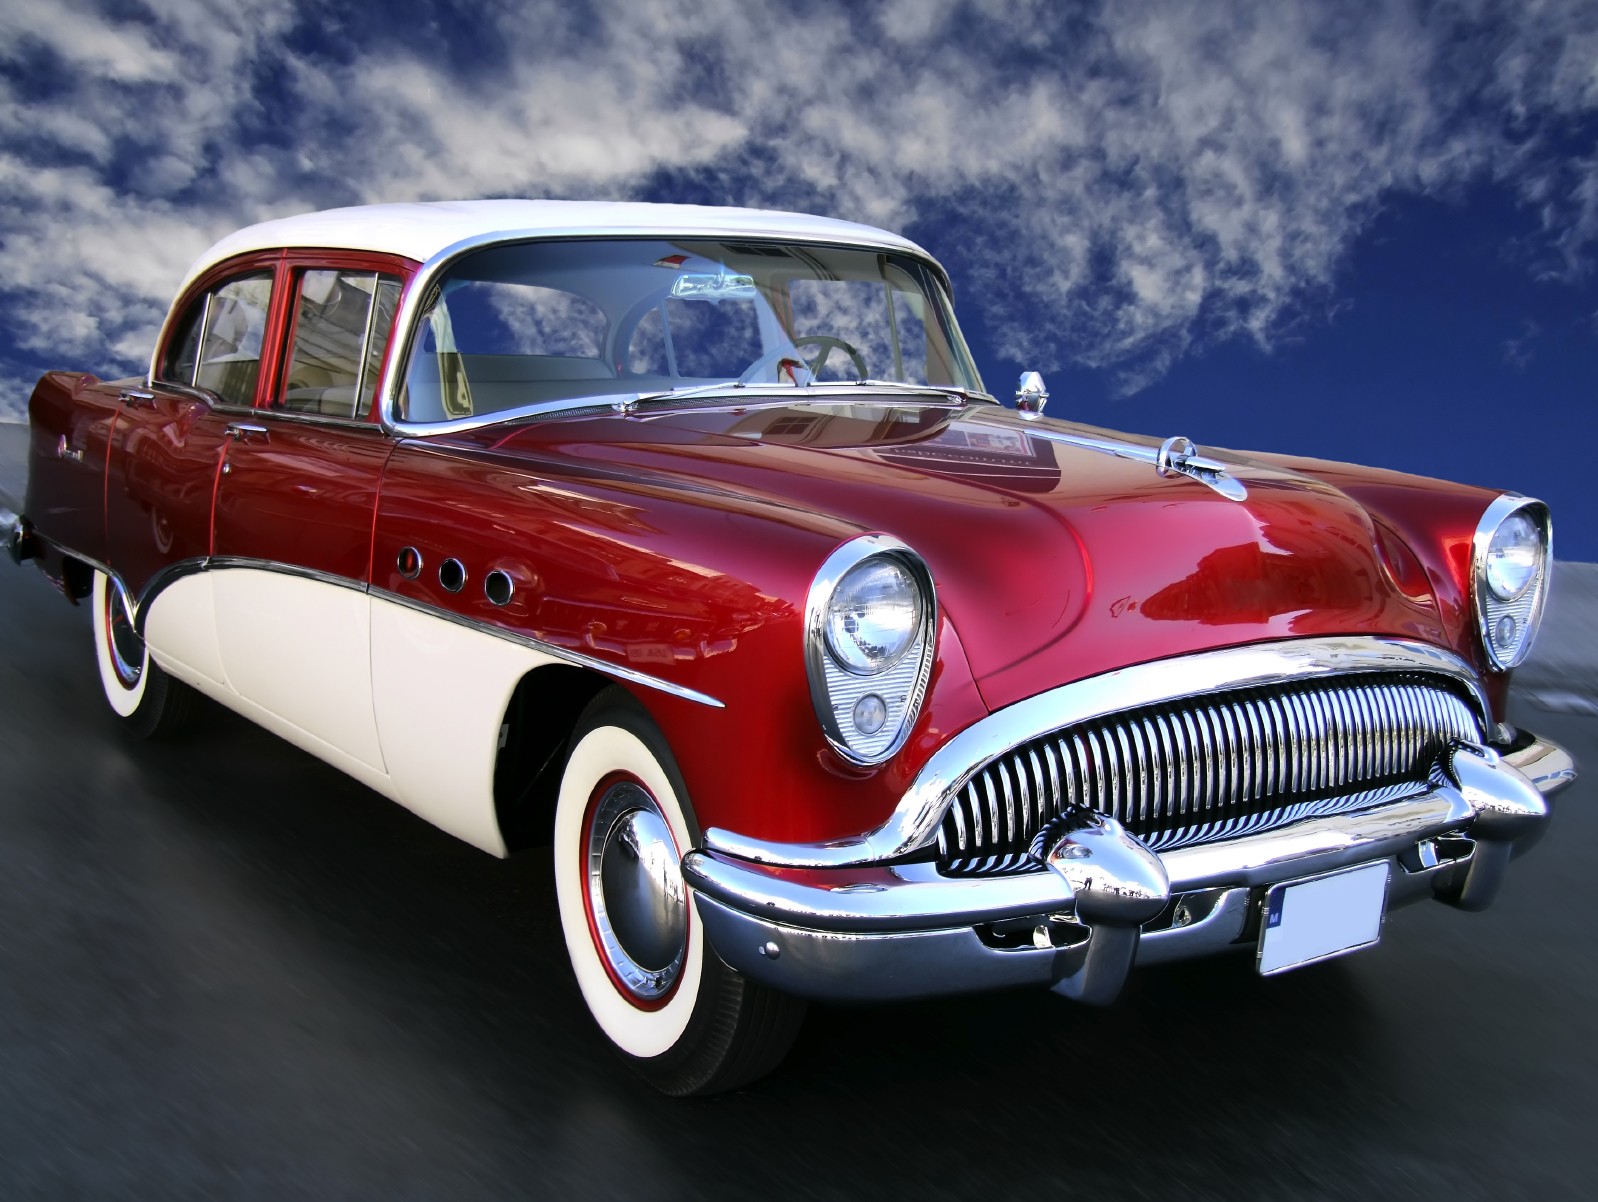
\includegraphics[width=\linewidth]{car.jpg} % their reconstruction num.3
	\end{subfigure}
% fourth line
	\centering
	\begin{subfigure}[b]{0.35\linewidth}
		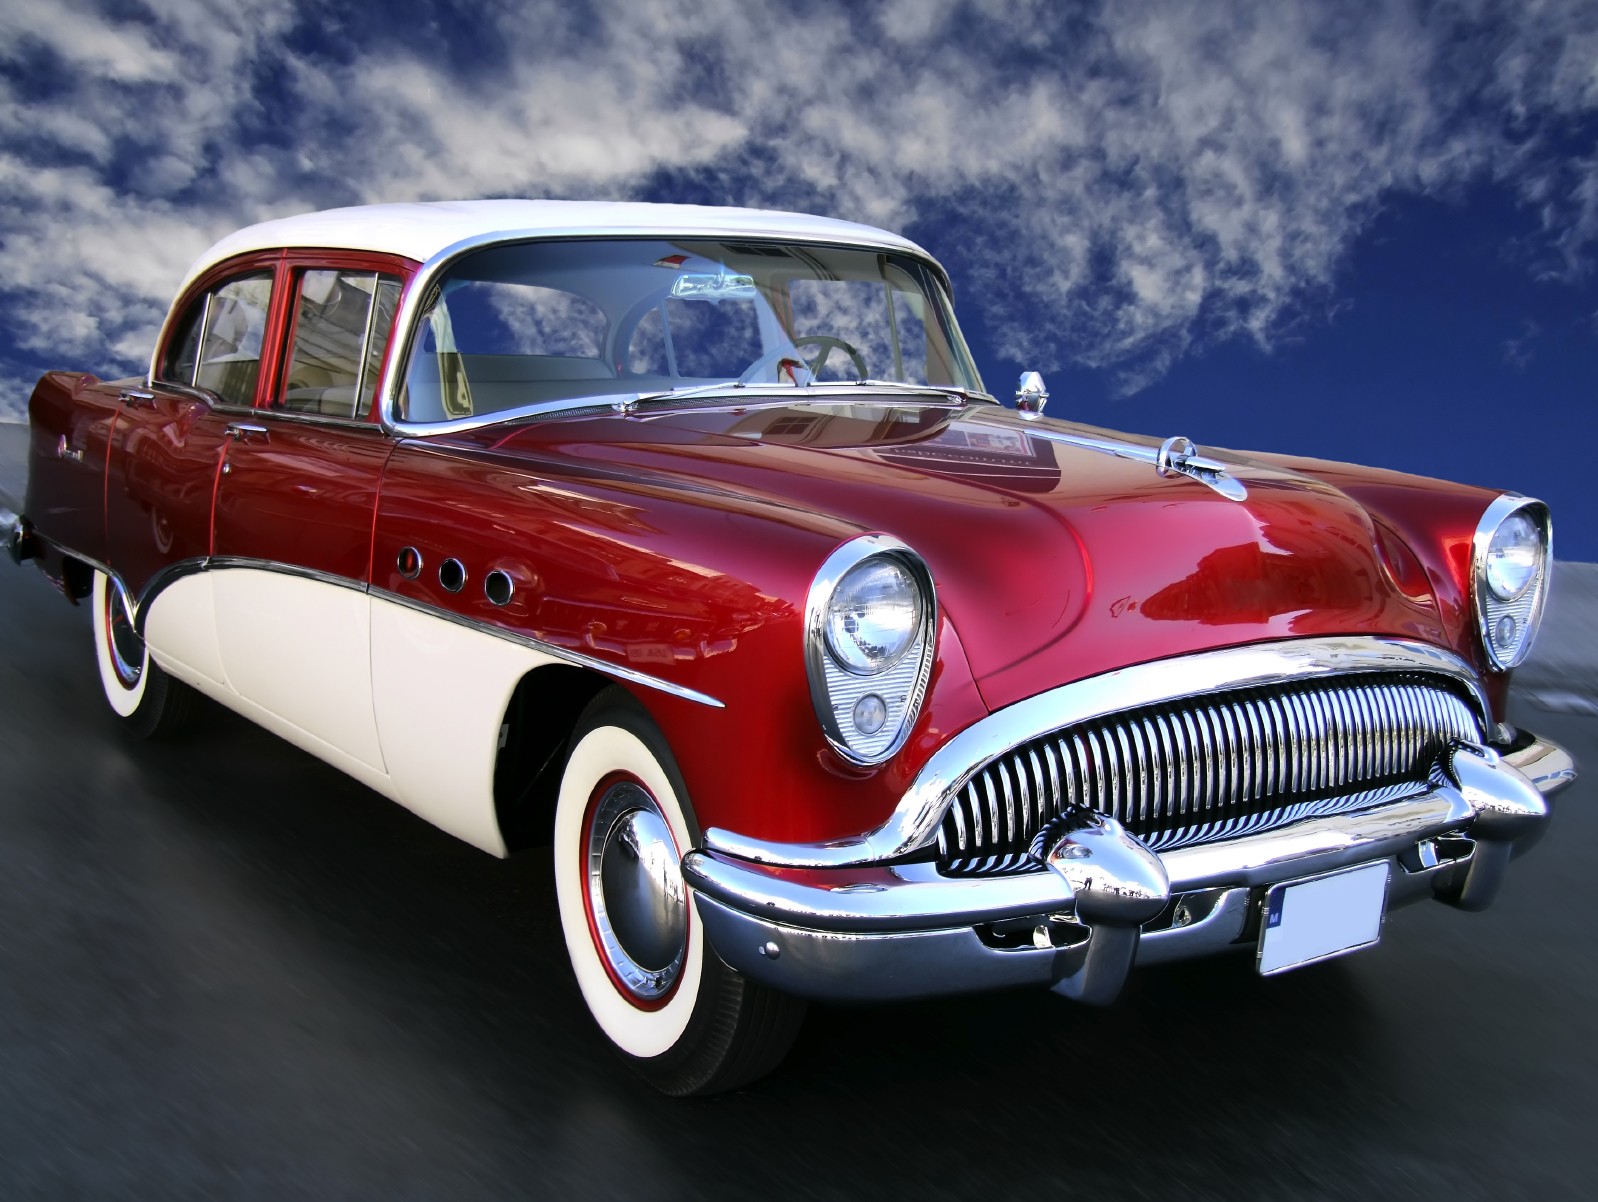
\includegraphics[width=\linewidth]{car.jpg} % our reconstruction num.4
	\end{subfigure}
	\begin{subfigure}[b]{0.35\linewidth}
		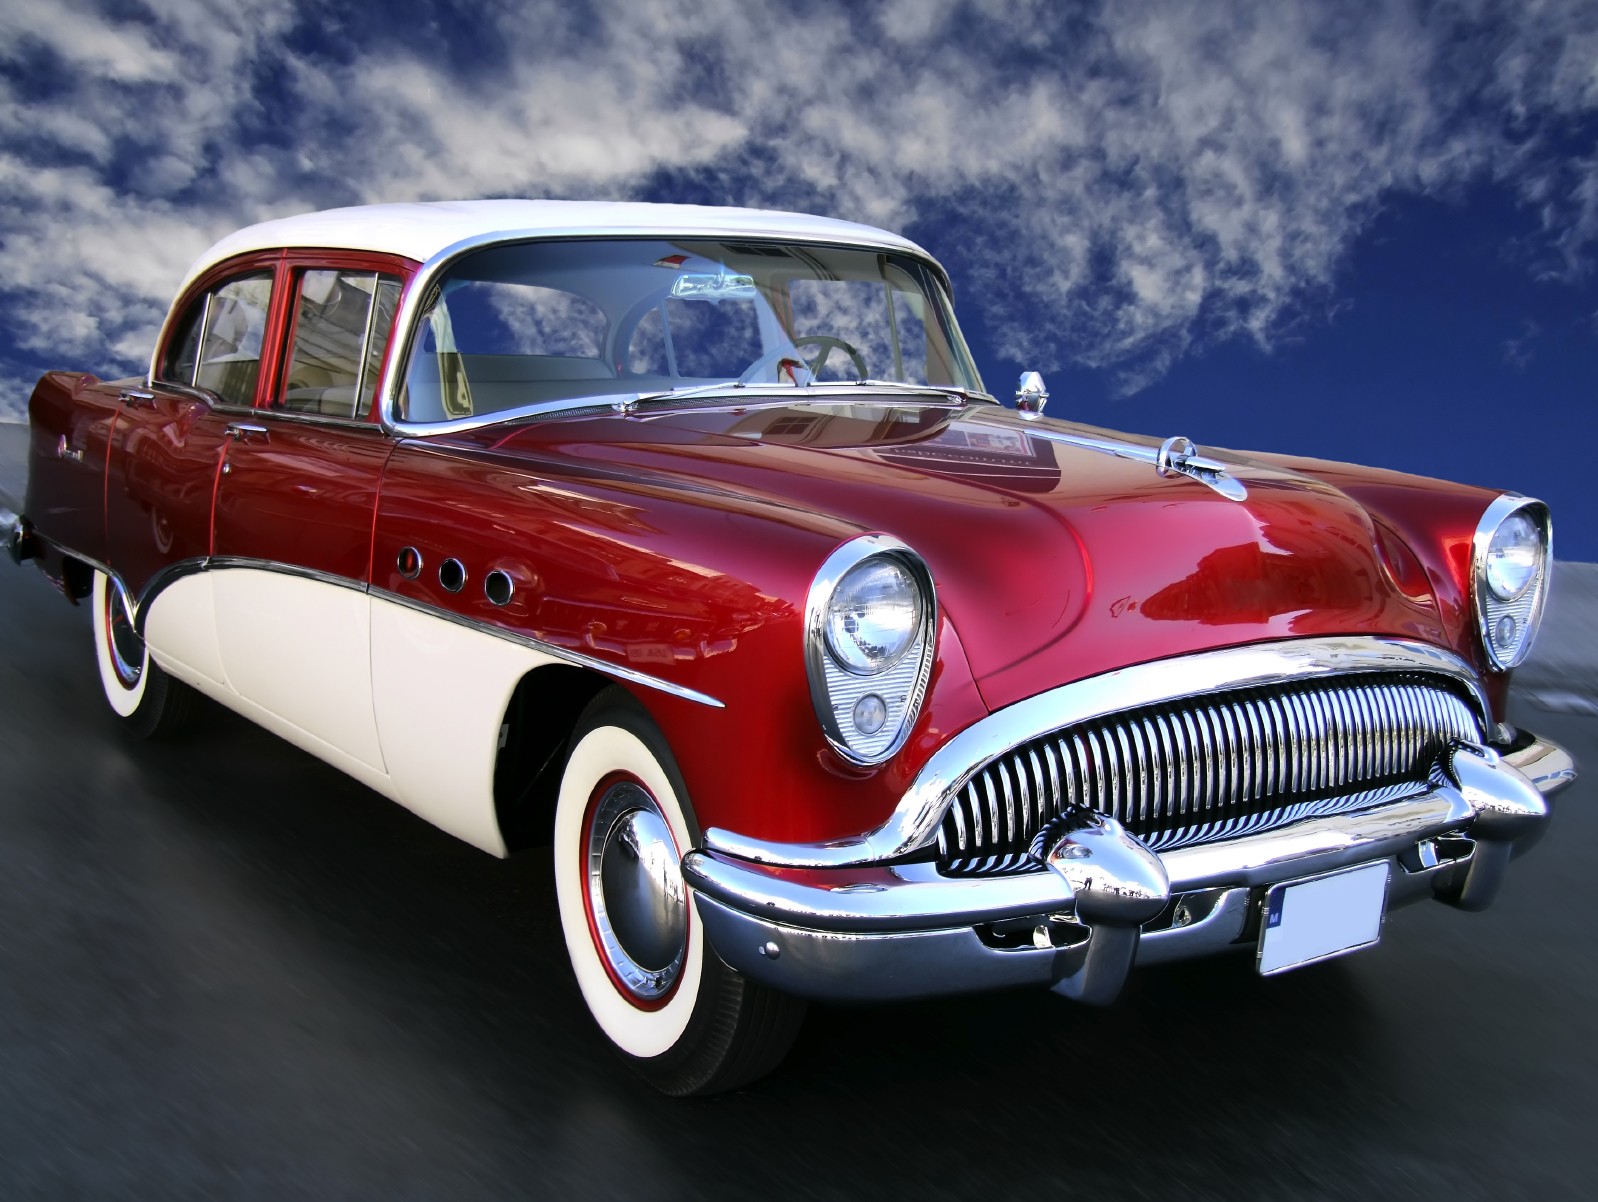
\includegraphics[width=\linewidth]{car.jpg} % their reconstruction num.4
	\end{subfigure}
% fifth line
		\centering
	\begin{subfigure}[b]{0.35\linewidth}
		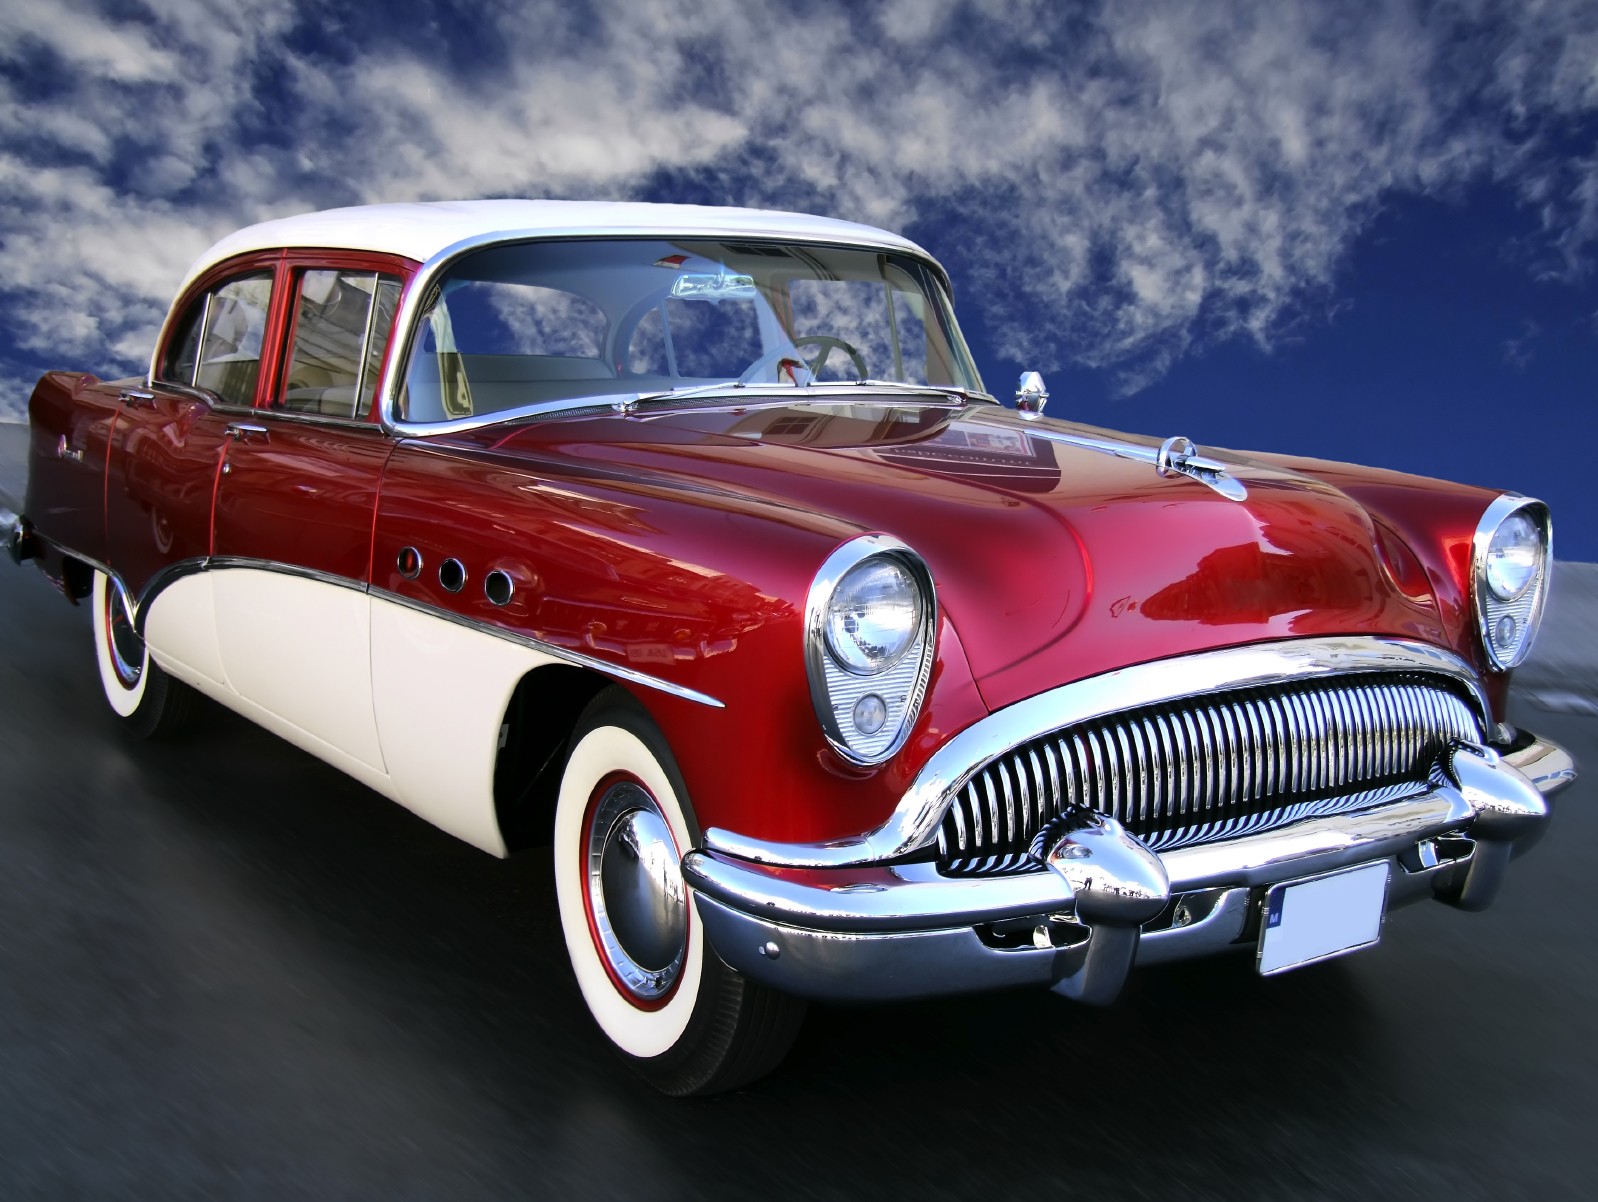
\includegraphics[width=\linewidth]{car.jpg} % our reconstruction num.5
		\caption{Our reconstruction}
	\end{subfigure}
	\begin{subfigure}[b]{0.35\linewidth}
		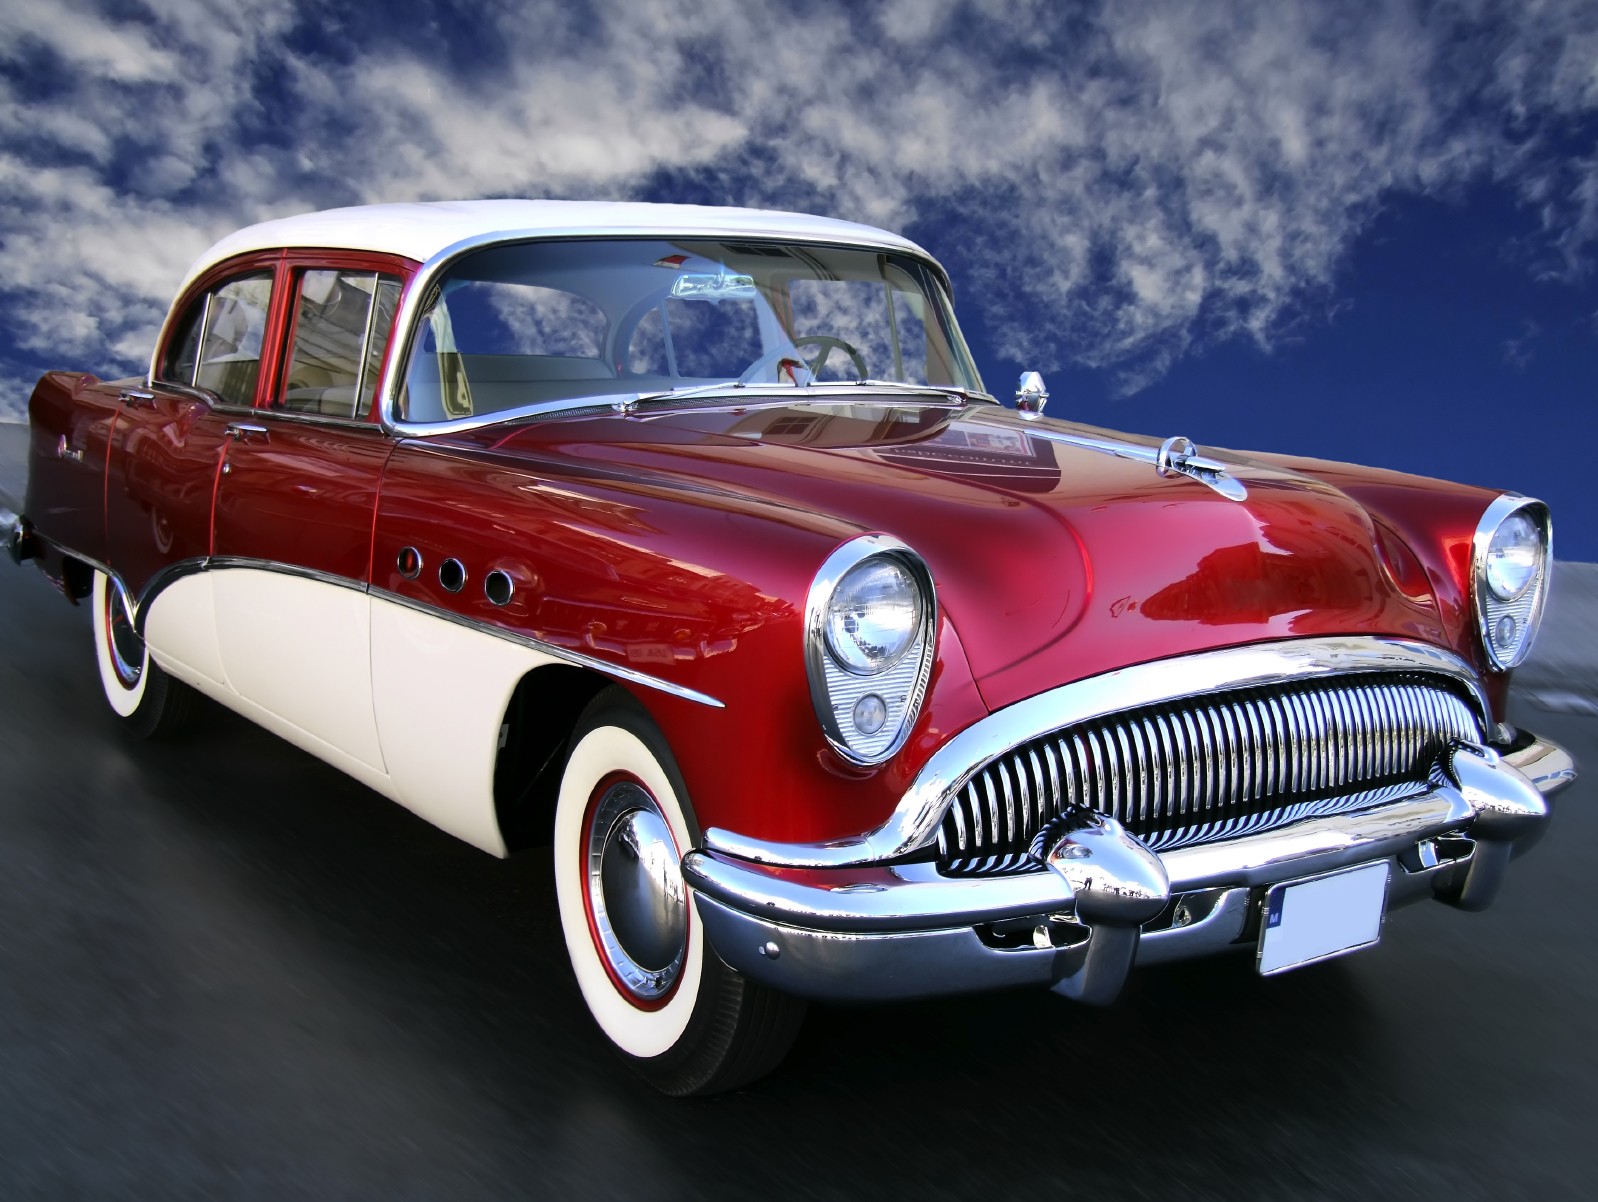
\includegraphics[width=\linewidth]{car.jpg} % their reconstruction num.5
		\caption{Li et al. \cite{bib11}}	
	\end{subfigure}
	\caption{Reconstructed images}
	\label{fig:reconstruction}
\end{figure}
  
%%%%%%%%%%%%%%%%%%%%%%%%%%%%
%%%%%%%%%%%%%%%%%%%%%%%%%%%%
% style transfer images %
%%%%%%%%%%%%%%%%%%%%%%%%%%%%
%%%%%%%%%%%%%%%%%%%%%%%%%%%%
\subsection{style transfer}
\begin{figure}[H]
	% first line
	\centering
	\begin{subfigure}[b]{0.225\linewidth}
		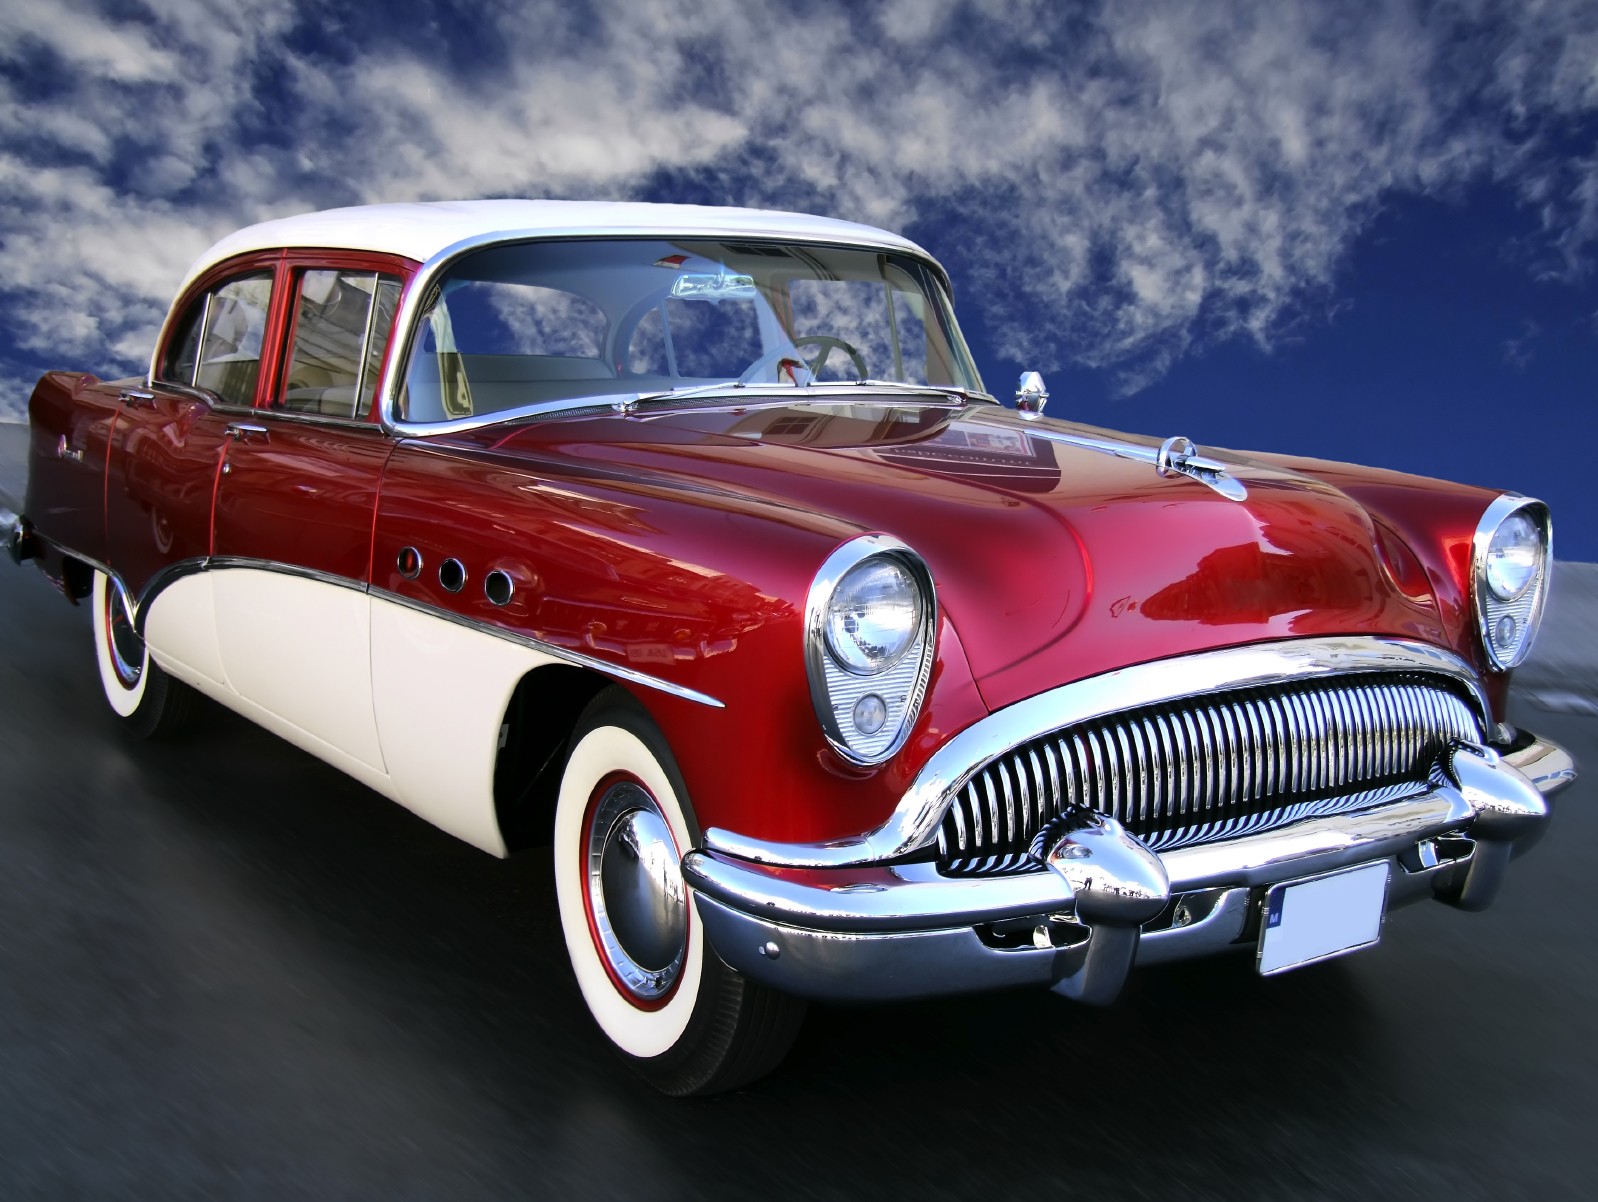
\includegraphics[width=\linewidth]{car.jpg} % style img num.1
	\end{subfigure}
	\begin{subfigure}[b]{0.225\linewidth}
		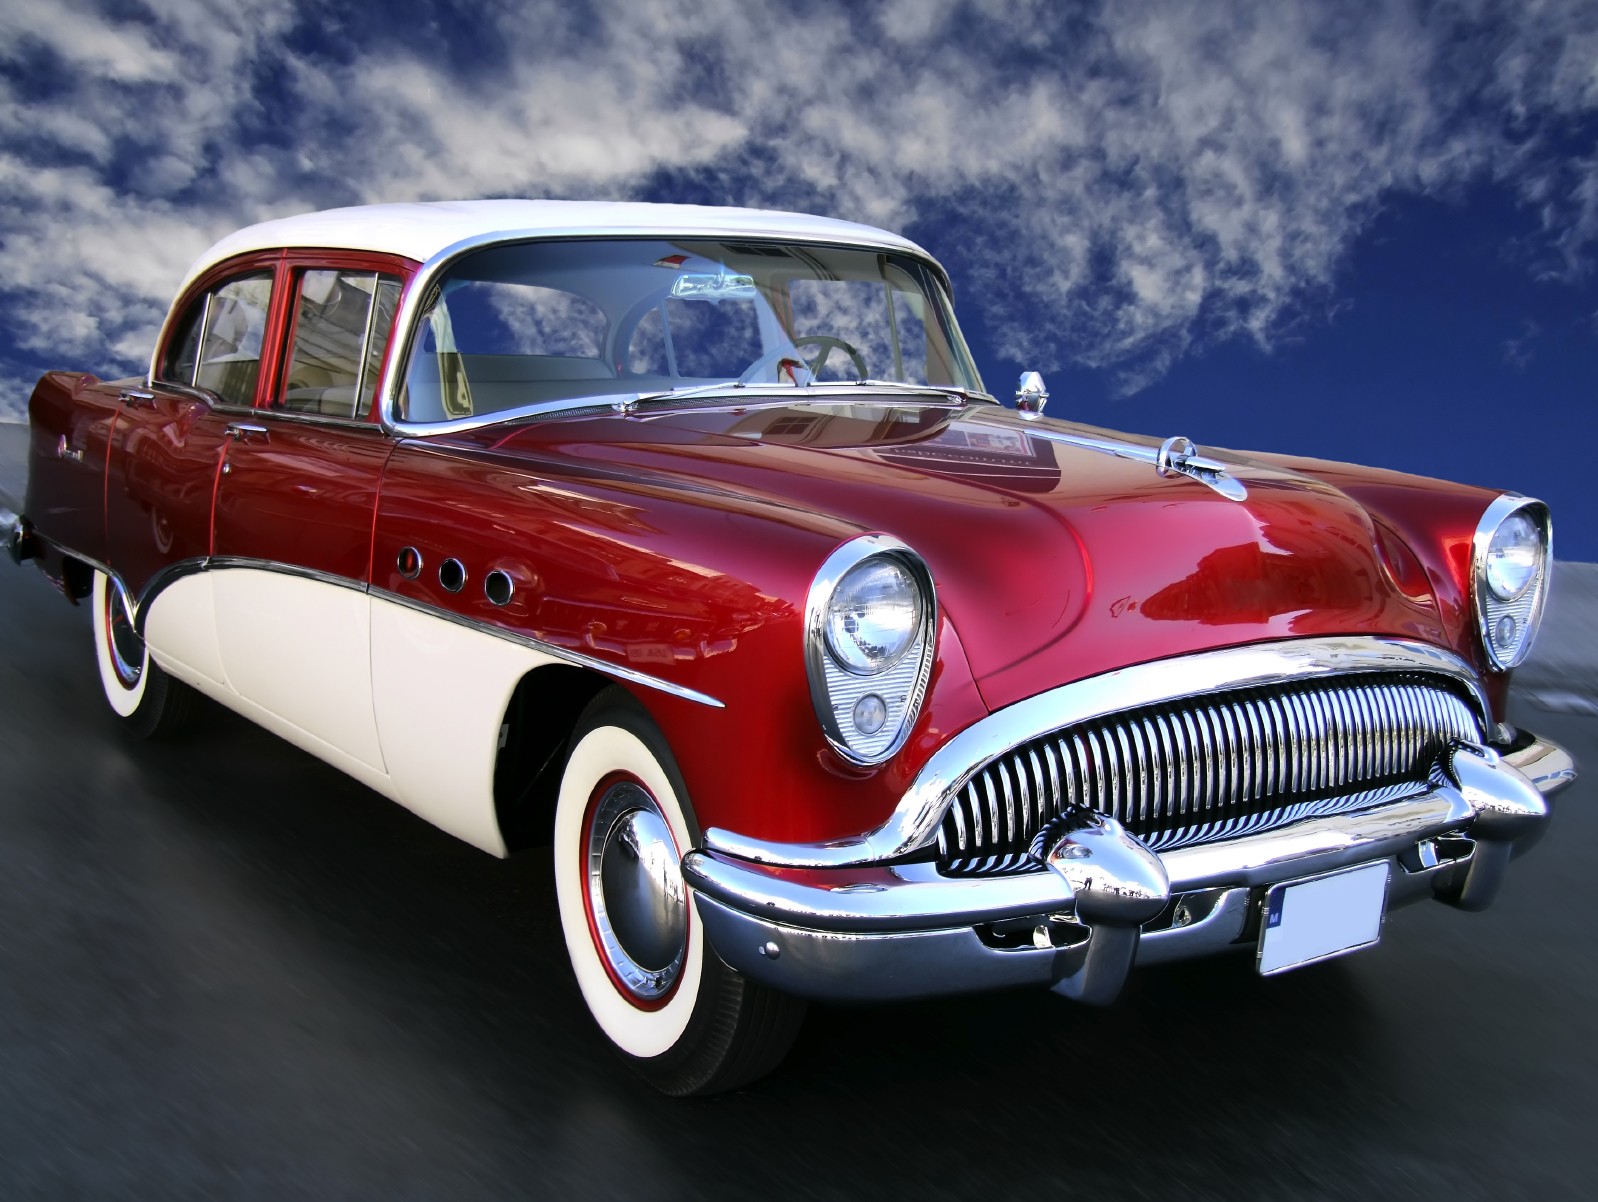
\includegraphics[width=\linewidth]{car.jpg} % content img num.1	
	\end{subfigure}
	\begin{subfigure}[b]{0.225\linewidth}
		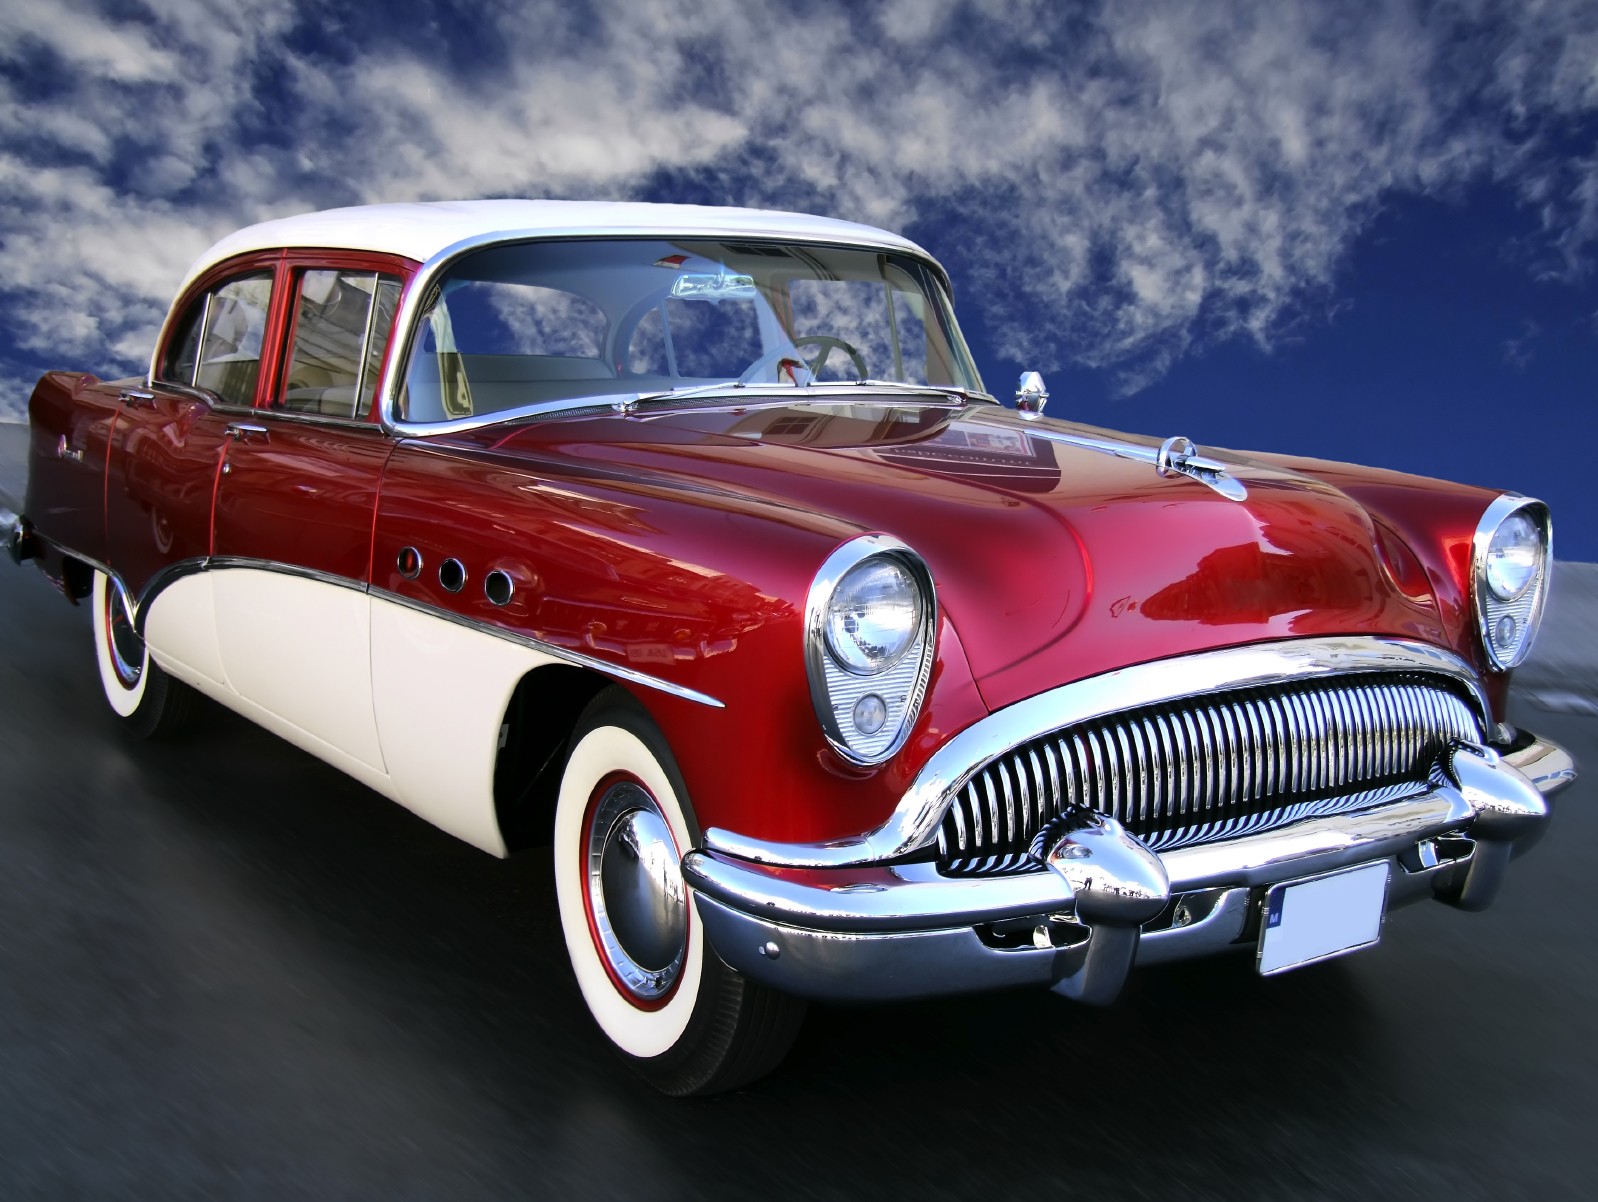
\includegraphics[width=\linewidth]{car.jpg} % theirs reconstruction num.1	
	\end{subfigure}
	\begin{subfigure}[b]{0.225\linewidth}
		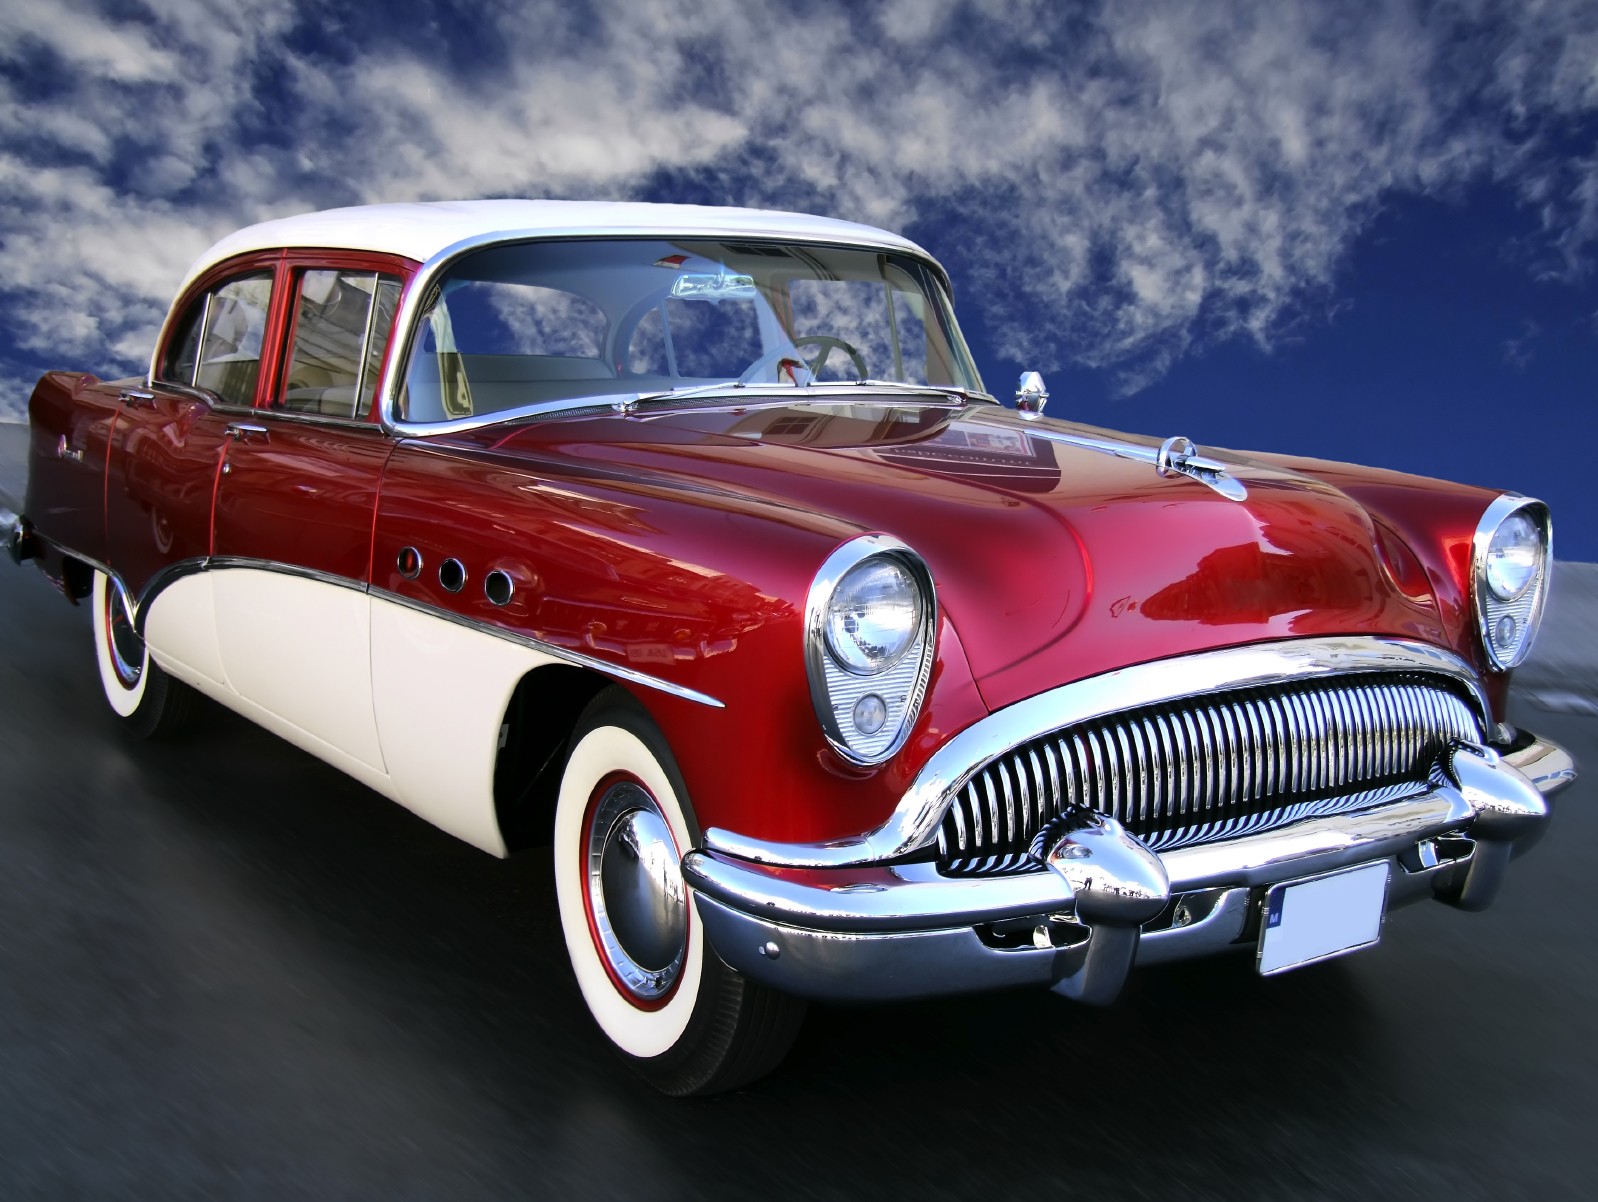
\includegraphics[width=\linewidth]{car.jpg} % ours reconstruction num.1	
	\end{subfigure}
	% second line
	\centering
	\begin{subfigure}[b]{0.225\linewidth}
		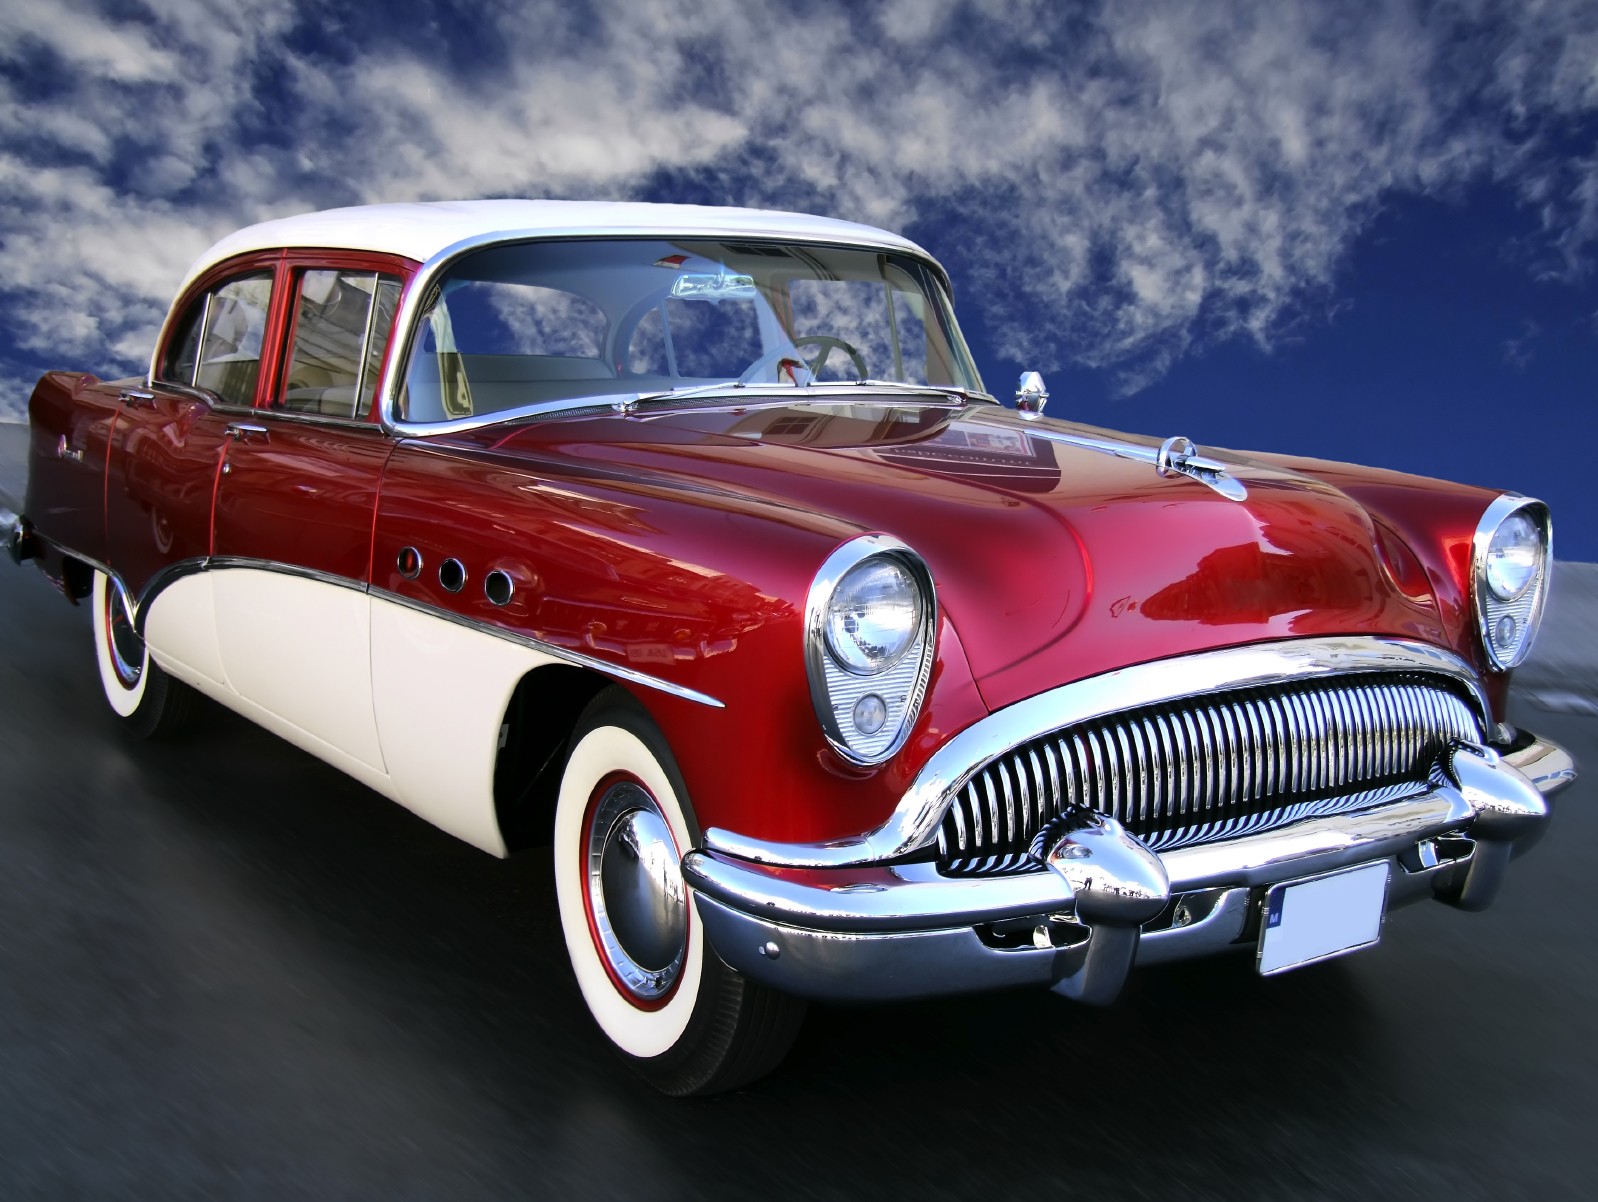
\includegraphics[width=\linewidth]{car.jpg} %style img num.2
	\end{subfigure}
	\begin{subfigure}[b]{0.225\linewidth}
		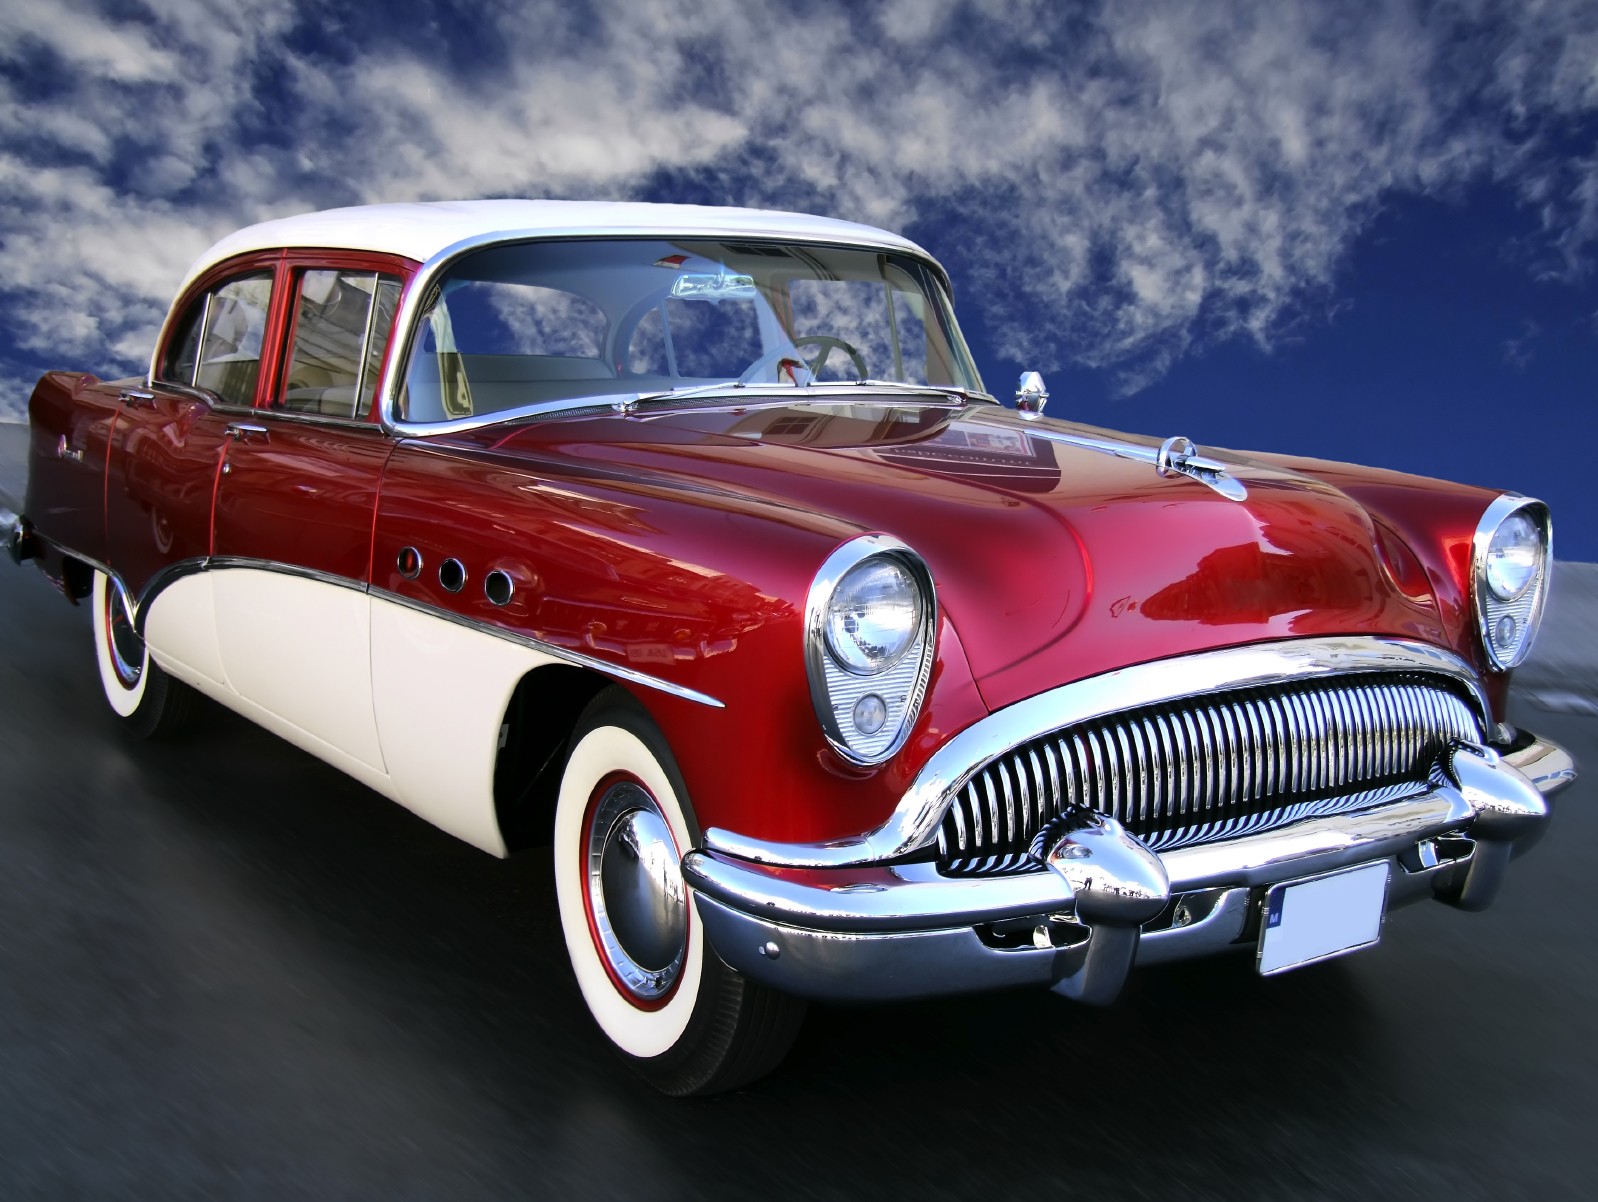
\includegraphics[width=\linewidth]{car.jpg} % content img num.2
	\end{subfigure}
	\begin{subfigure}[b]{0.225\linewidth}
		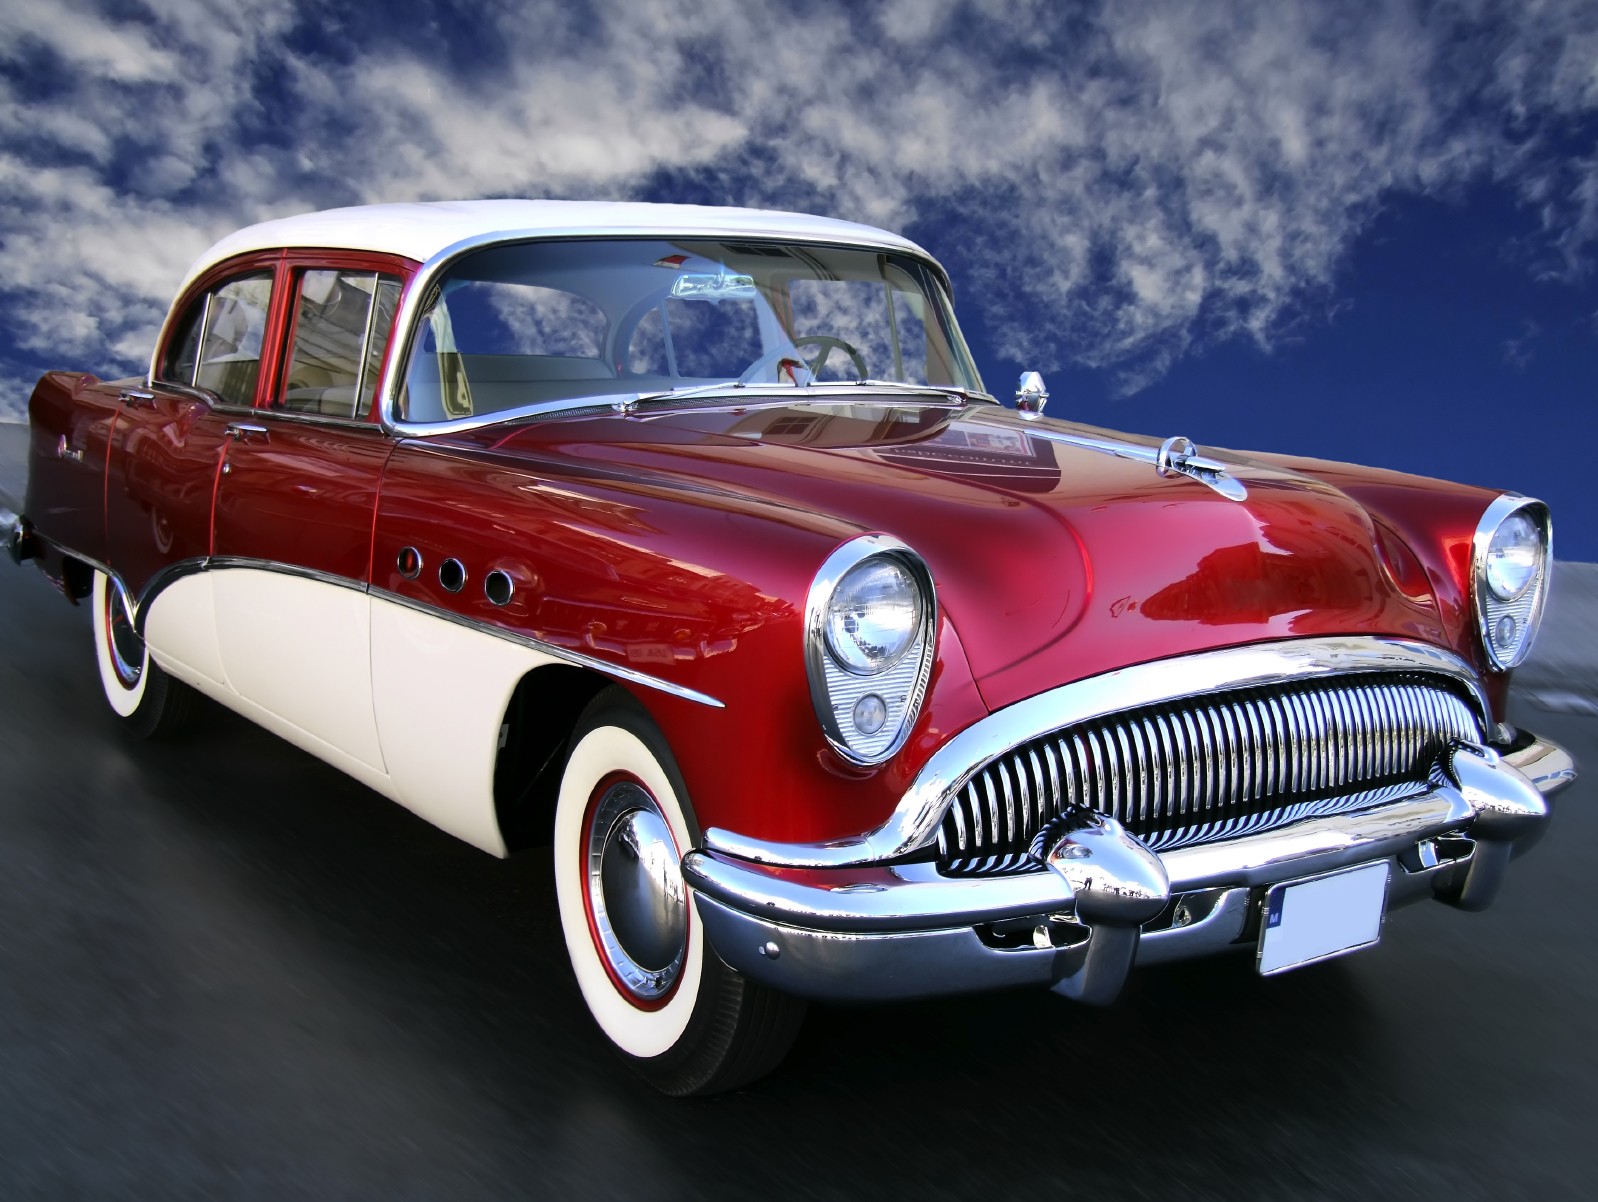
\includegraphics[width=\linewidth]{car.jpg} % theirs reconstruction num.2
	\end{subfigure}
	\begin{subfigure}[b]{0.225\linewidth}
		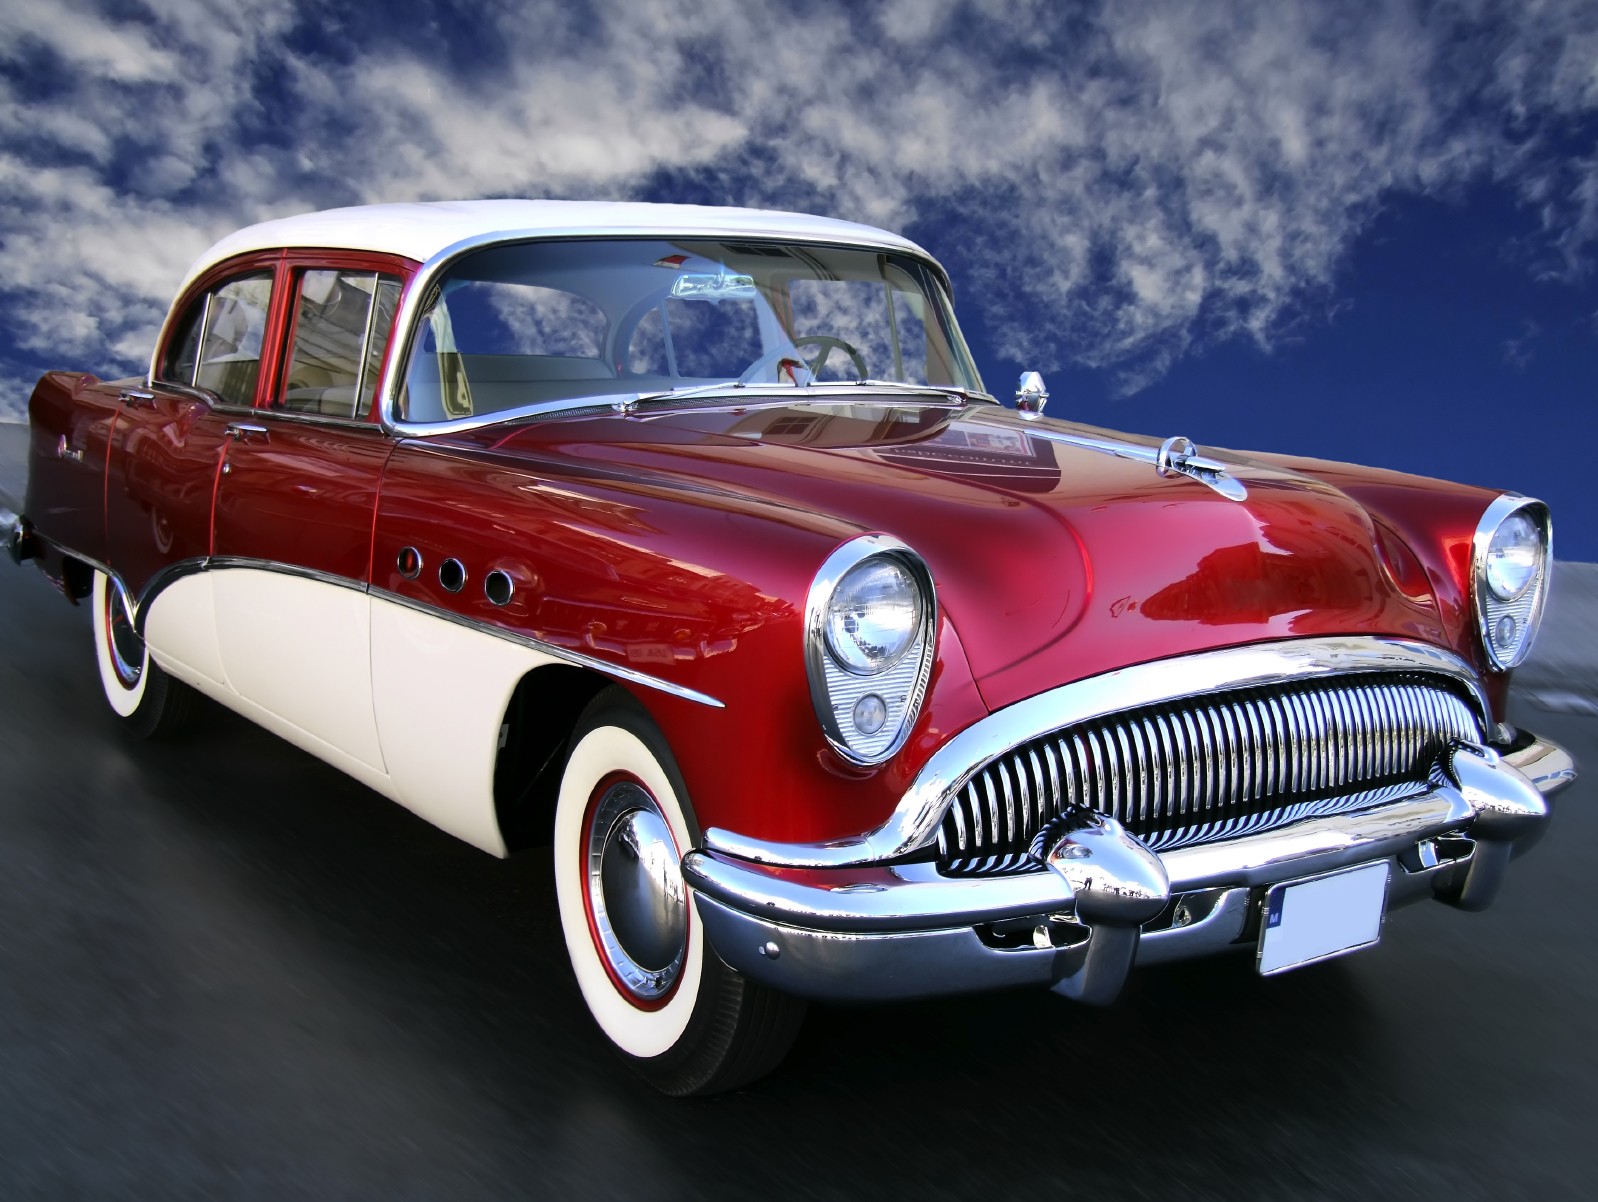
\includegraphics[width=\linewidth]{car.jpg} % ours reconstruction num.2
	\end{subfigure}
	% third line
	\centering
	\begin{subfigure}[b]{0.225\linewidth}
		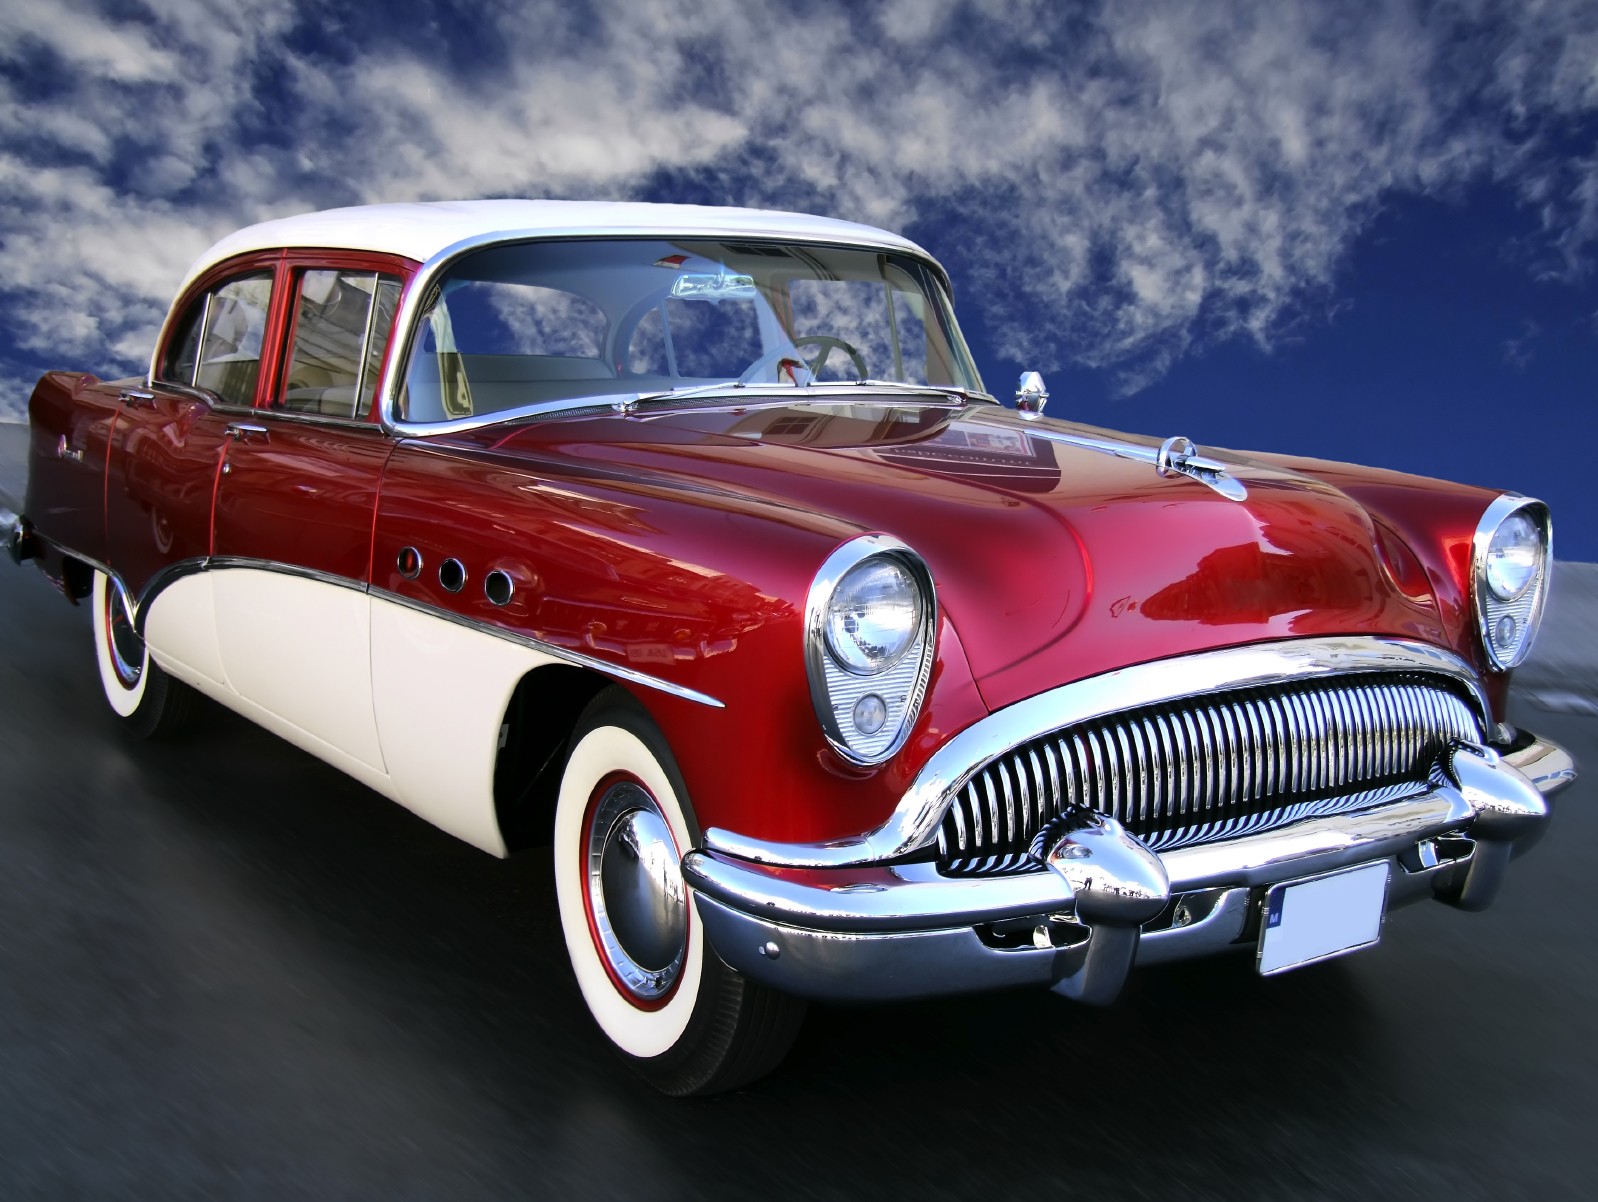
\includegraphics[width=\linewidth]{car.jpg} %style img num.3
	\end{subfigure}
	\begin{subfigure}[b]{0.225\linewidth}
		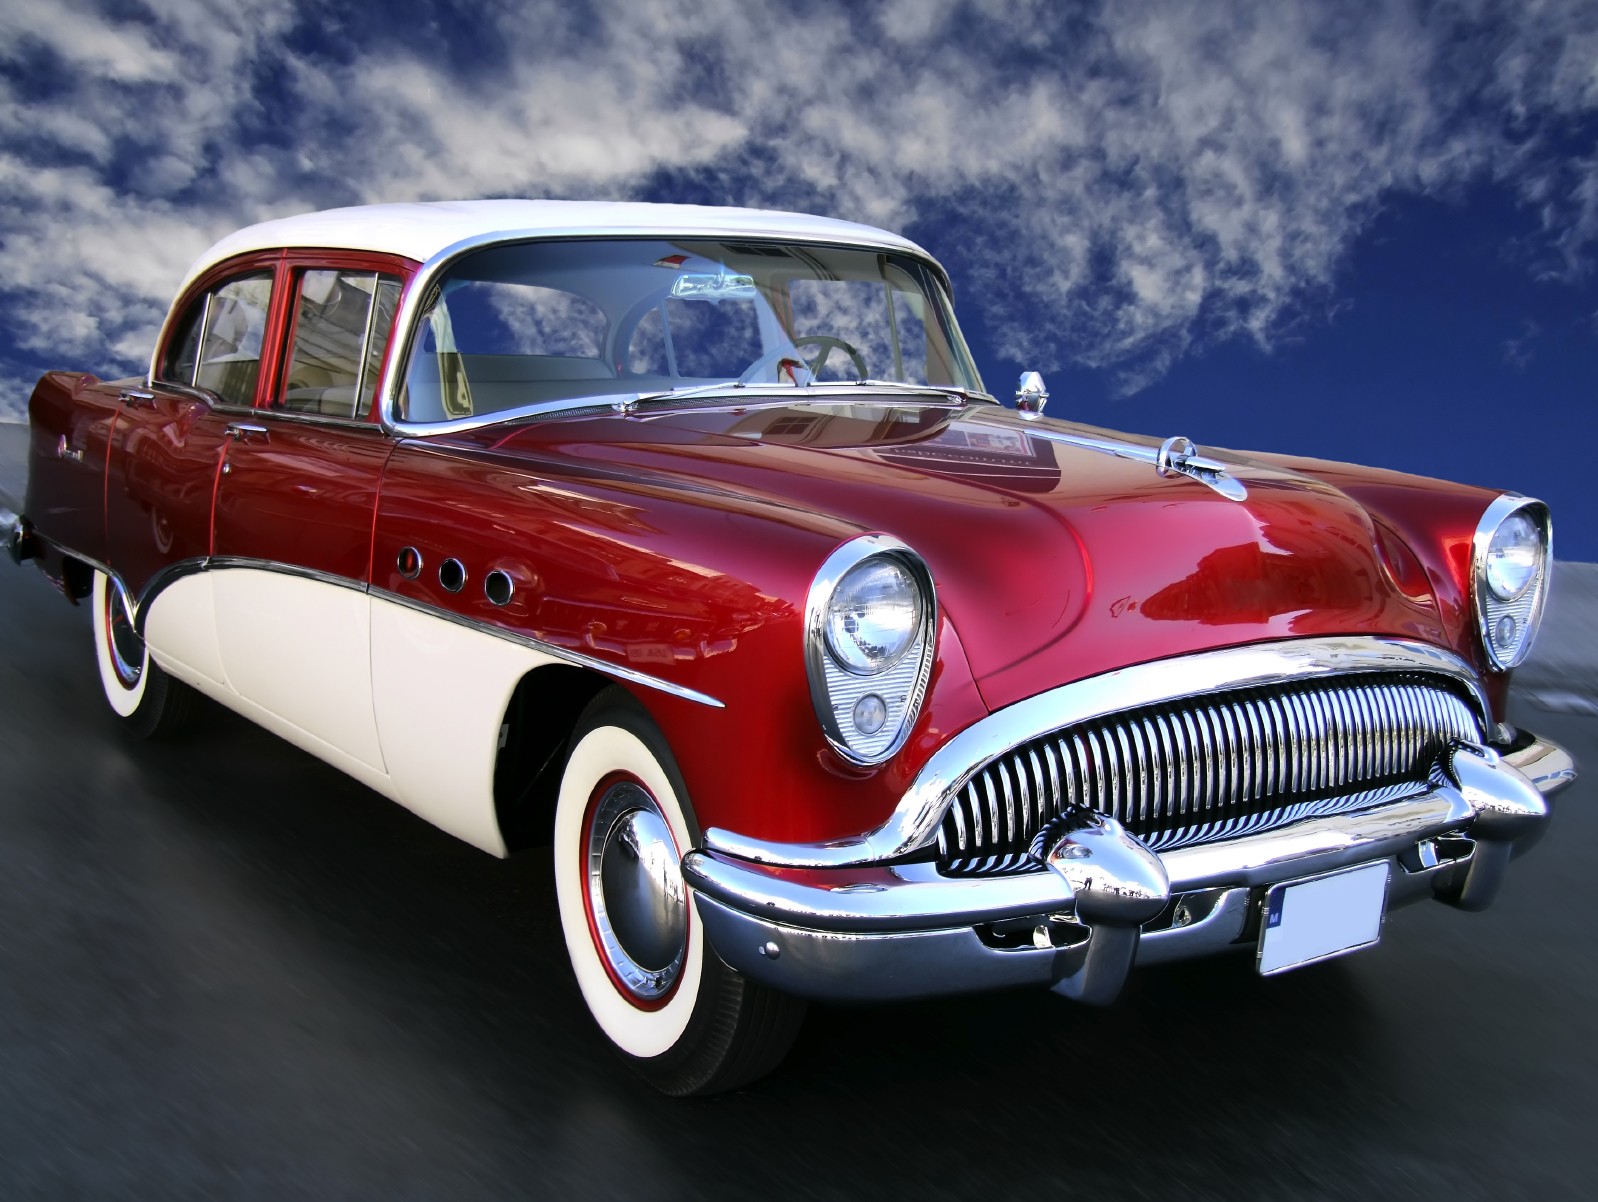
\includegraphics[width=\linewidth]{car.jpg} % content img num.3
	\end{subfigure}
	\begin{subfigure}[b]{0.225\linewidth}
		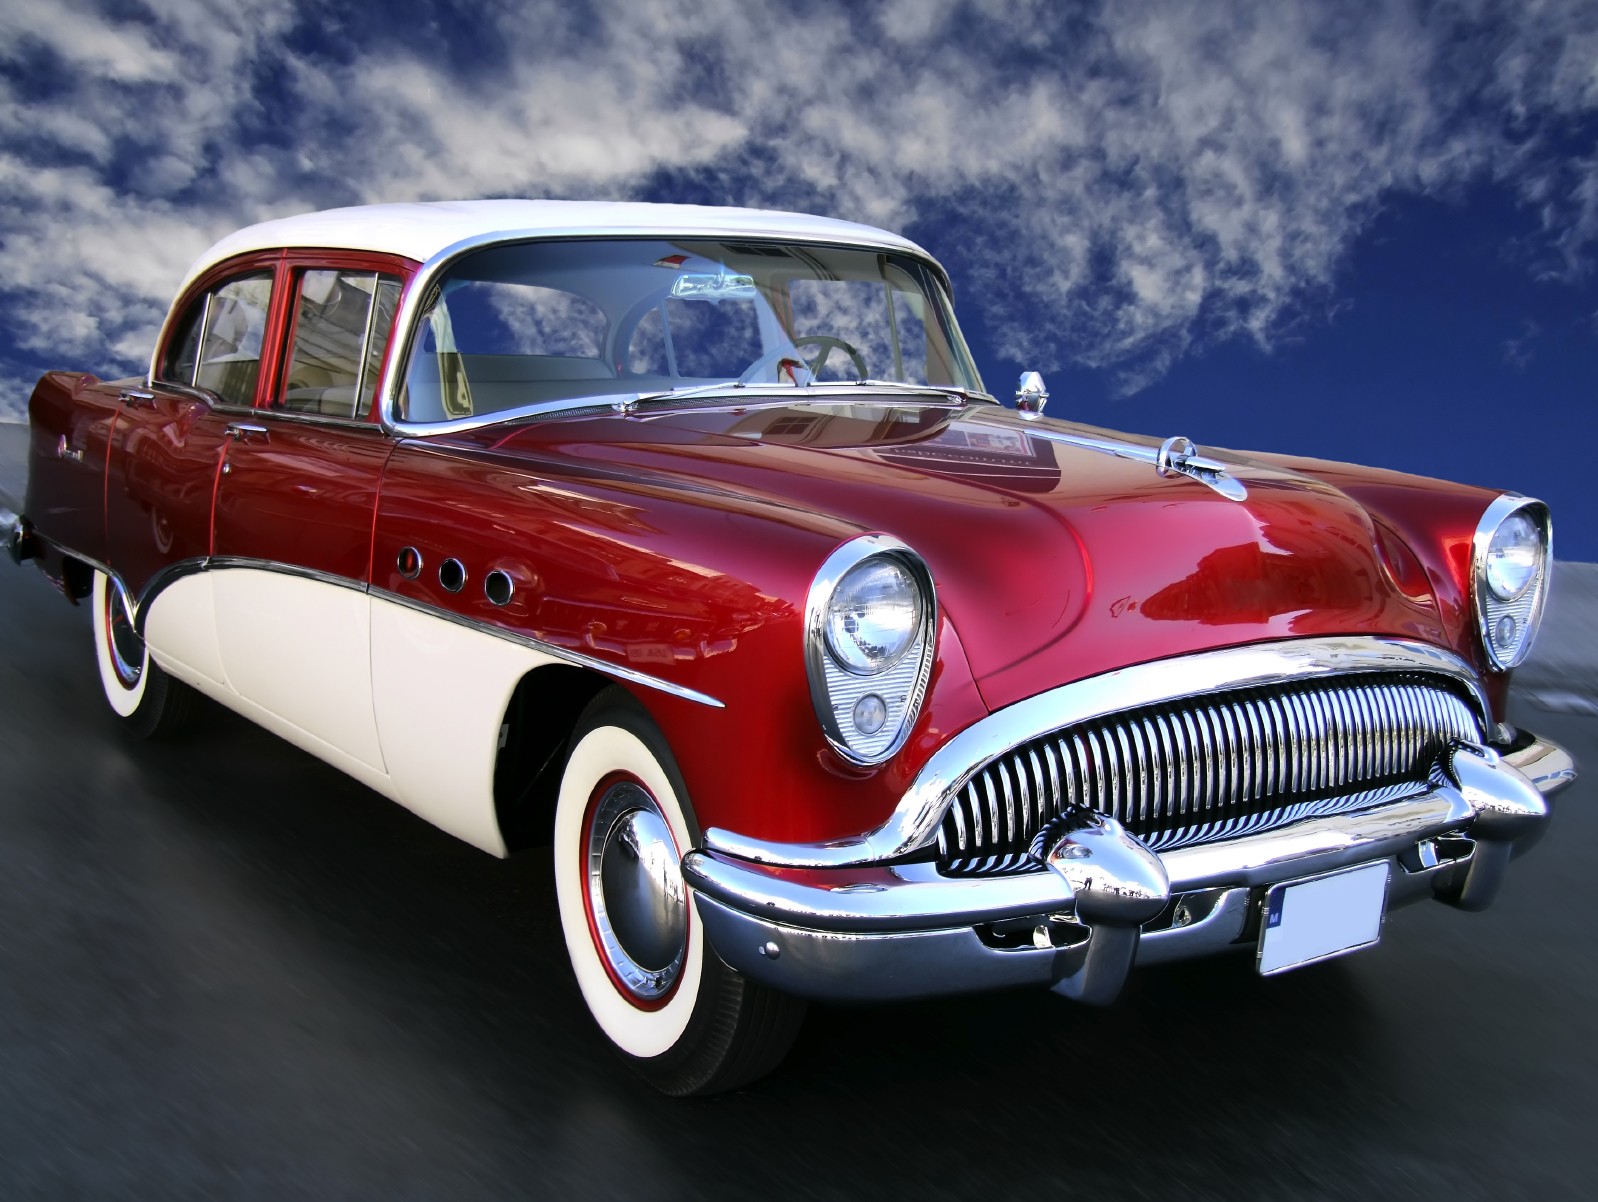
\includegraphics[width=\linewidth]{car.jpg} % theirs reconstruction num.3
	\end{subfigure}
	\begin{subfigure}[b]{0.225\linewidth}
		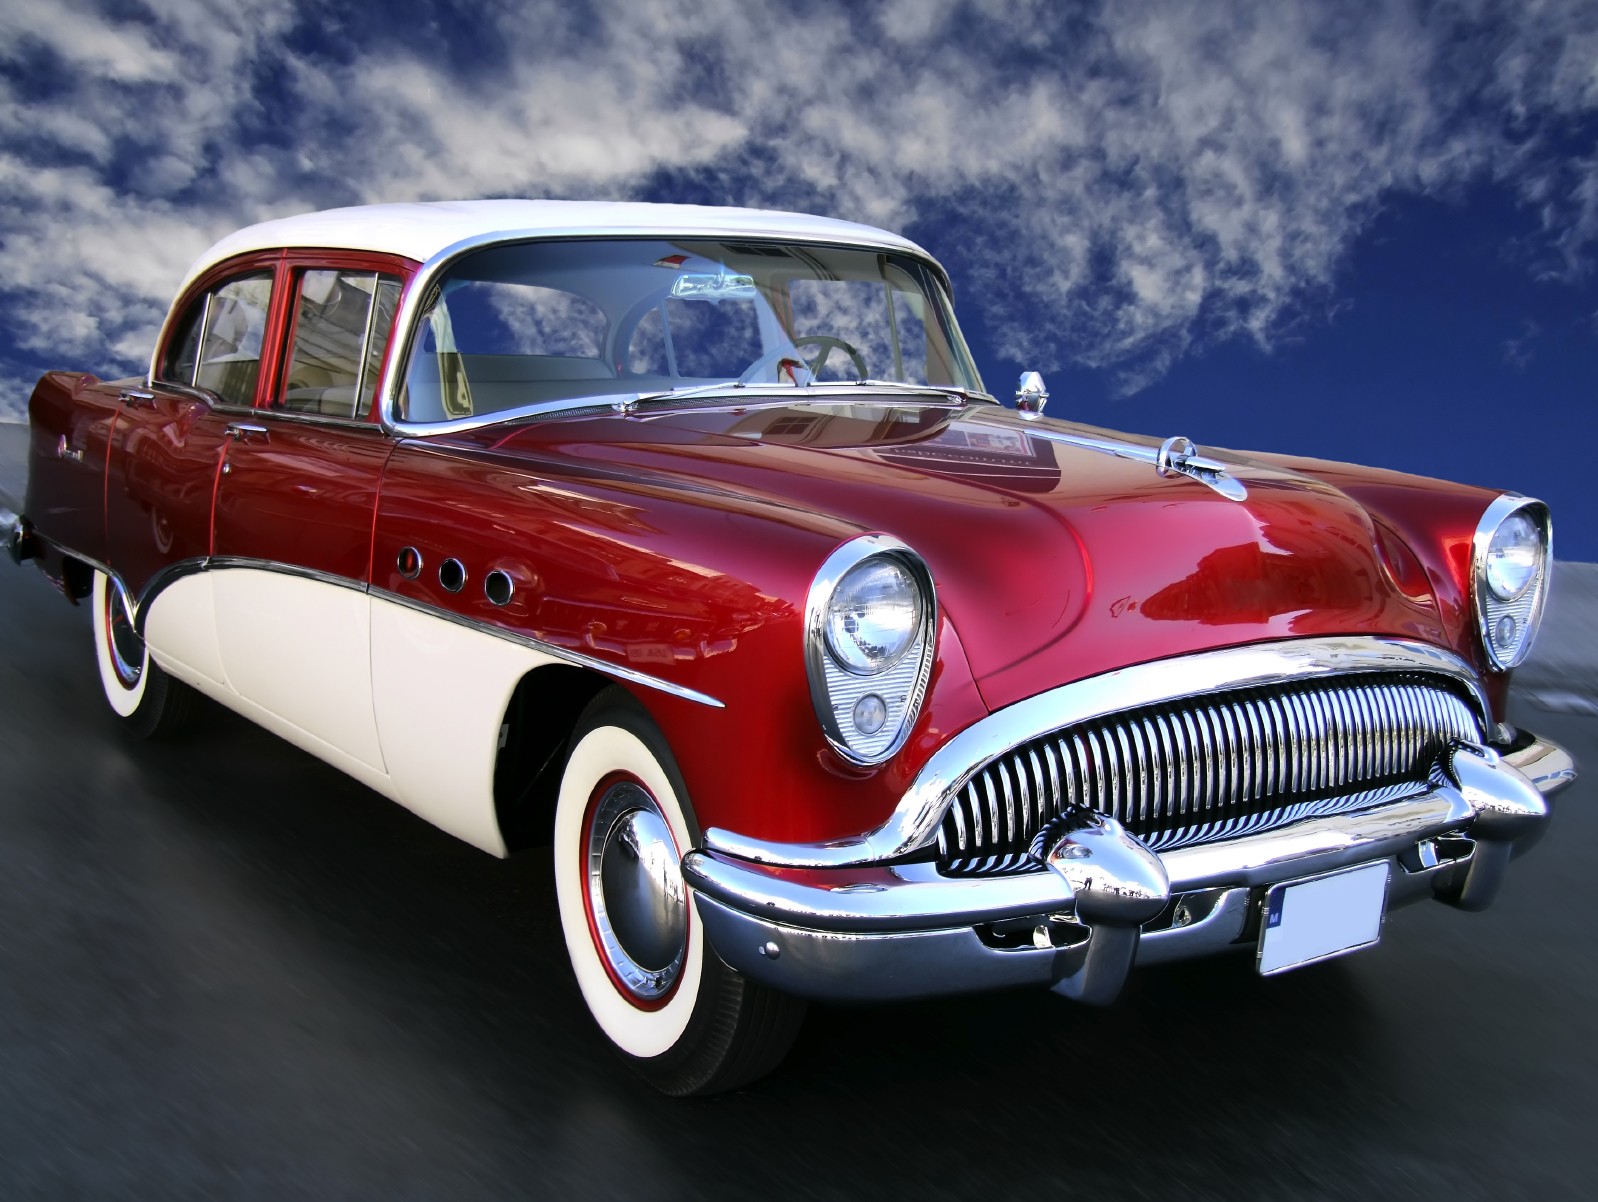
\includegraphics[width=\linewidth]{car.jpg} % ours reconstruction num.3
	\end{subfigure}
	% fourth line
	\centering
	\begin{subfigure}[b]{0.225\linewidth}
		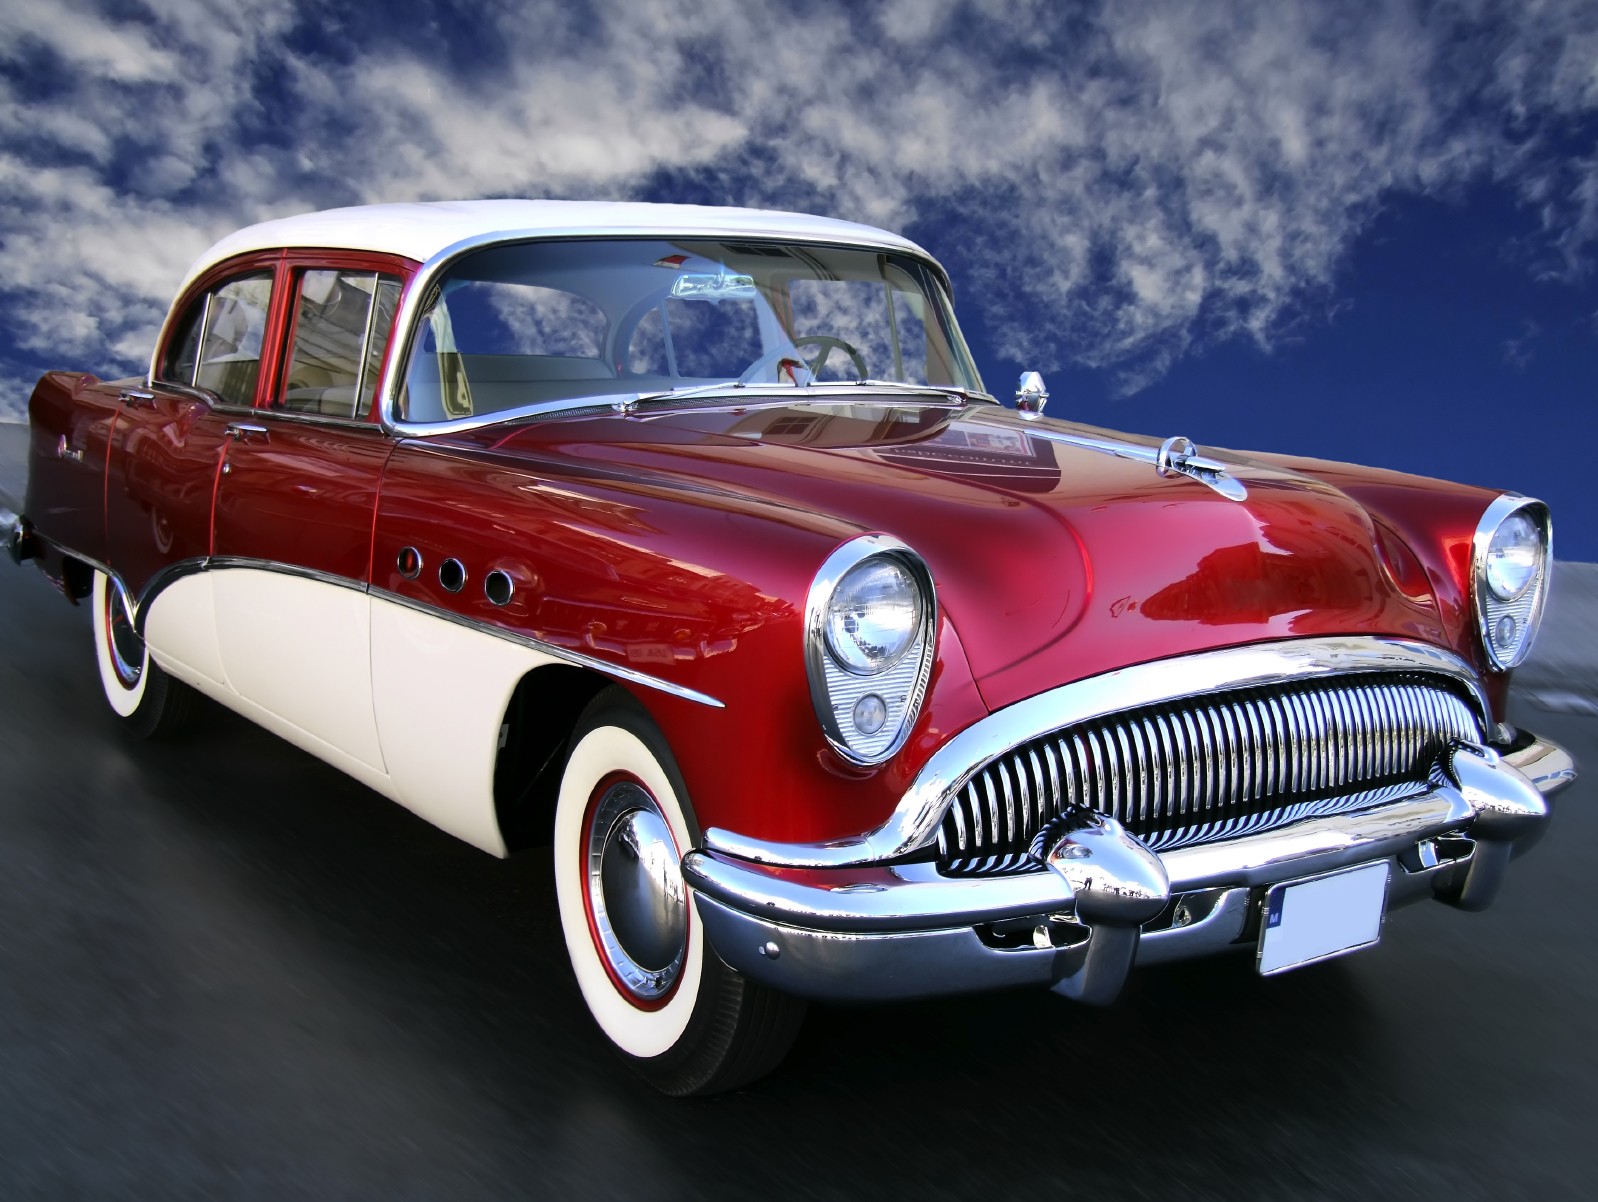
\includegraphics[width=\linewidth]{car.jpg} %style img num.4
	\end{subfigure}
	\begin{subfigure}[b]{0.225\linewidth}
		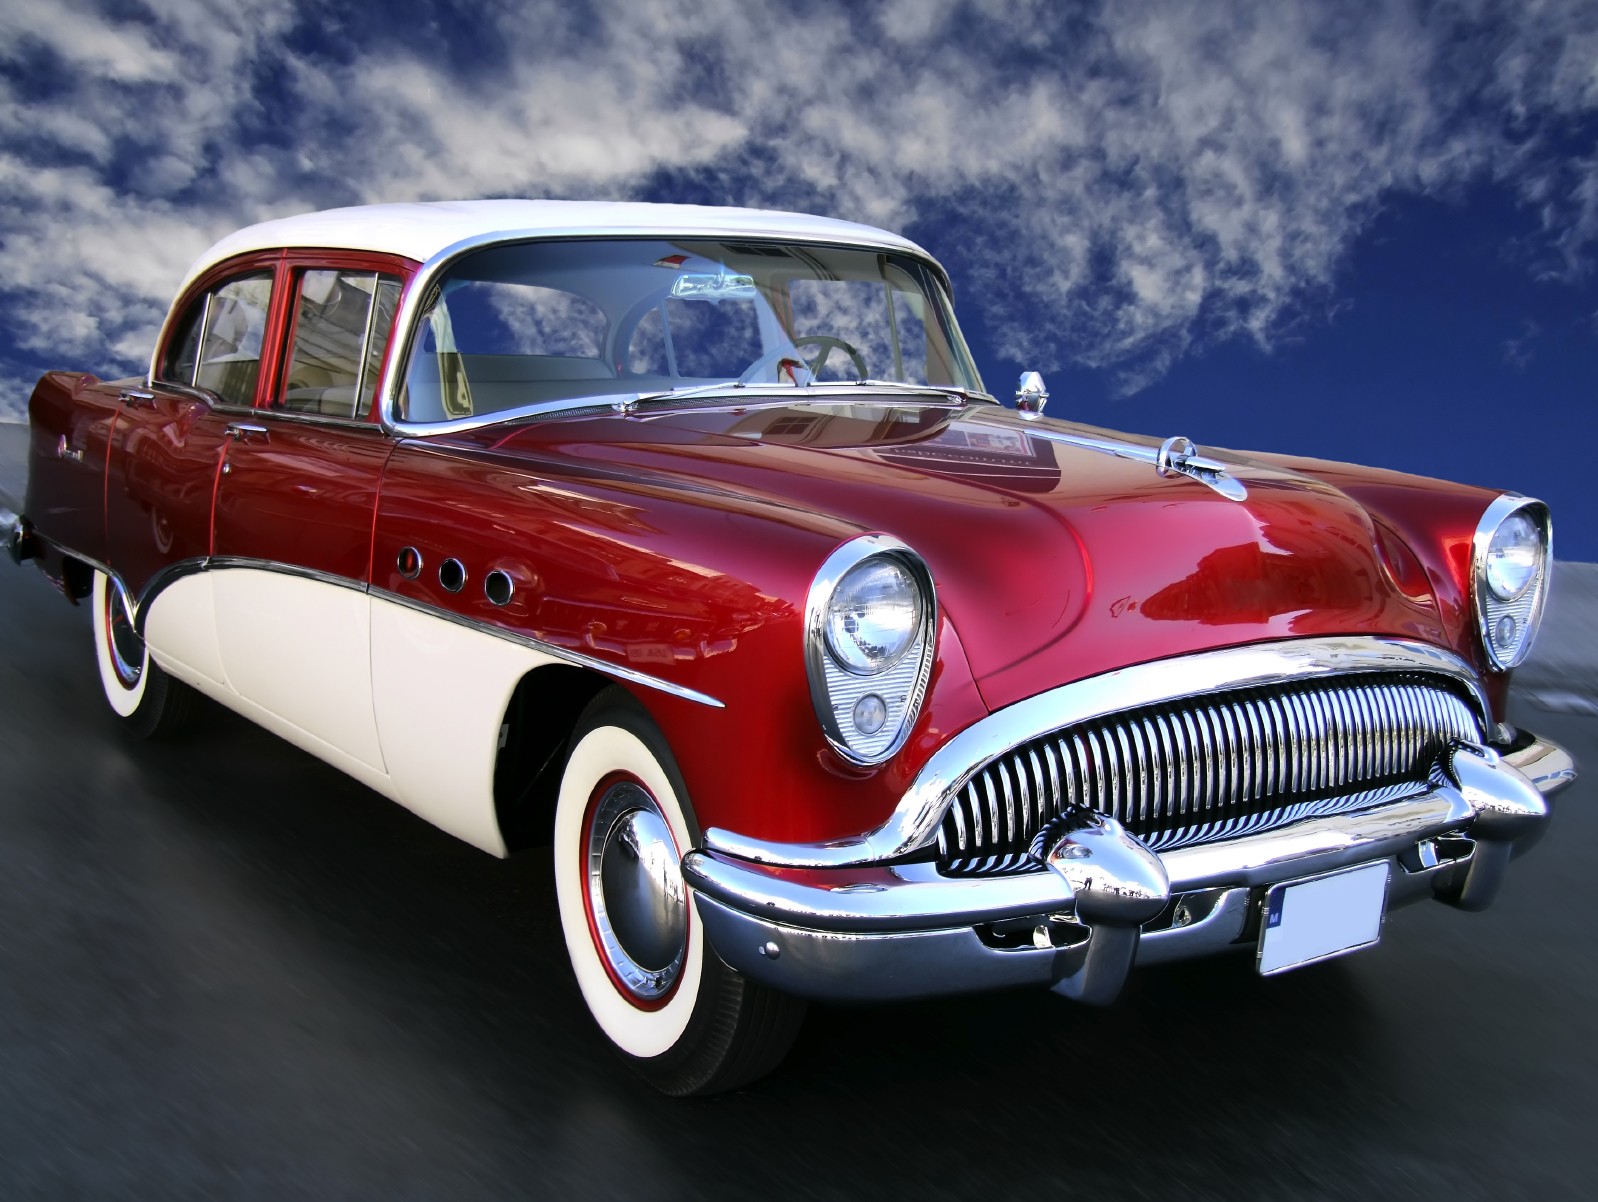
\includegraphics[width=\linewidth]{car.jpg} % content img num.4
	\end{subfigure}
	\begin{subfigure}[b]{0.225\linewidth}
		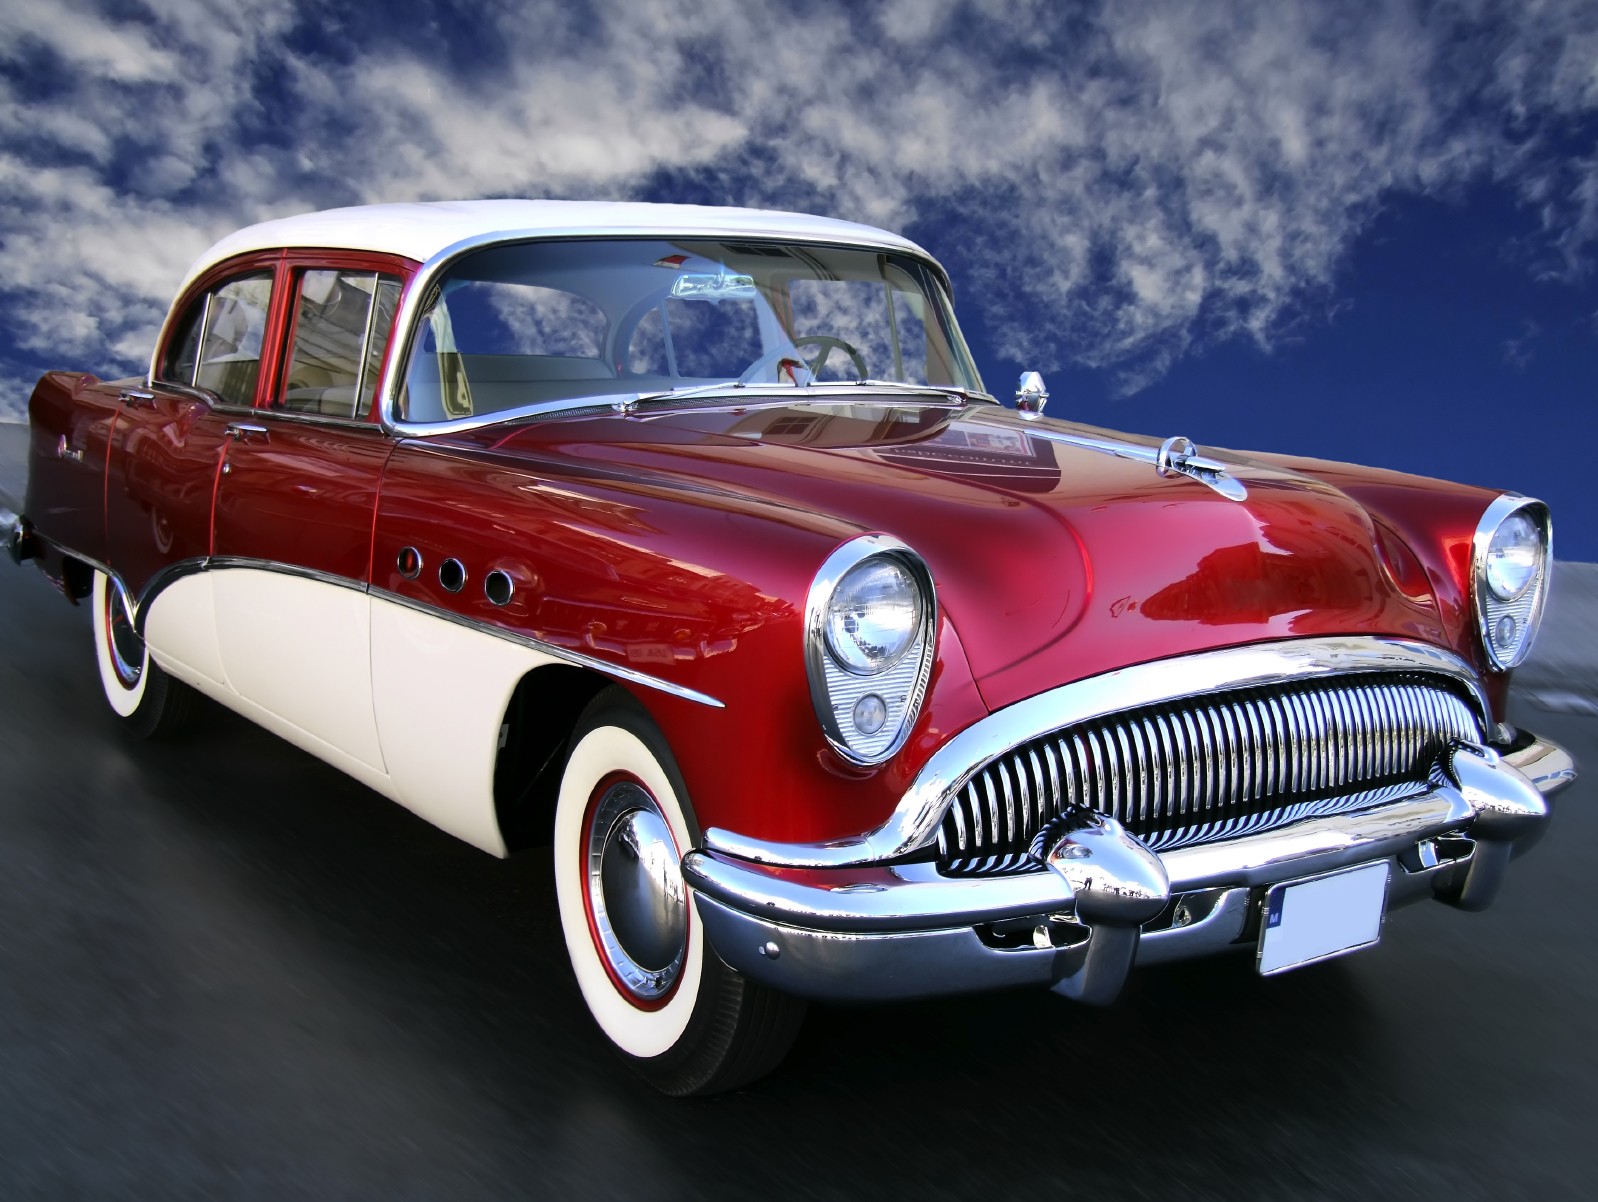
\includegraphics[width=\linewidth]{car.jpg} % theirs reconstruction num.4
	\end{subfigure}
	\begin{subfigure}[b]{0.225\linewidth}
		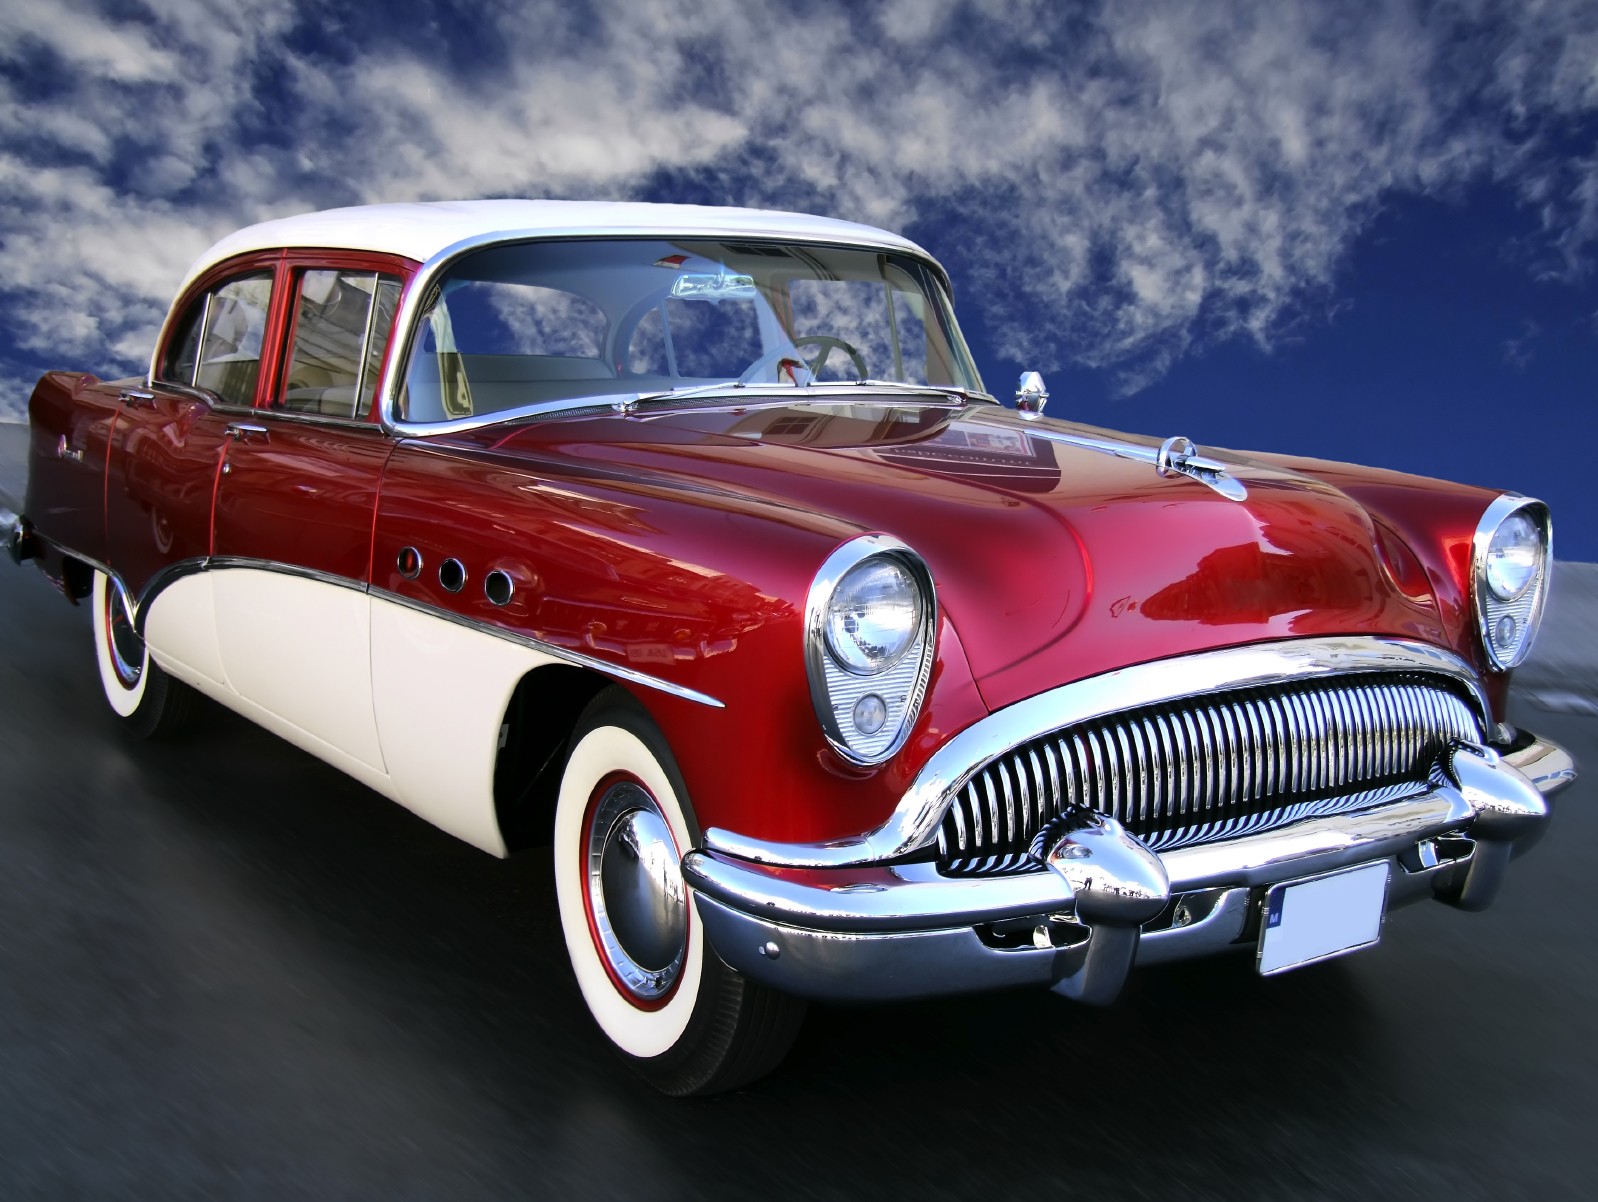
\includegraphics[width=\linewidth]{car.jpg} % ours reconstruction num.4
	\end{subfigure}
	% fifth line
	\centering
	\begin{subfigure}[b]{0.225\linewidth}
		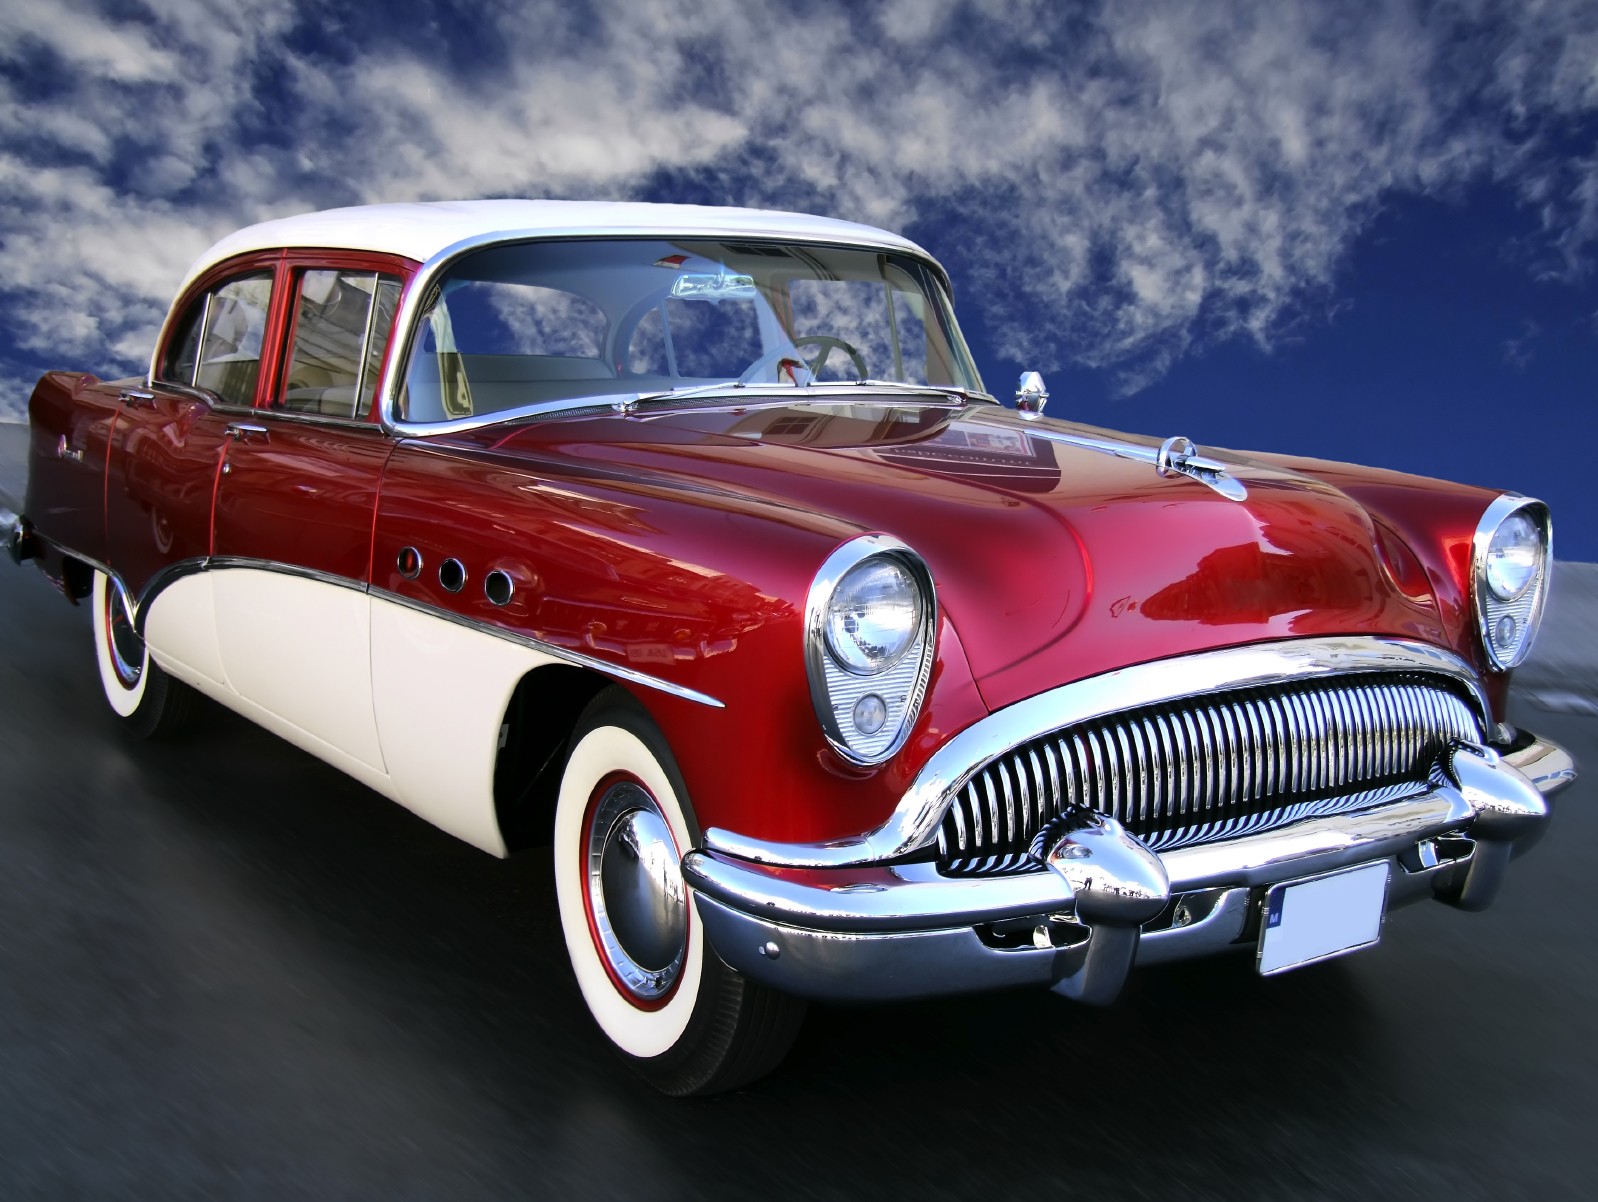
\includegraphics[width=\linewidth]{car.jpg} %style img num.5
		\caption{Style}
	\end{subfigure}
	\begin{subfigure}[b]{0.225\linewidth}
		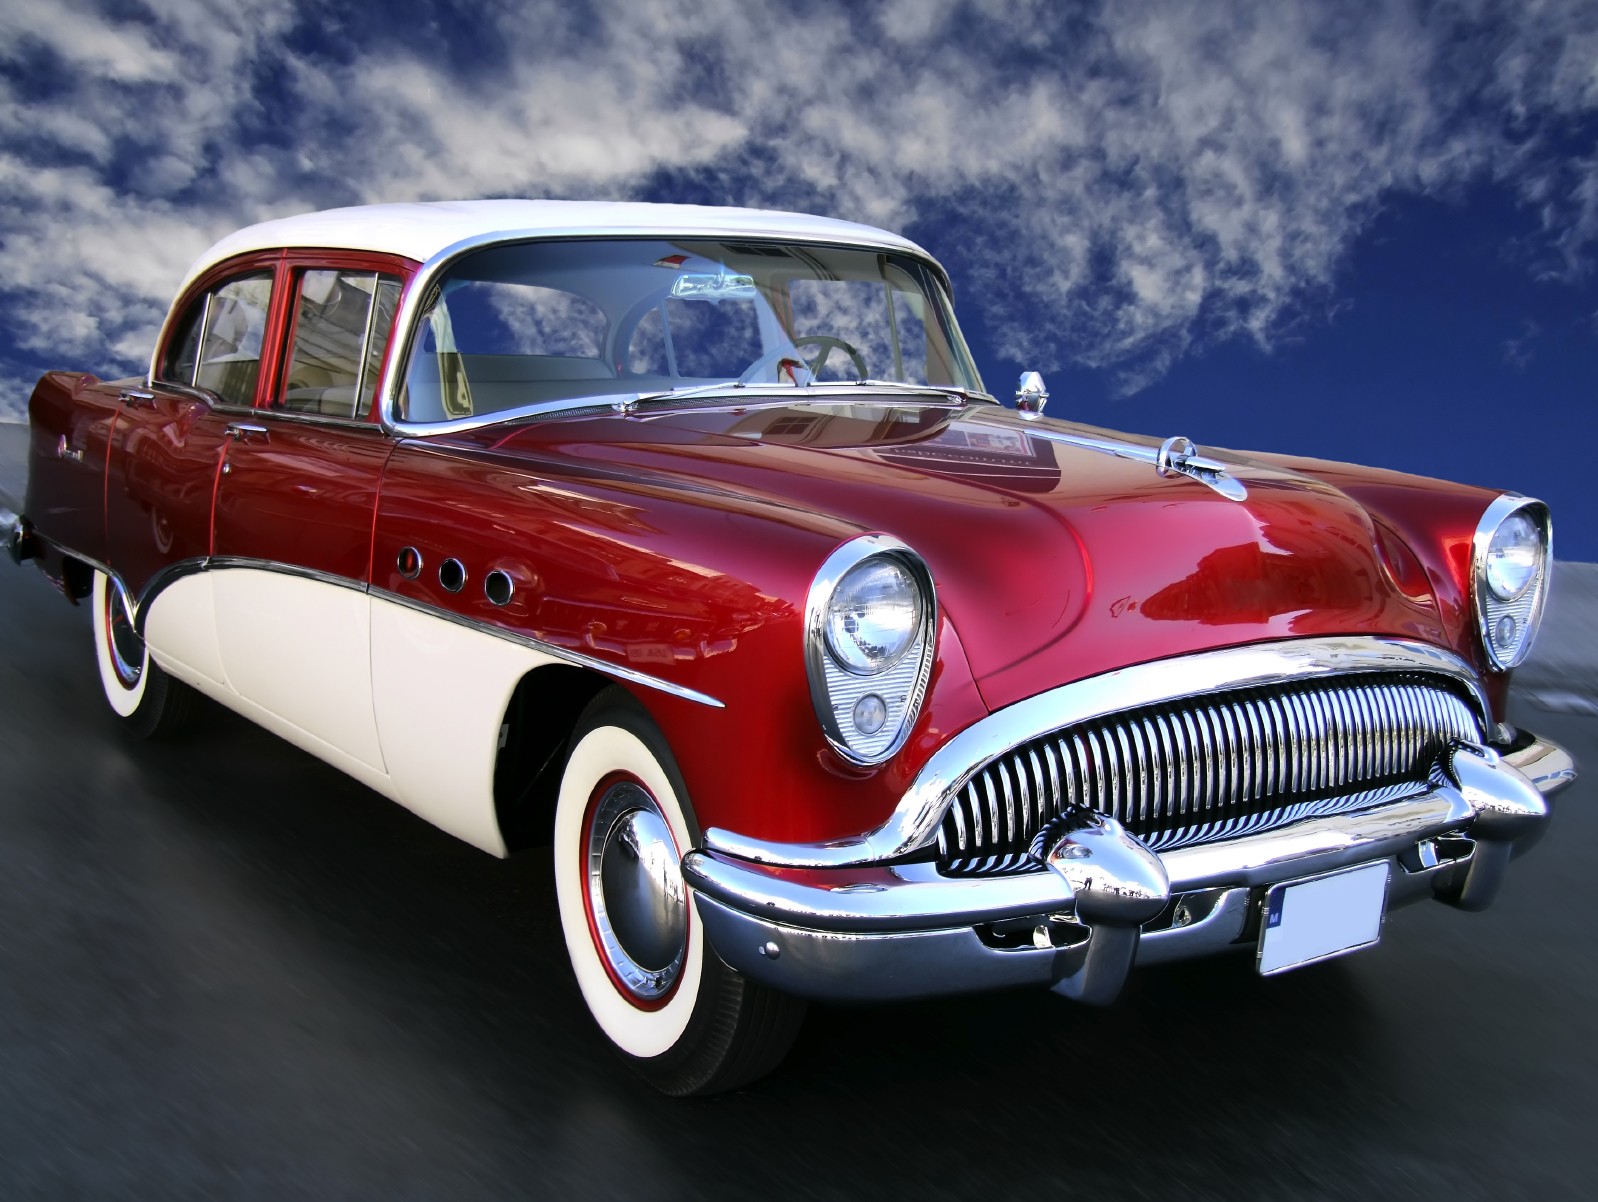
\includegraphics[width=\linewidth]{car.jpg} % content img num.5
		\caption{Content}
	\end{subfigure}
	\begin{subfigure}[b]{0.225\linewidth}
		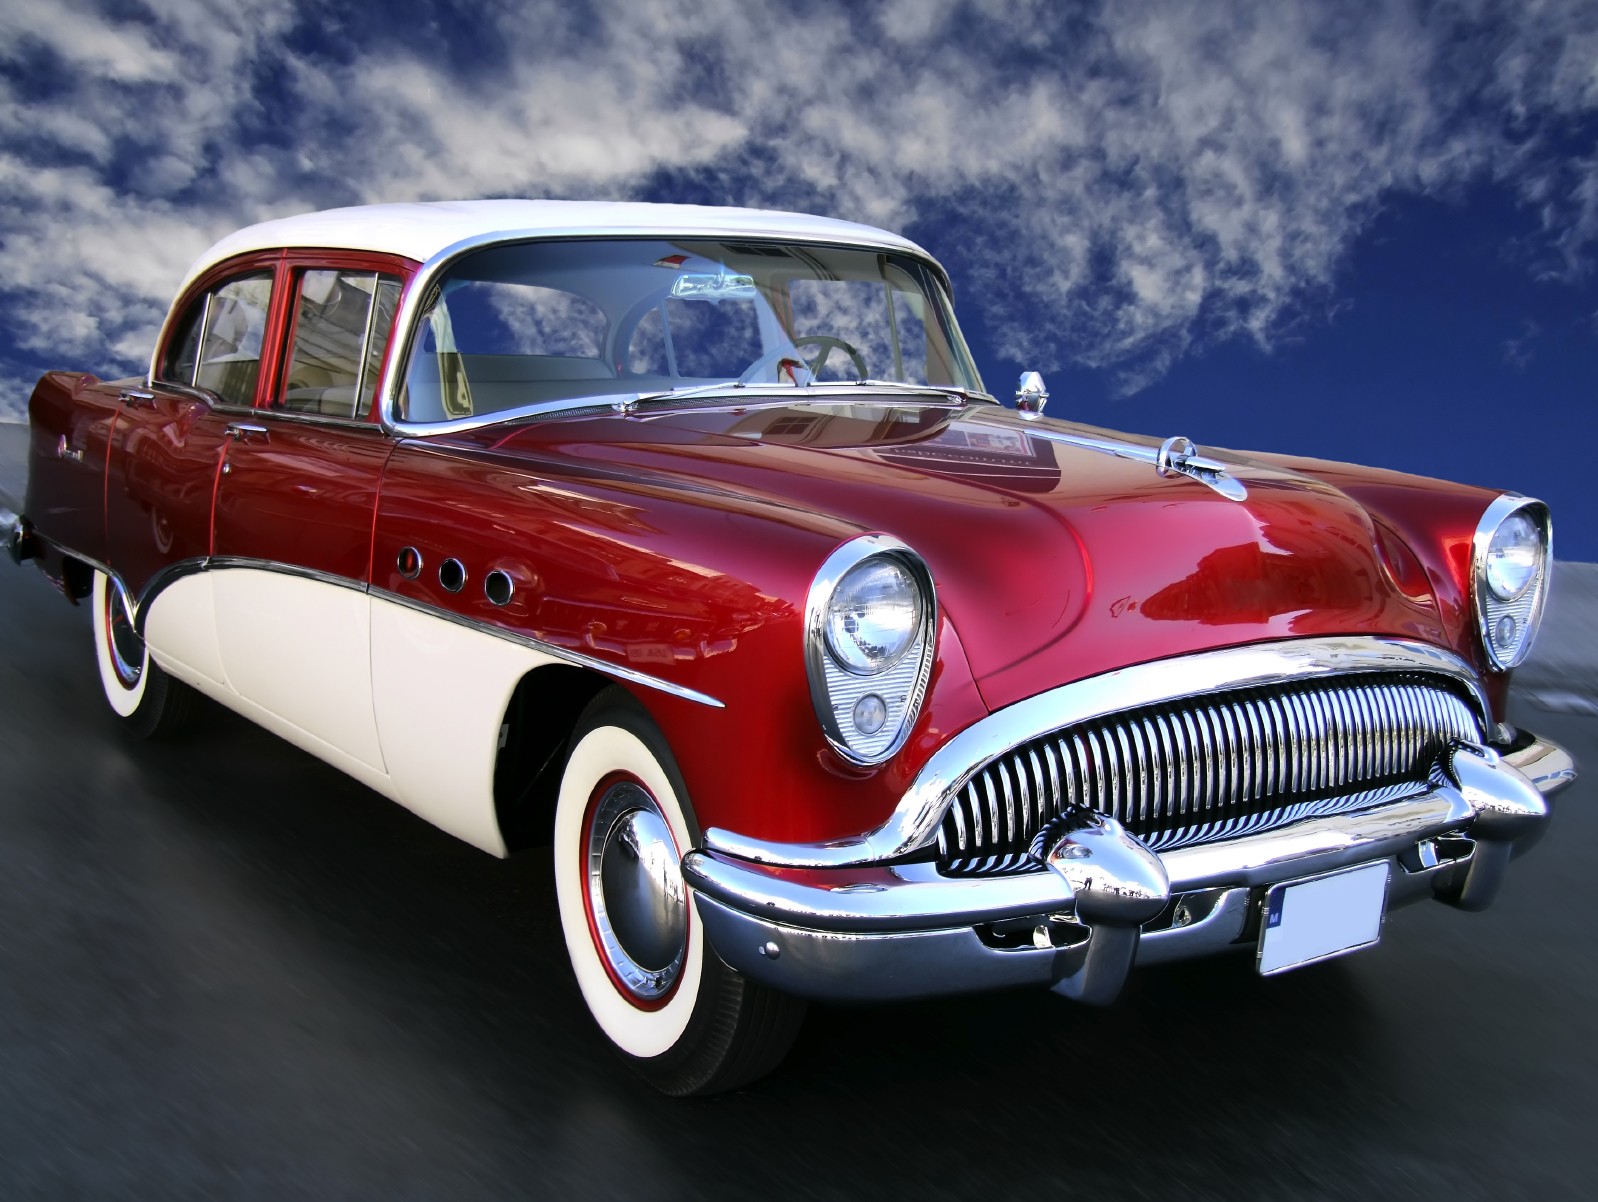
\includegraphics[width=\linewidth]{car.jpg} % theirs reconstruction num.5
		\caption{Li et al. \cite{bib11}}
	\end{subfigure}
	\begin{subfigure}[b]{0.225\linewidth}
		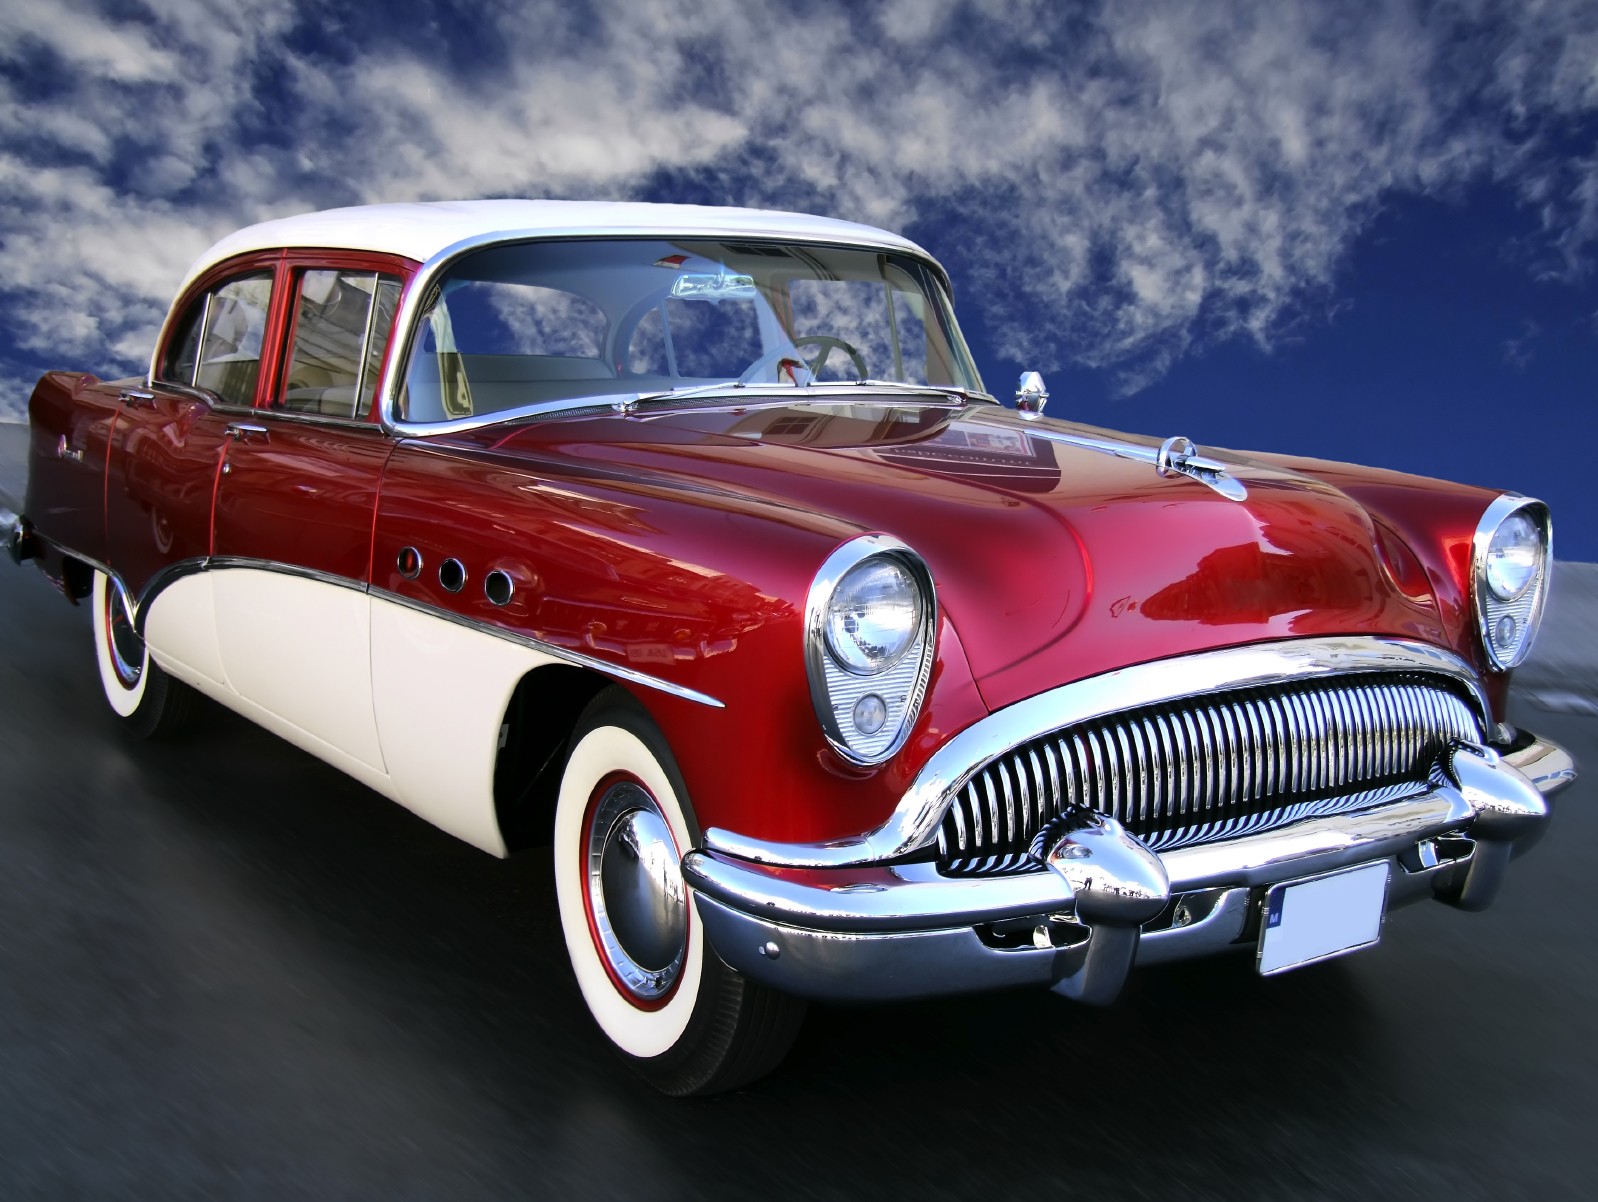
\includegraphics[width=\linewidth]{car.jpg} % ours reconstruction num.5
		\caption{Our implementation}
	\end{subfigure}
	\caption{Results from different style transfer methods using style weight $\alpha=0.5$}
	\label{fig:style_transfer}
\end{figure}
%%%%%%%%%%%%%%%%%%%%%%%%%%%%
%%%%%%%%%%%%%%%%%%%%%%%%%%%%
% Boost %
%%%%%%%%%%%%%%%%%%%%%%%%%%%%
%%%%%%%%%%%%%%%%%%%%%%%%%%%%
\subsubsection{Stylization boosting}
\begin{figure}[H]
	% first line
	\centering
	\begin{subfigure}[b]{0.225\linewidth}
		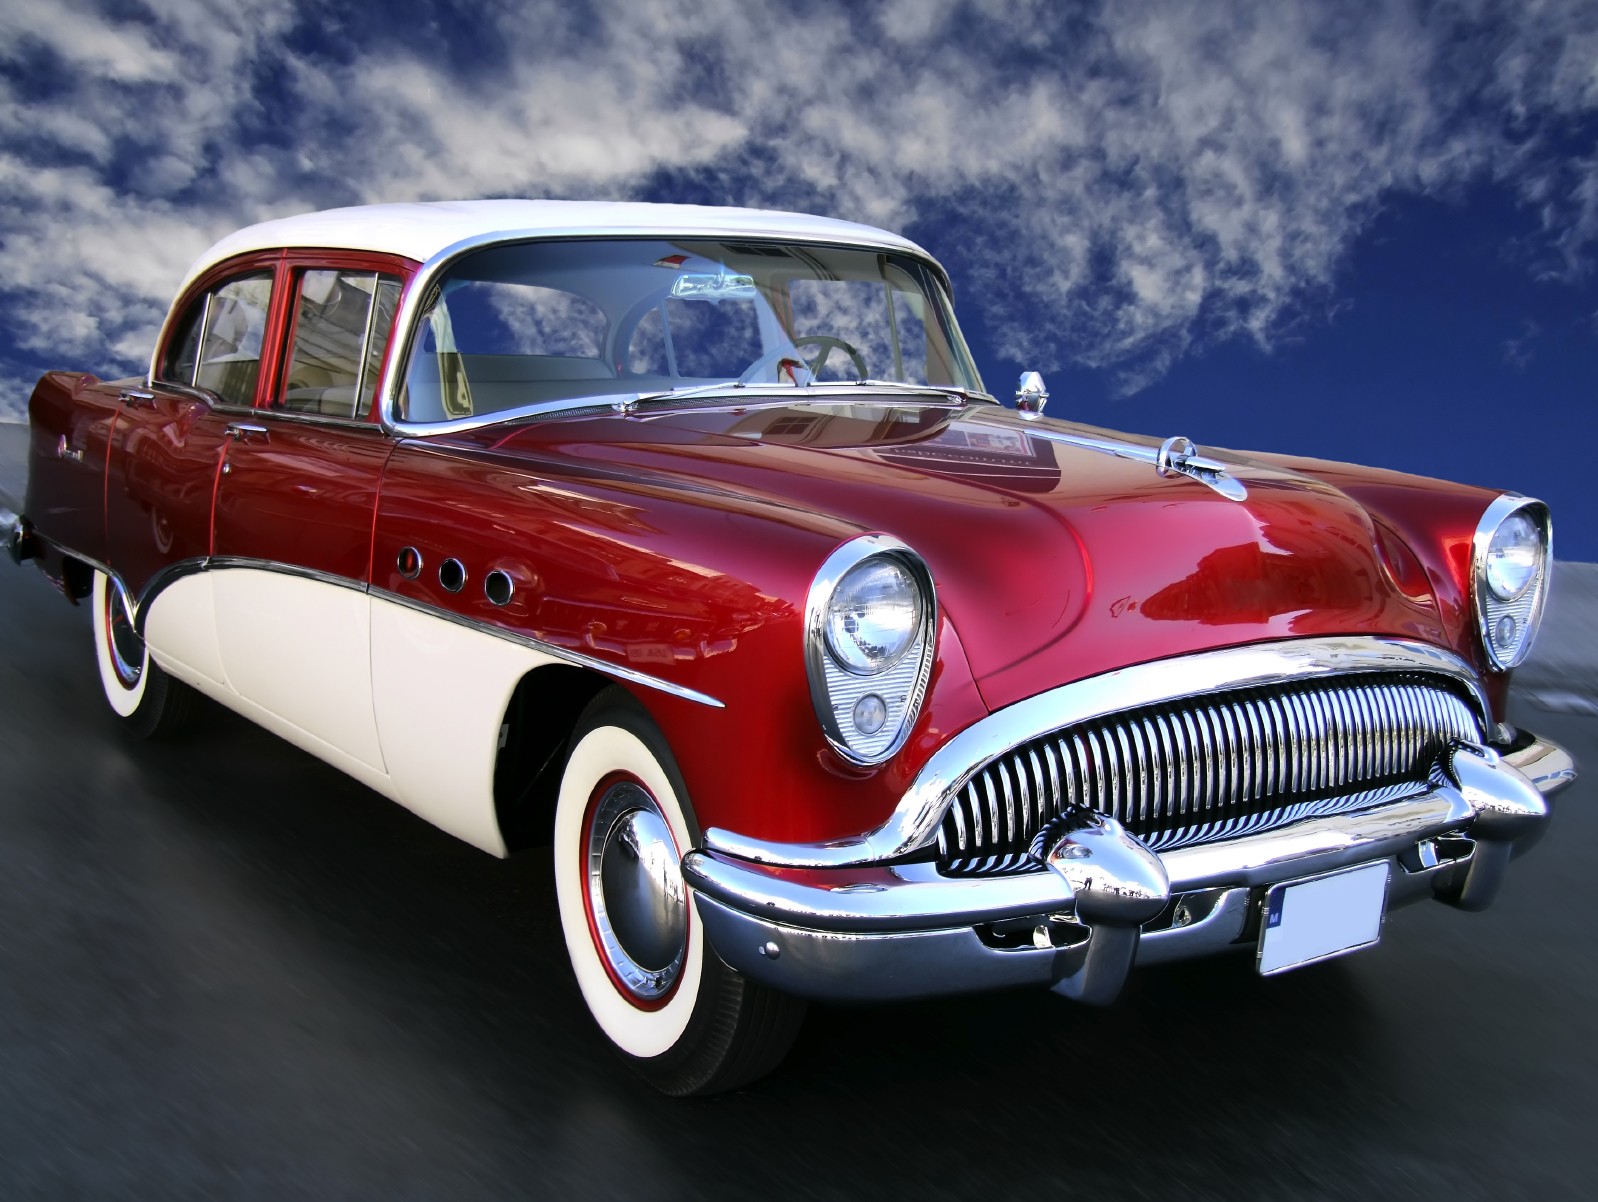
\includegraphics[width=\linewidth]{car.jpg} %style img num.1
	\end{subfigure}
	\begin{subfigure}[b]{0.225\linewidth}
		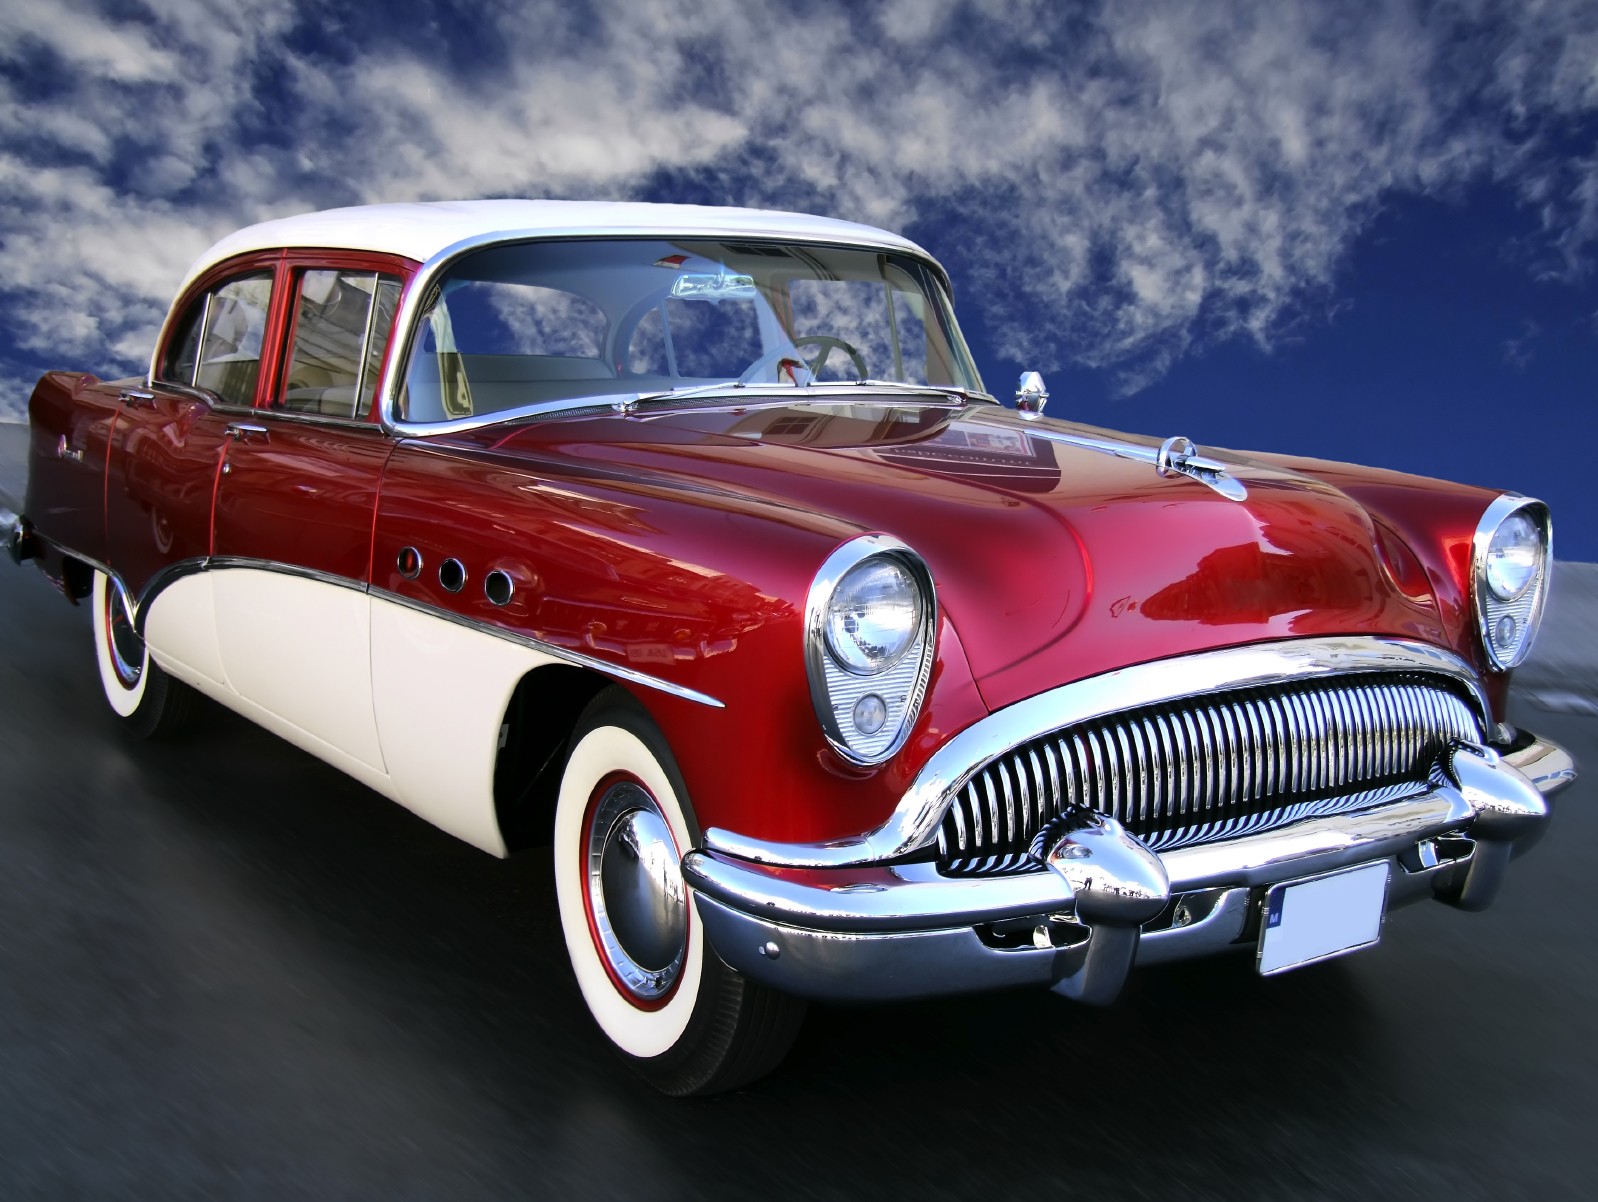
\includegraphics[width=\linewidth]{car.jpg} % content img num.1
	\end{subfigure}
	\begin{subfigure}[b]{0.225\linewidth}
		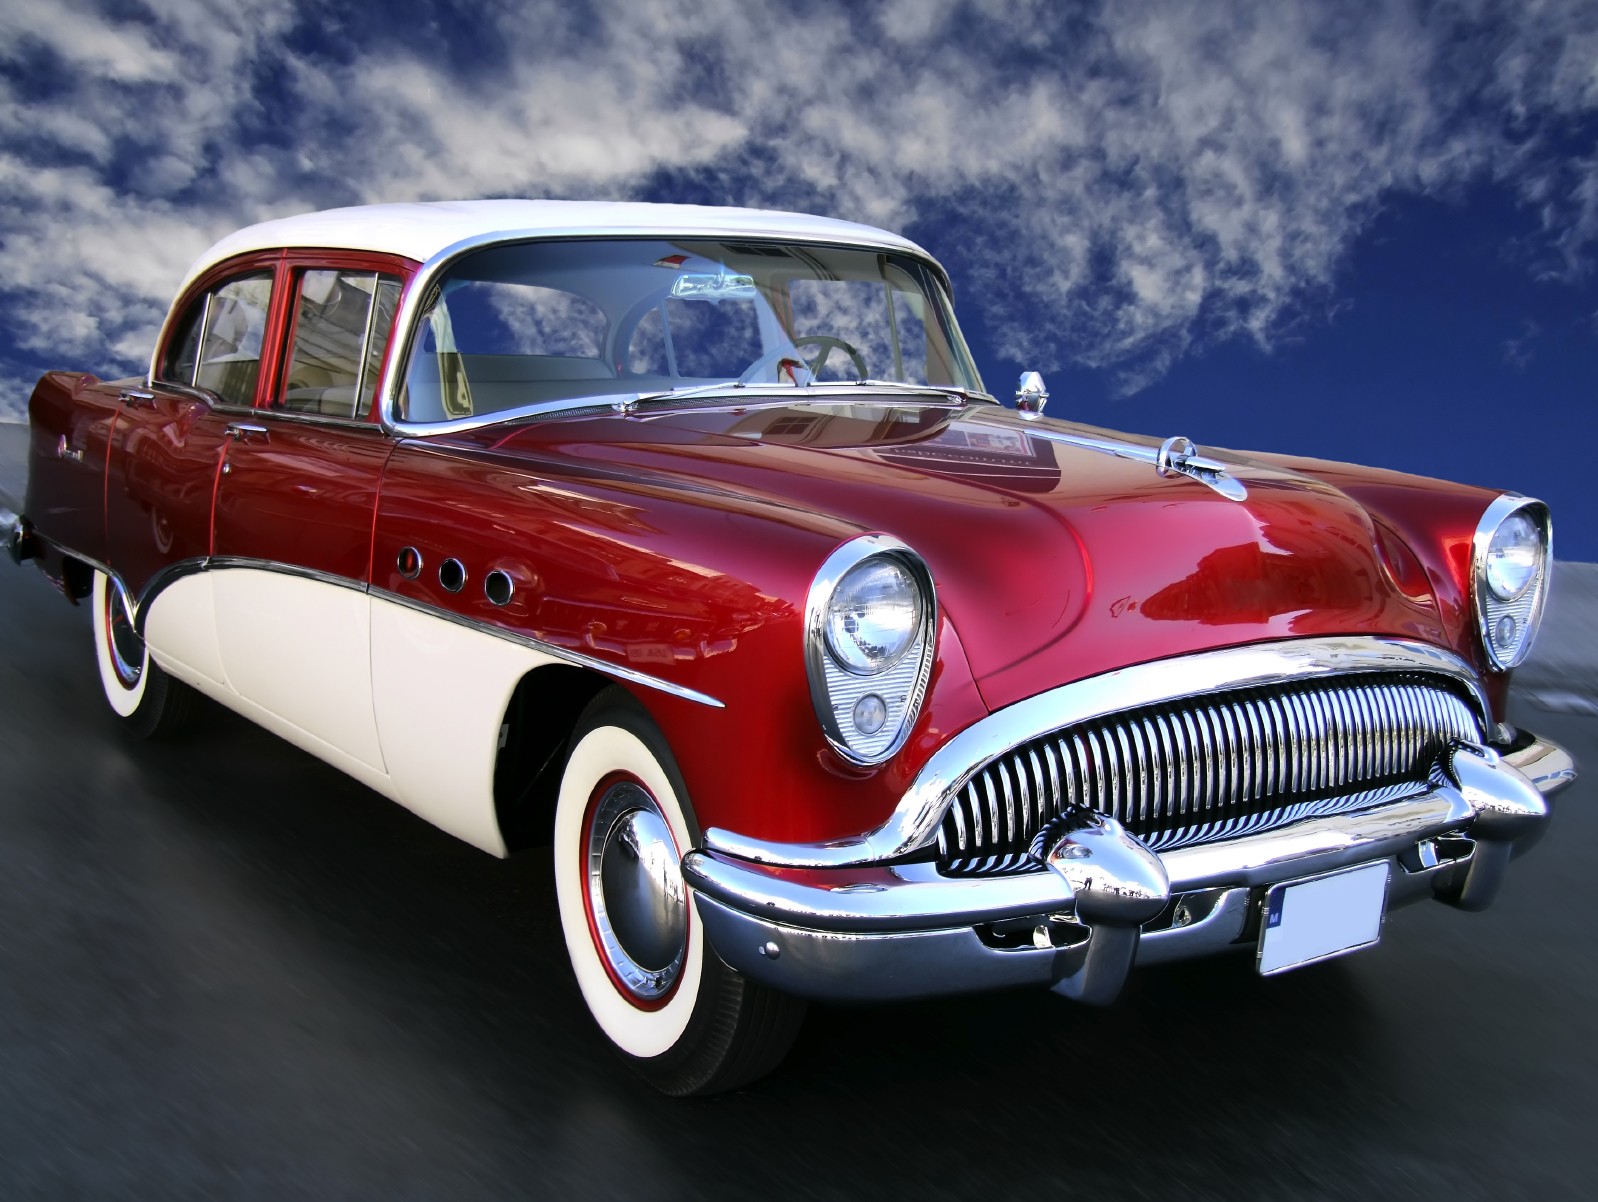
\includegraphics[width=\linewidth]{car.jpg} % regular UST num.1
	\end{subfigure}
	\begin{subfigure}[b]{0.225\linewidth}
		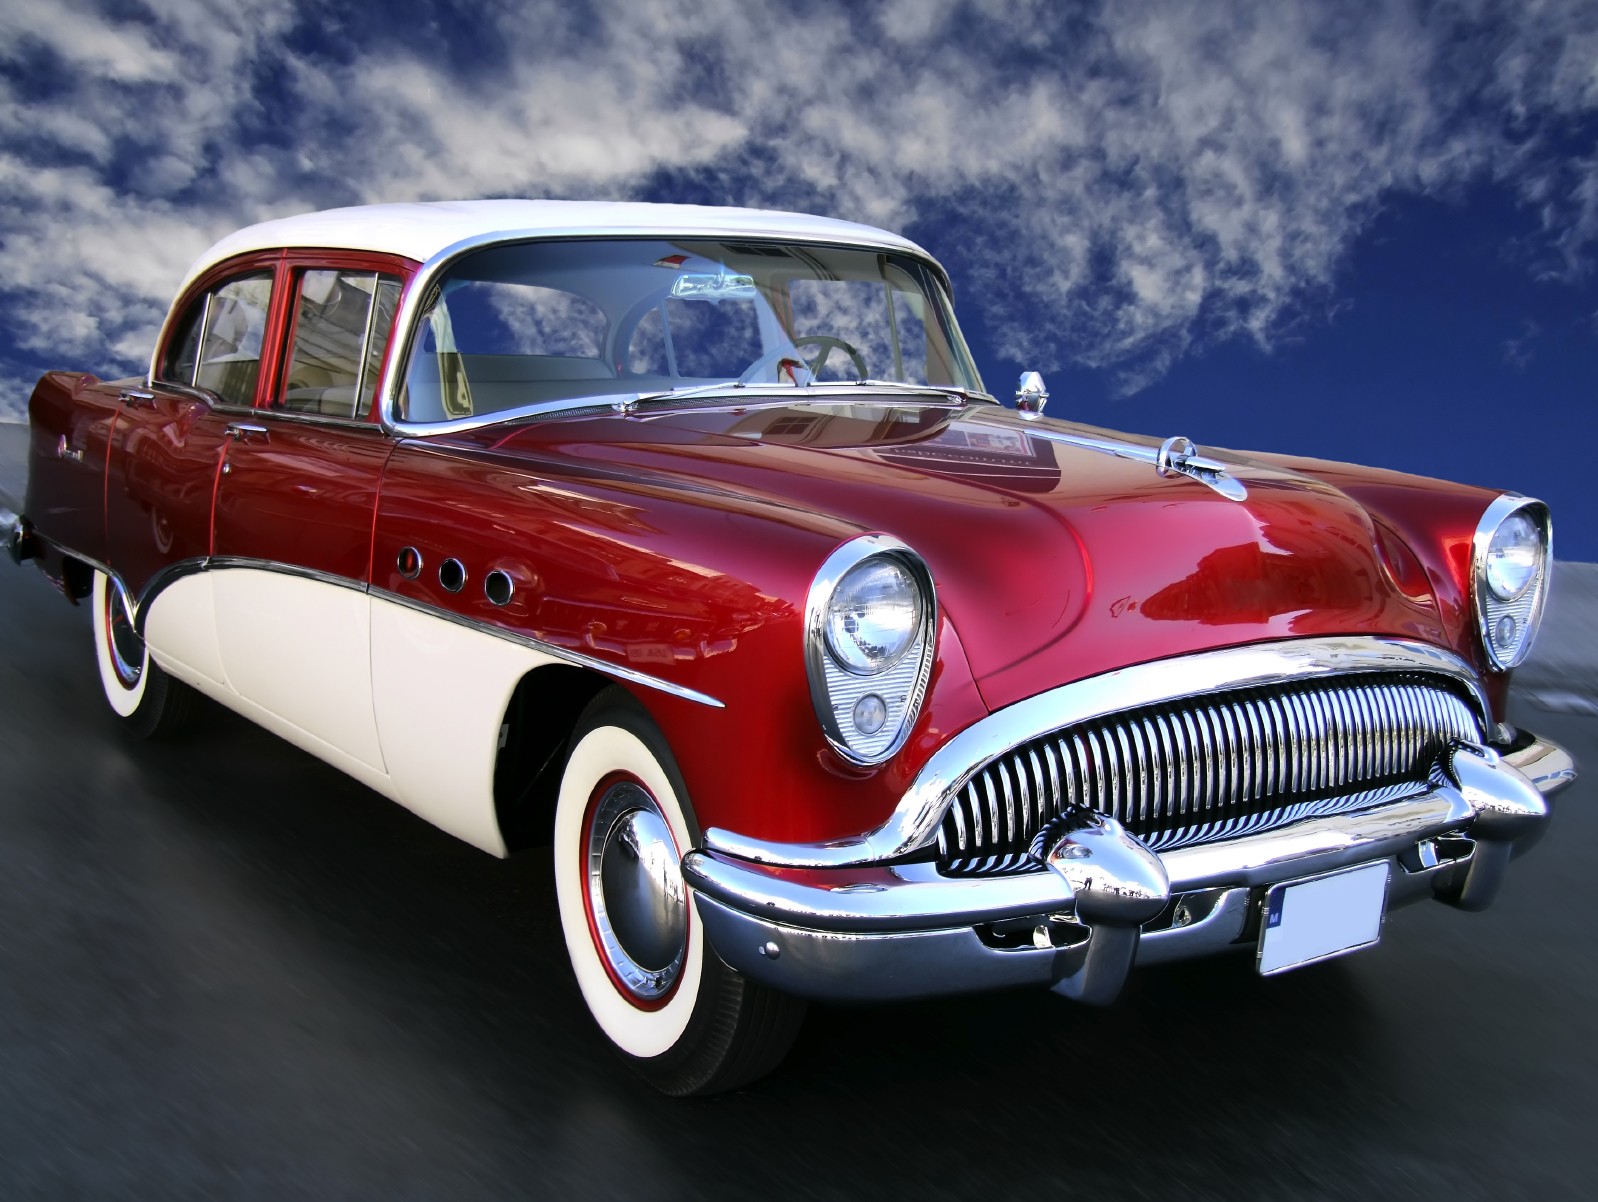
\includegraphics[width=\linewidth]{car.jpg} % UST+boost num.1
	\end{subfigure}
	% second line
	\centering
	\begin{subfigure}[b]{0.225\linewidth}
		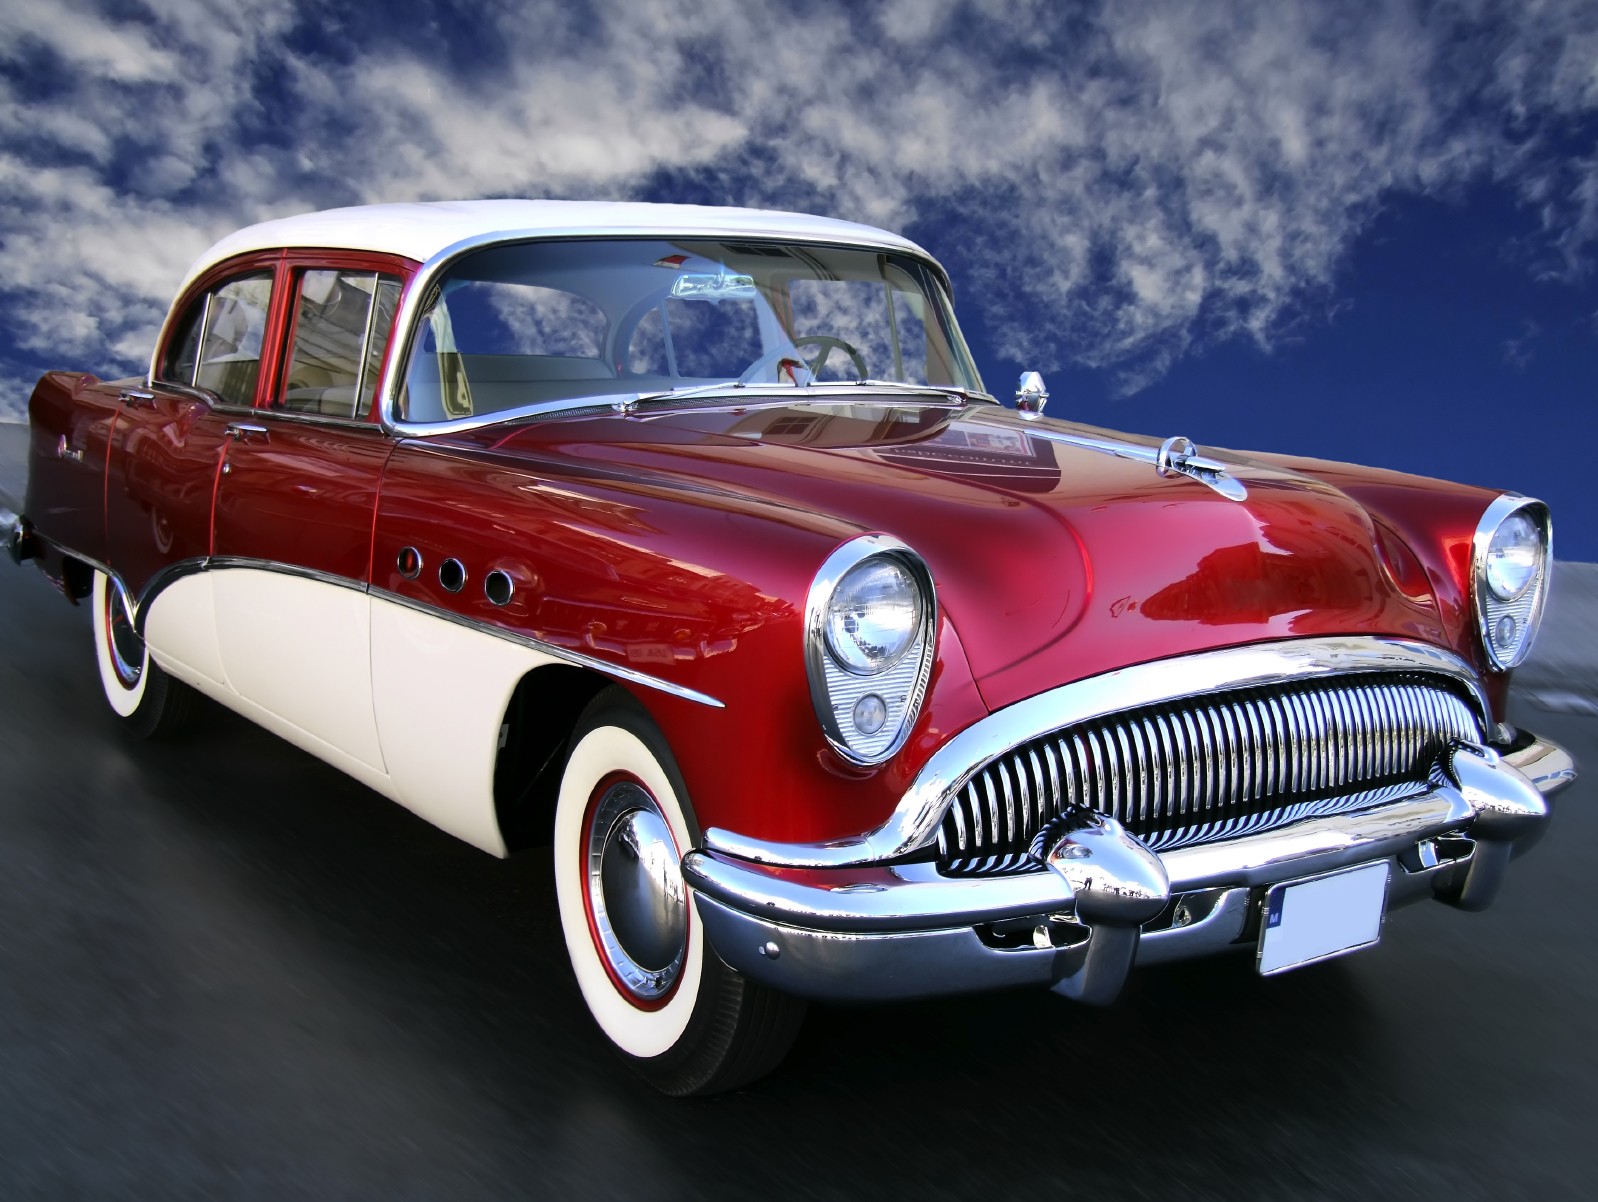
\includegraphics[width=\linewidth]{car.jpg} %style img num.2
	\end{subfigure}
	\begin{subfigure}[b]{0.225\linewidth}
		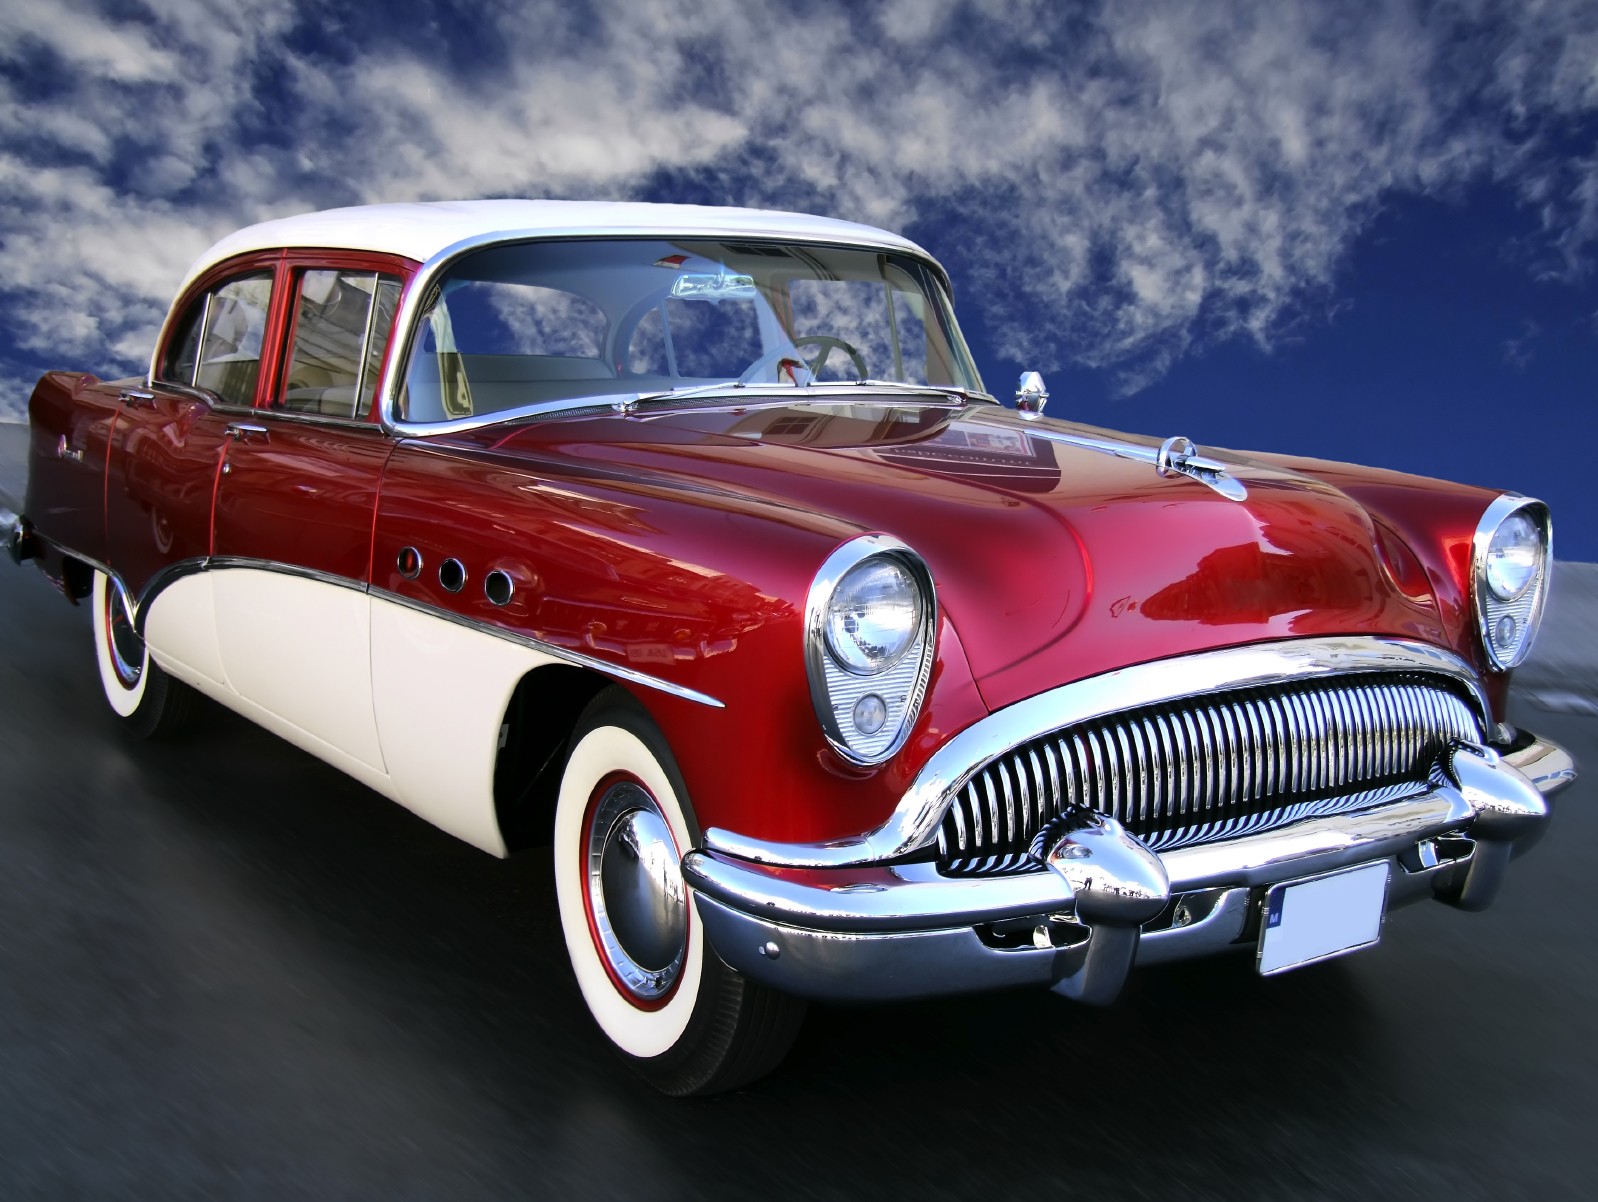
\includegraphics[width=\linewidth]{car.jpg} % content img num.2
	\end{subfigure}
	\begin{subfigure}[b]{0.225\linewidth}
		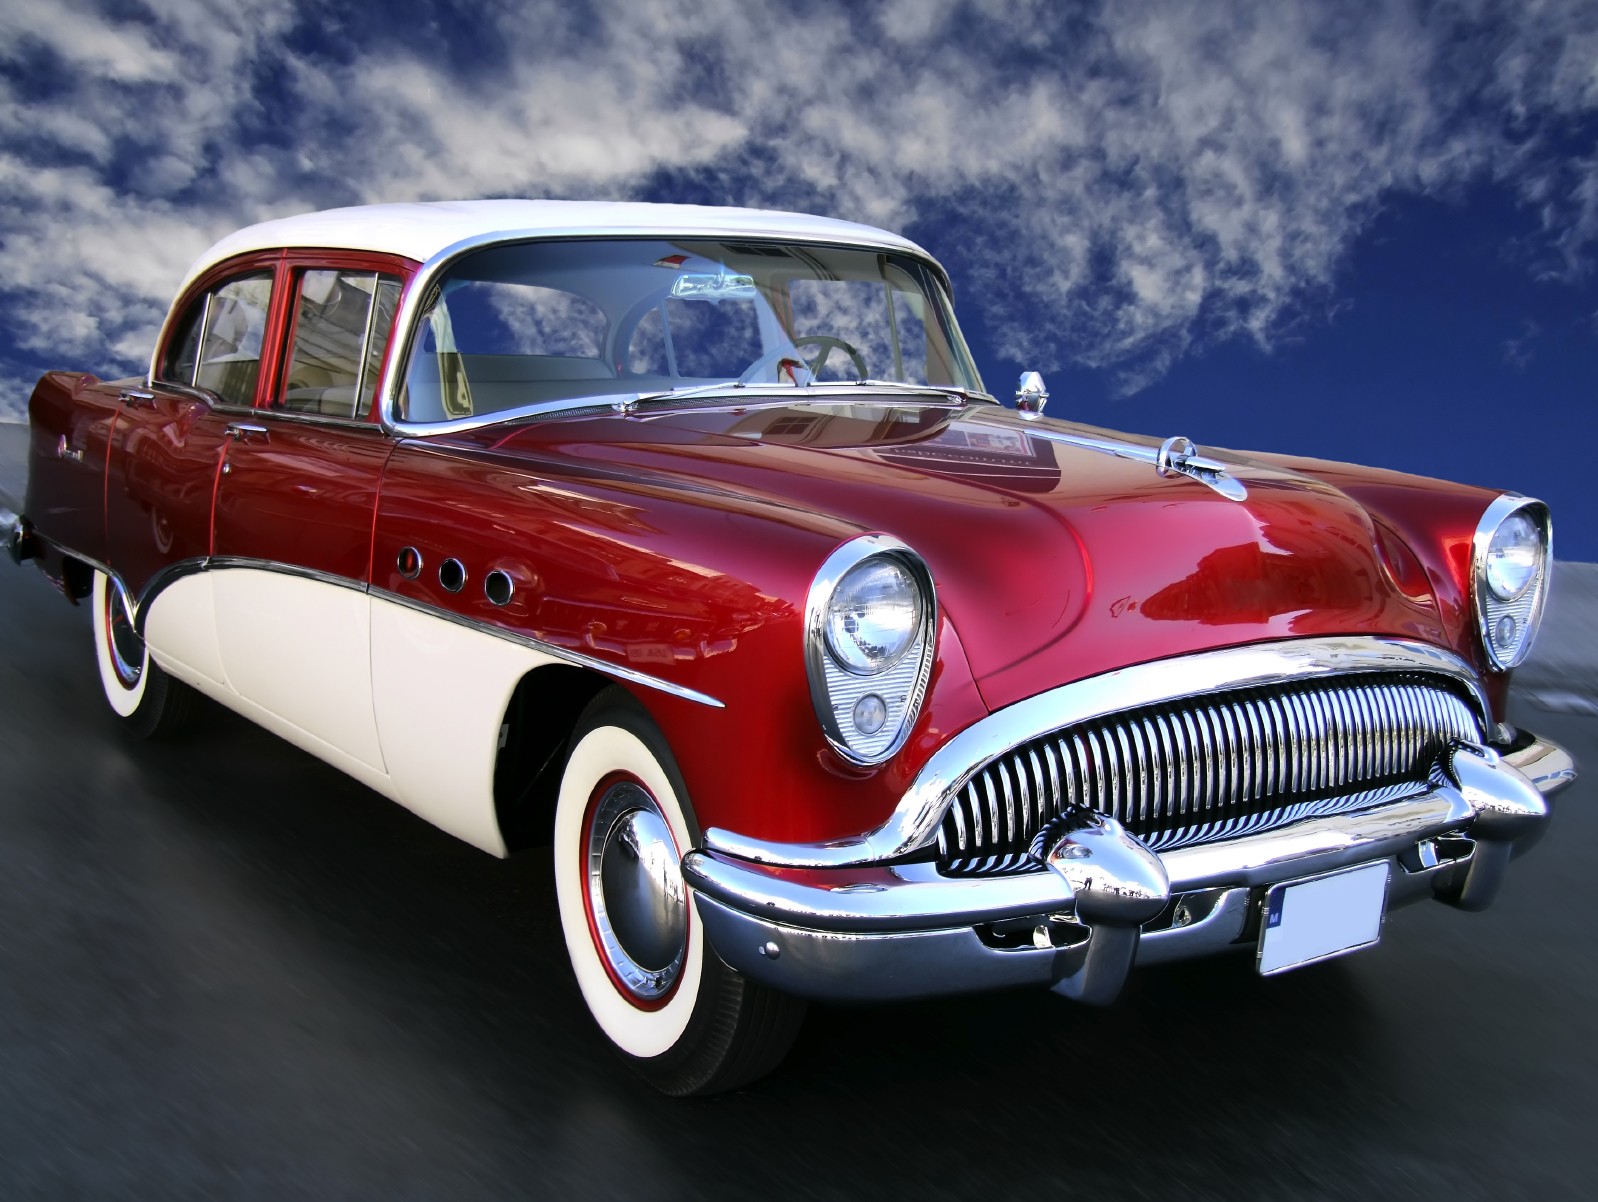
\includegraphics[width=\linewidth]{car.jpg} % regular UST num.2
	\end{subfigure}
	\begin{subfigure}[b]{0.225\linewidth}
		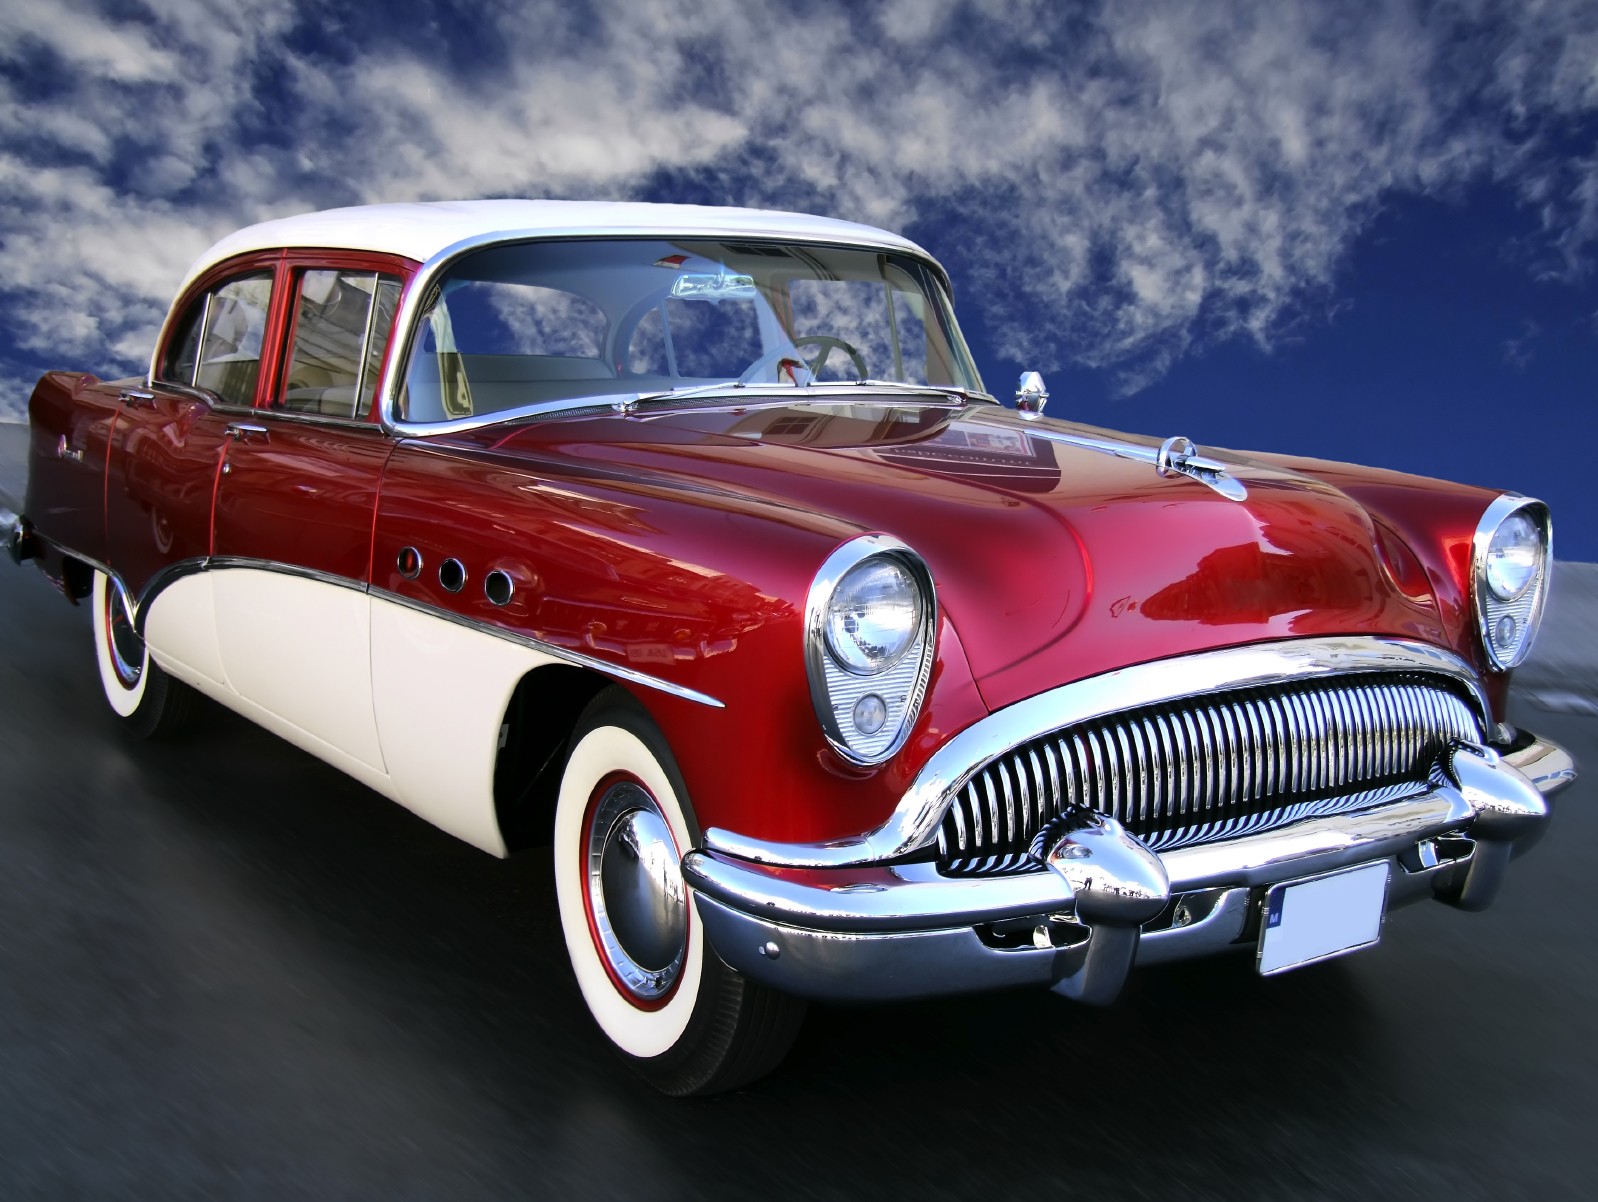
\includegraphics[width=\linewidth]{car.jpg} % UST+boos num.2
	\end{subfigure}
	% third line
	\centering
	\begin{subfigure}[b]{0.225\linewidth}
		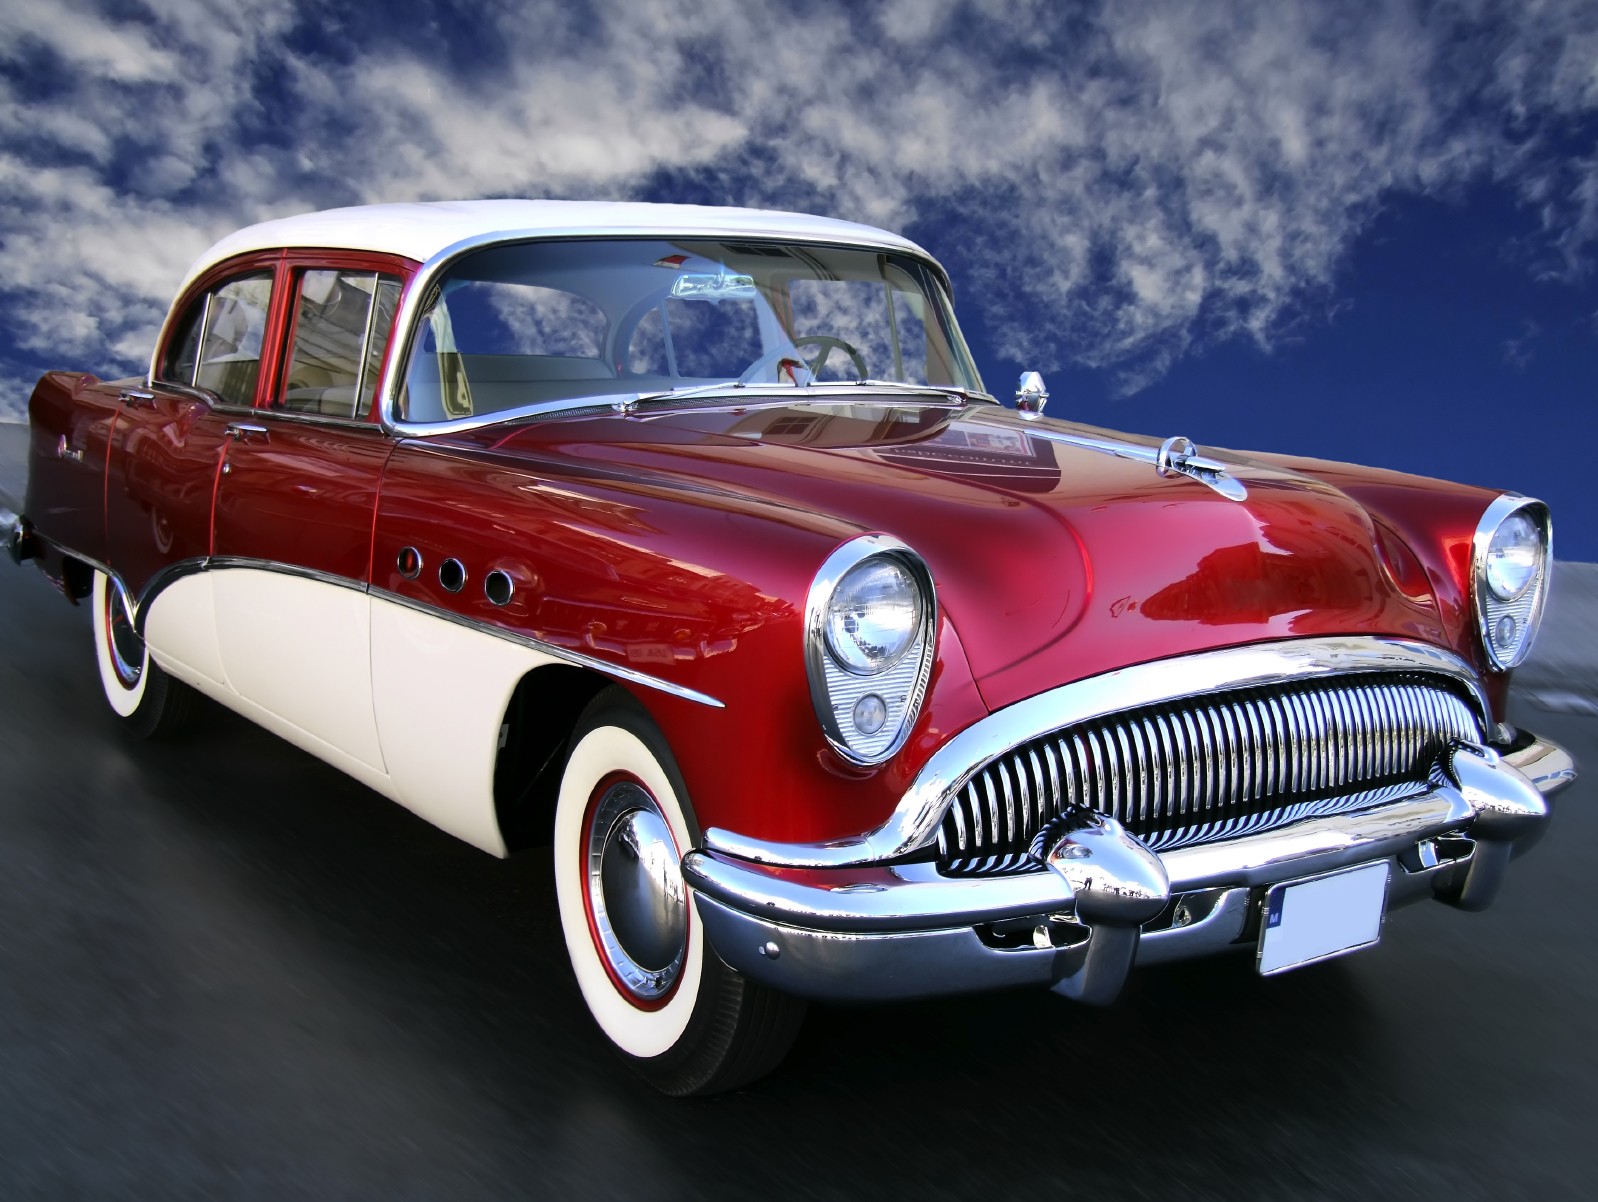
\includegraphics[width=\linewidth]{car.jpg} %style img num.3
		\caption{Style}
	\end{subfigure}
	\begin{subfigure}[b]{0.225\linewidth}
		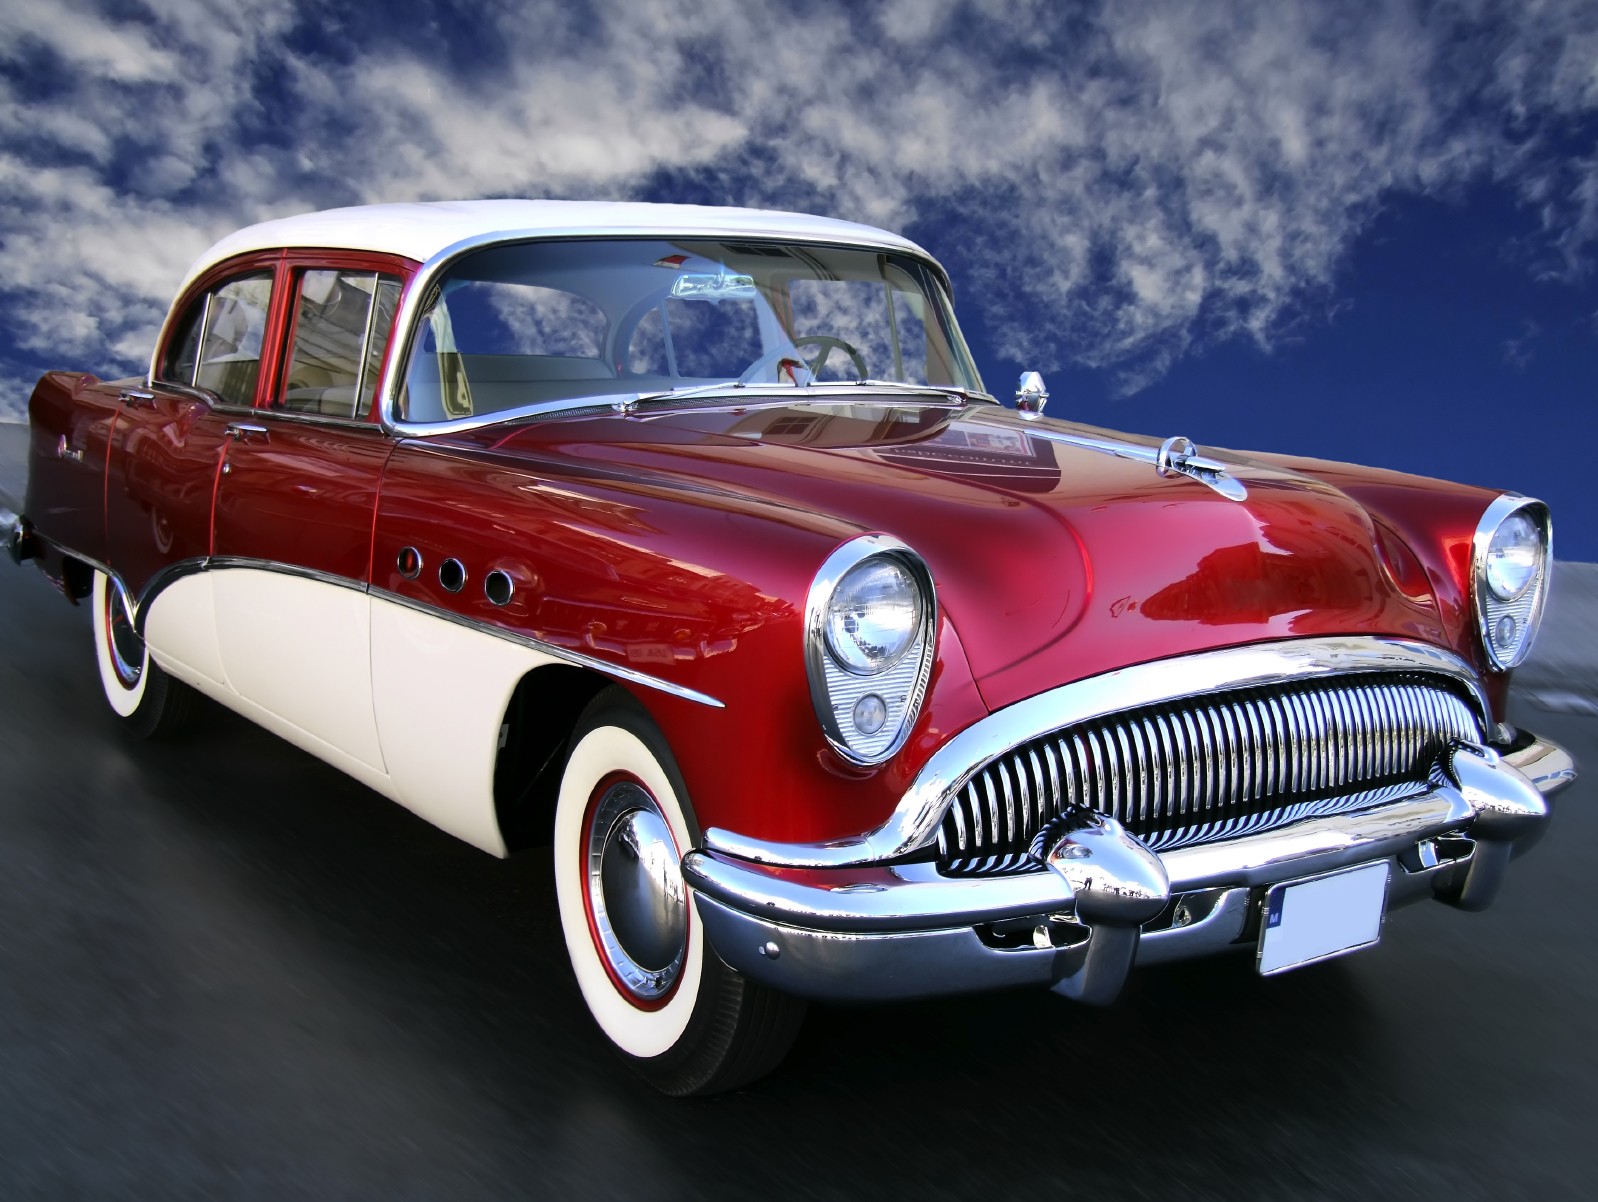
\includegraphics[width=\linewidth]{car.jpg} % content img num.3
		\caption{Content}
	\end{subfigure}
	\begin{subfigure}[b]{0.225\linewidth}
		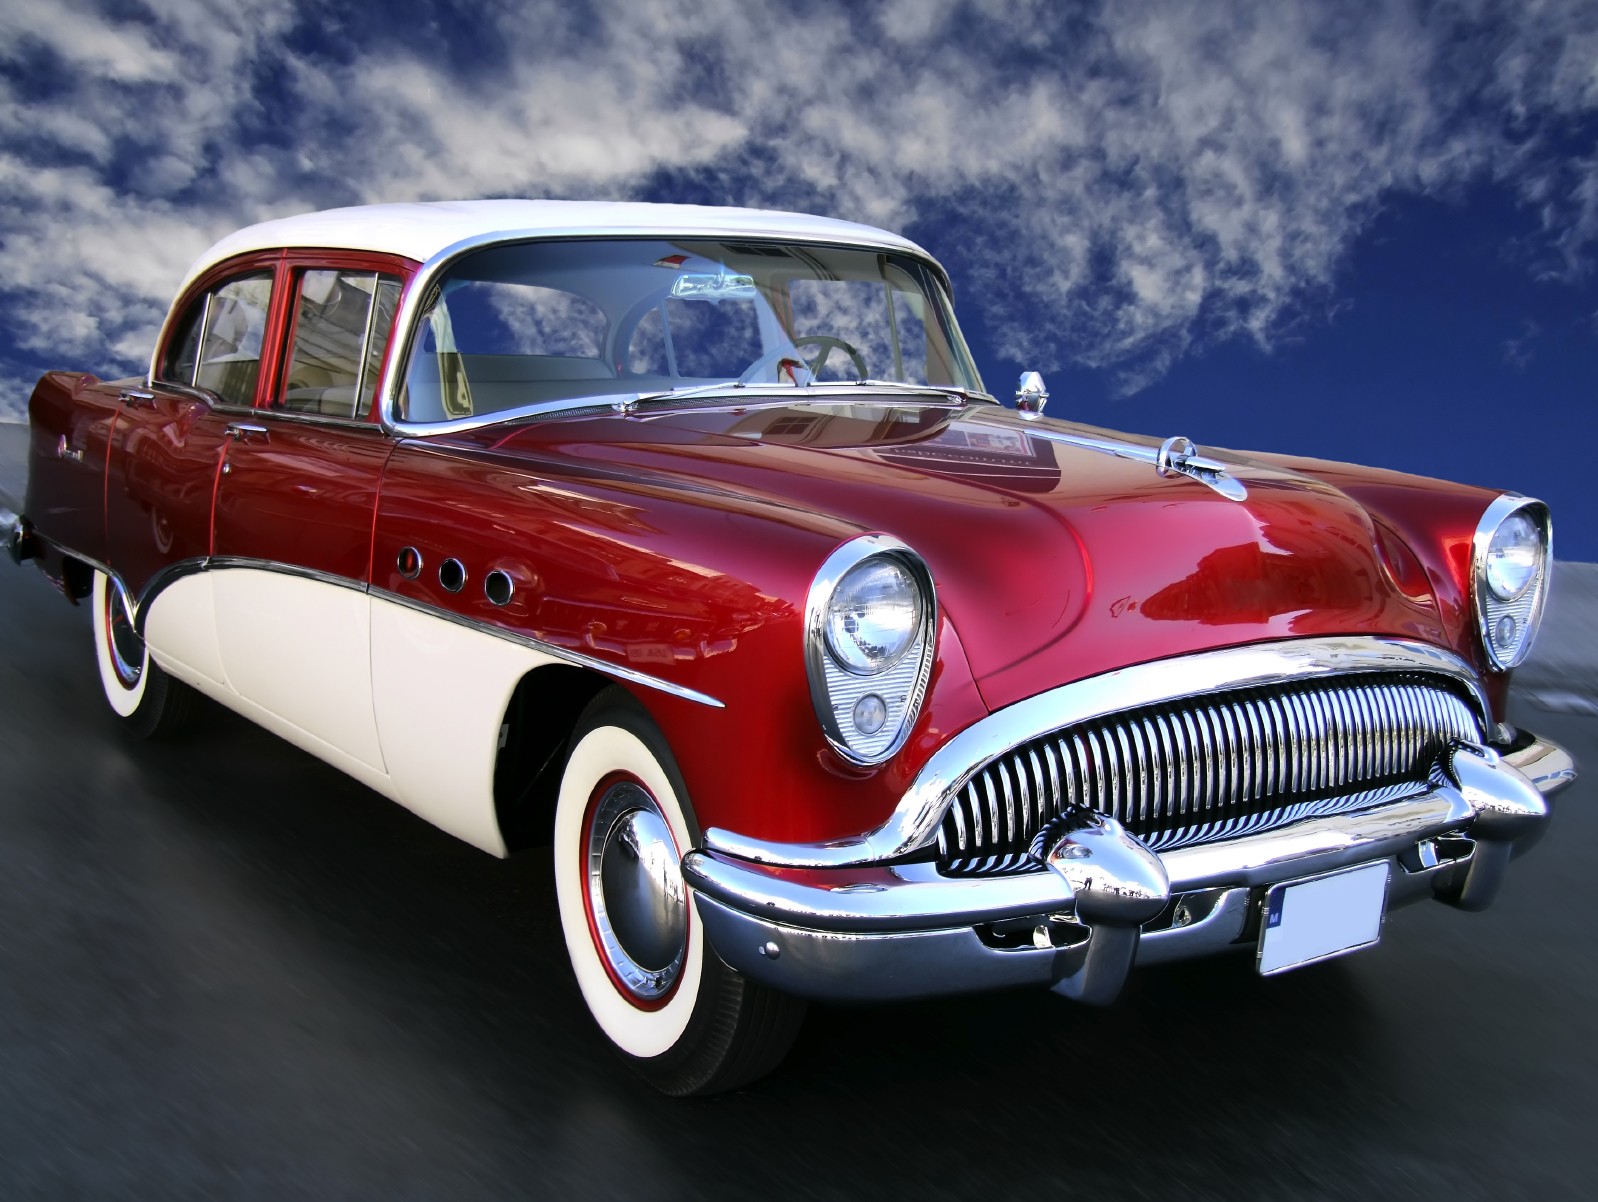
\includegraphics[width=\linewidth]{car.jpg} % regular UST num.3
		\caption{UST-Li et al. \cite{bib11}}
	\end{subfigure}
	\begin{subfigure}[b]{0.225\linewidth}
		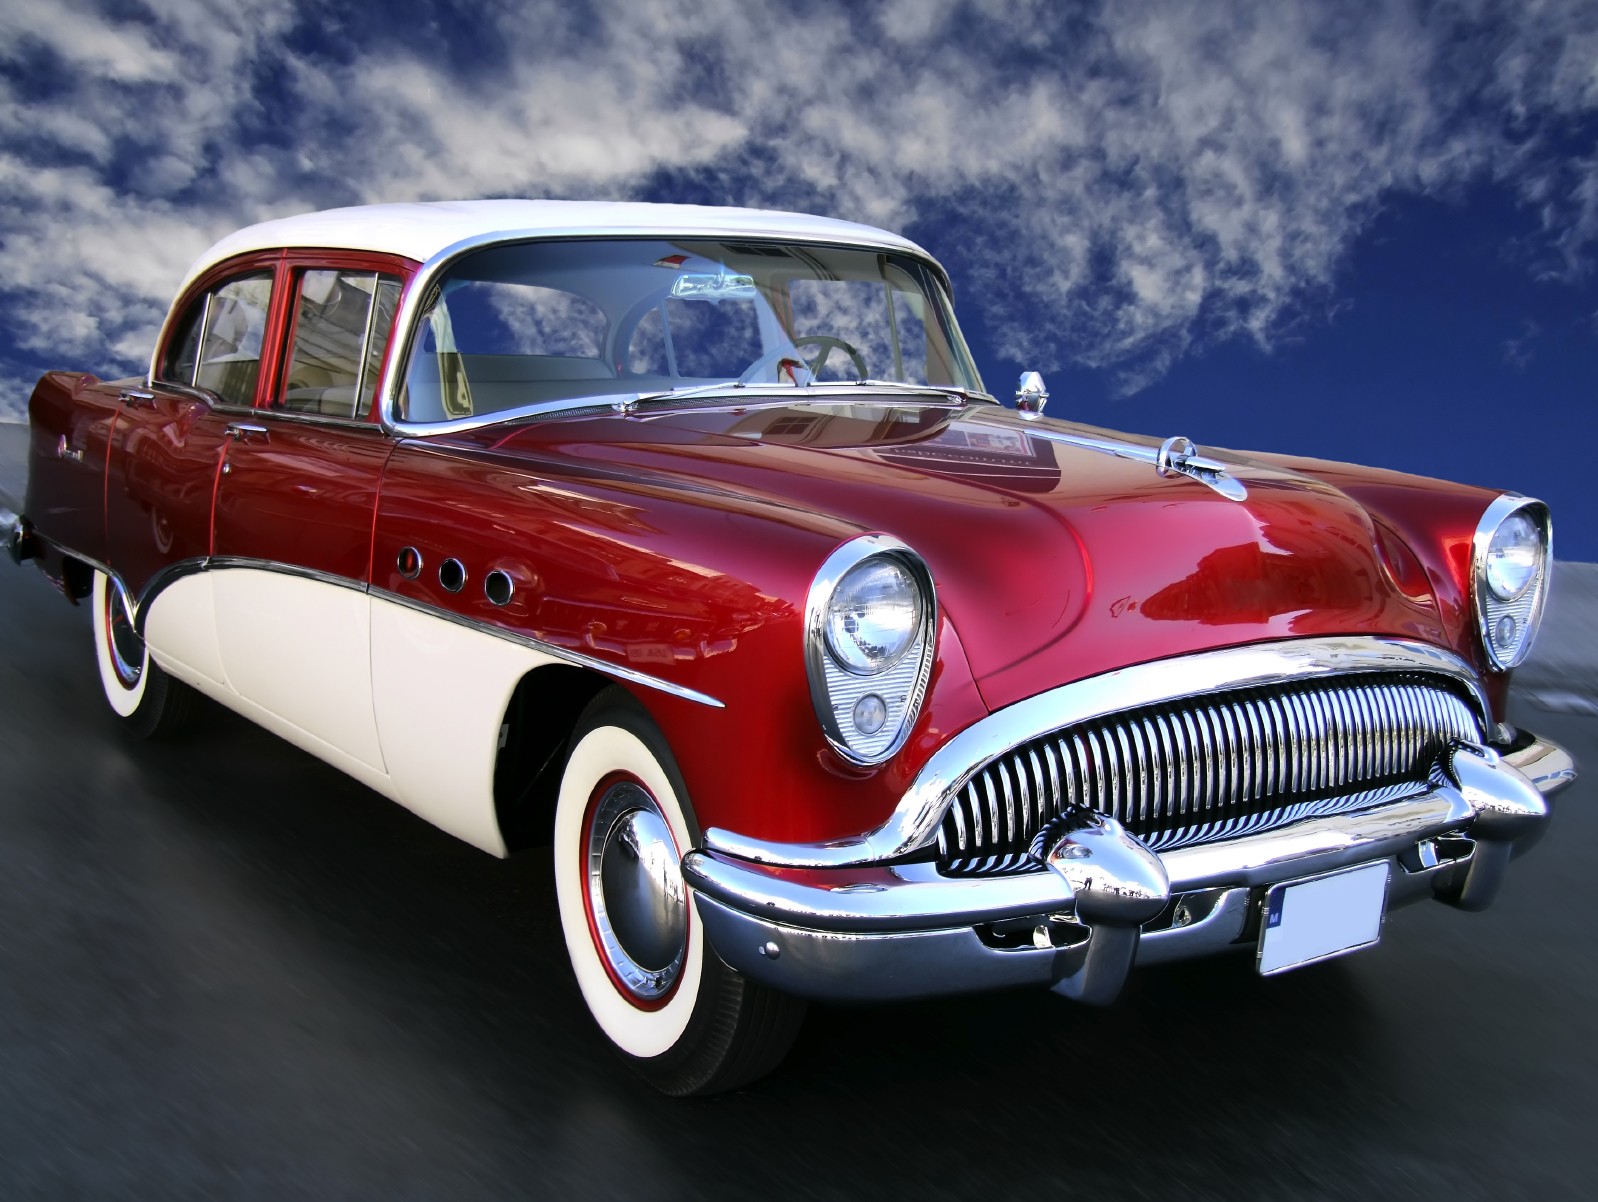
\includegraphics[width=\linewidth]{car.jpg} % UST+boos num.3
		\caption{UST+Boost}
	\end{subfigure}
	\caption{Results using Li et al. \cite{bib11} Encoder-Decoder architecture of UST, comparing our proposed method to boost stylization with the one Li et al. presented in \cite{bib11}.}
	\label{fig:Boost}
\end{figure}
% Merge  %
\subsubsection{Two styles merging methods}
\begin{figure}[h!]
	% first line
	\centering
	\begin{subfigure}[b]{0.13\linewidth}
		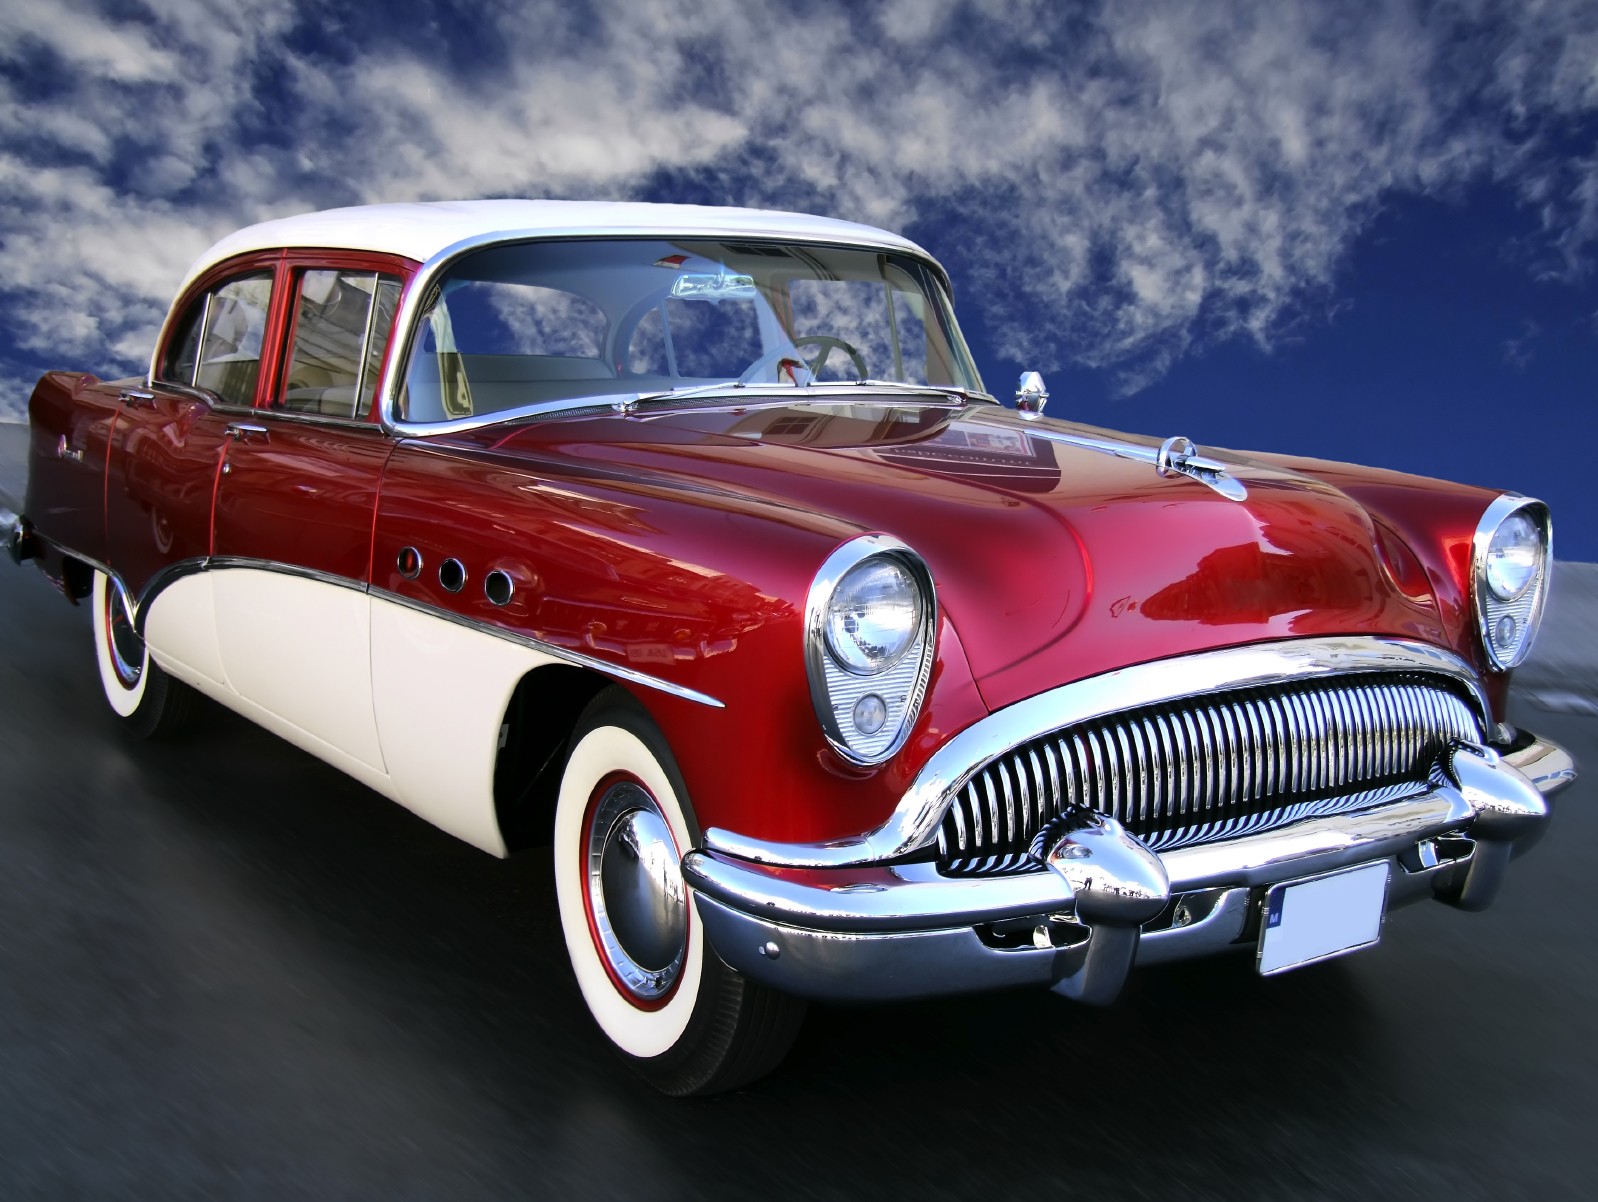
\includegraphics[width=\linewidth]{car.jpg} %style img num.1
	\end{subfigure}
	\begin{subfigure}[b]{0.13\linewidth}
		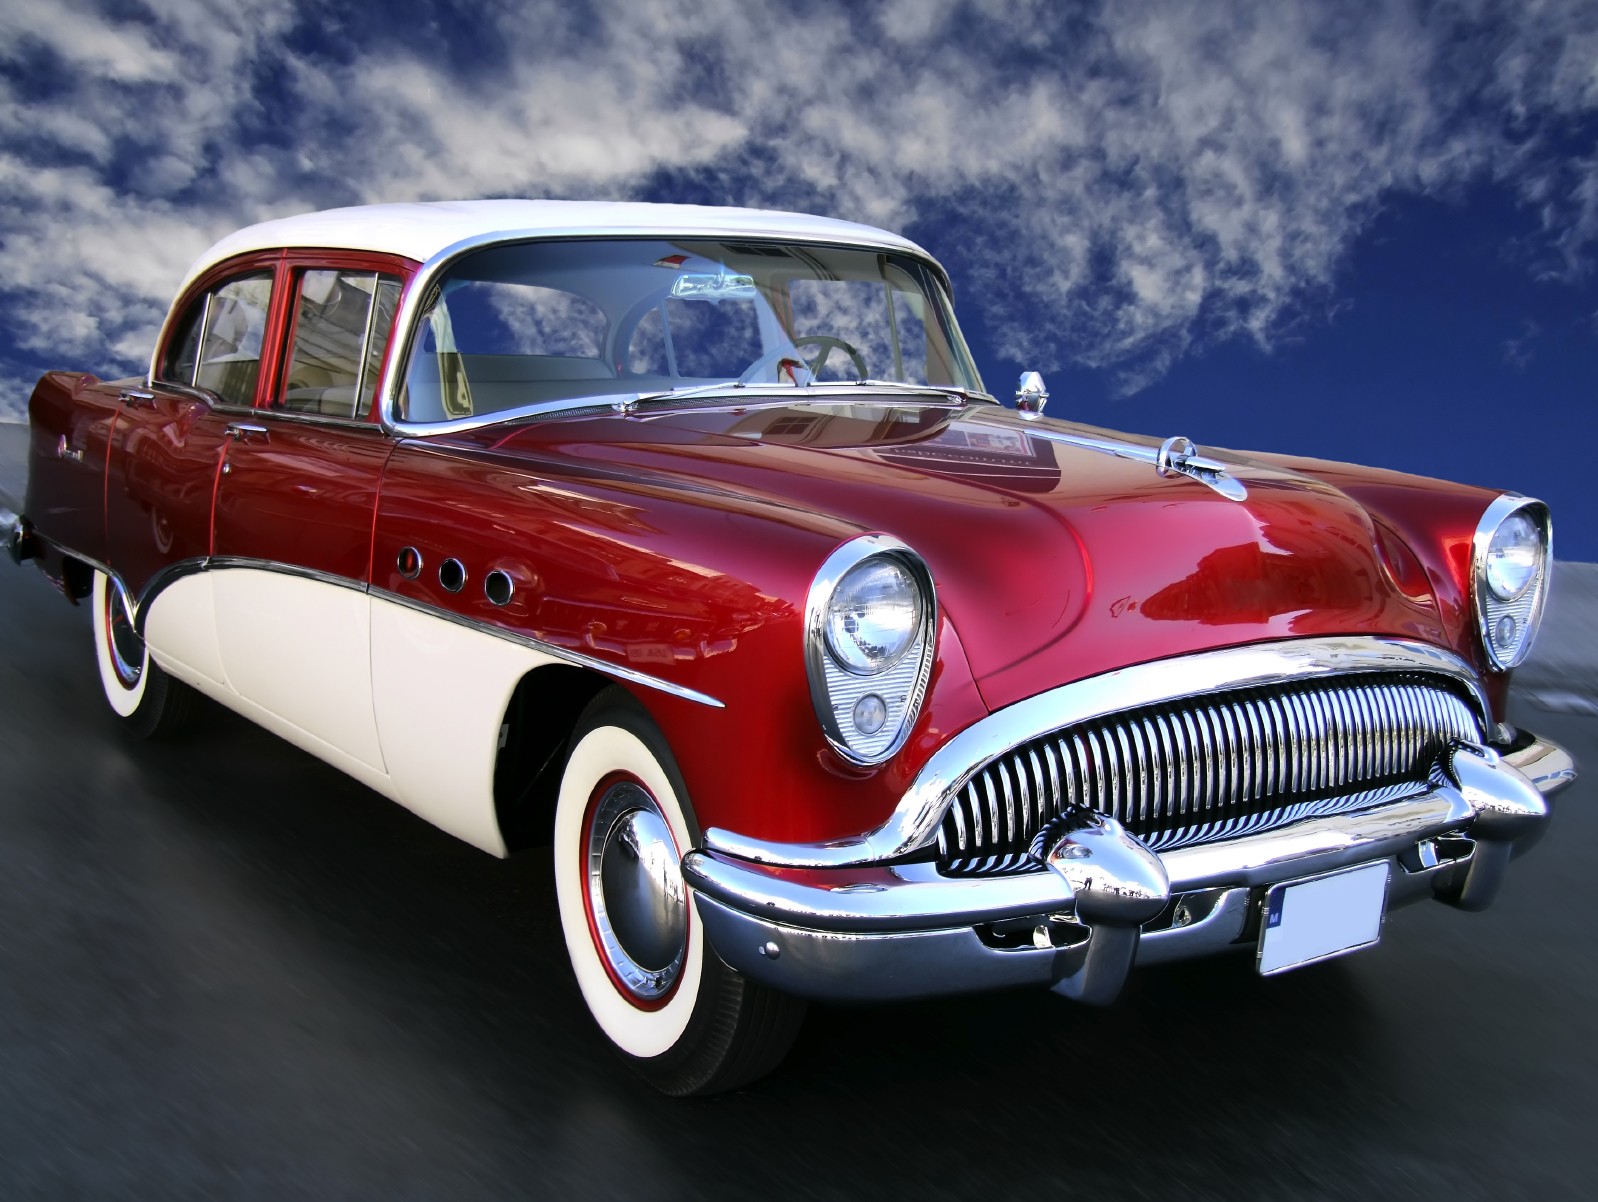
\includegraphics[width=\linewidth]{car.jpg} % style2 img num.1
	\end{subfigure}
	\begin{subfigure}[b]{0.13\linewidth}
		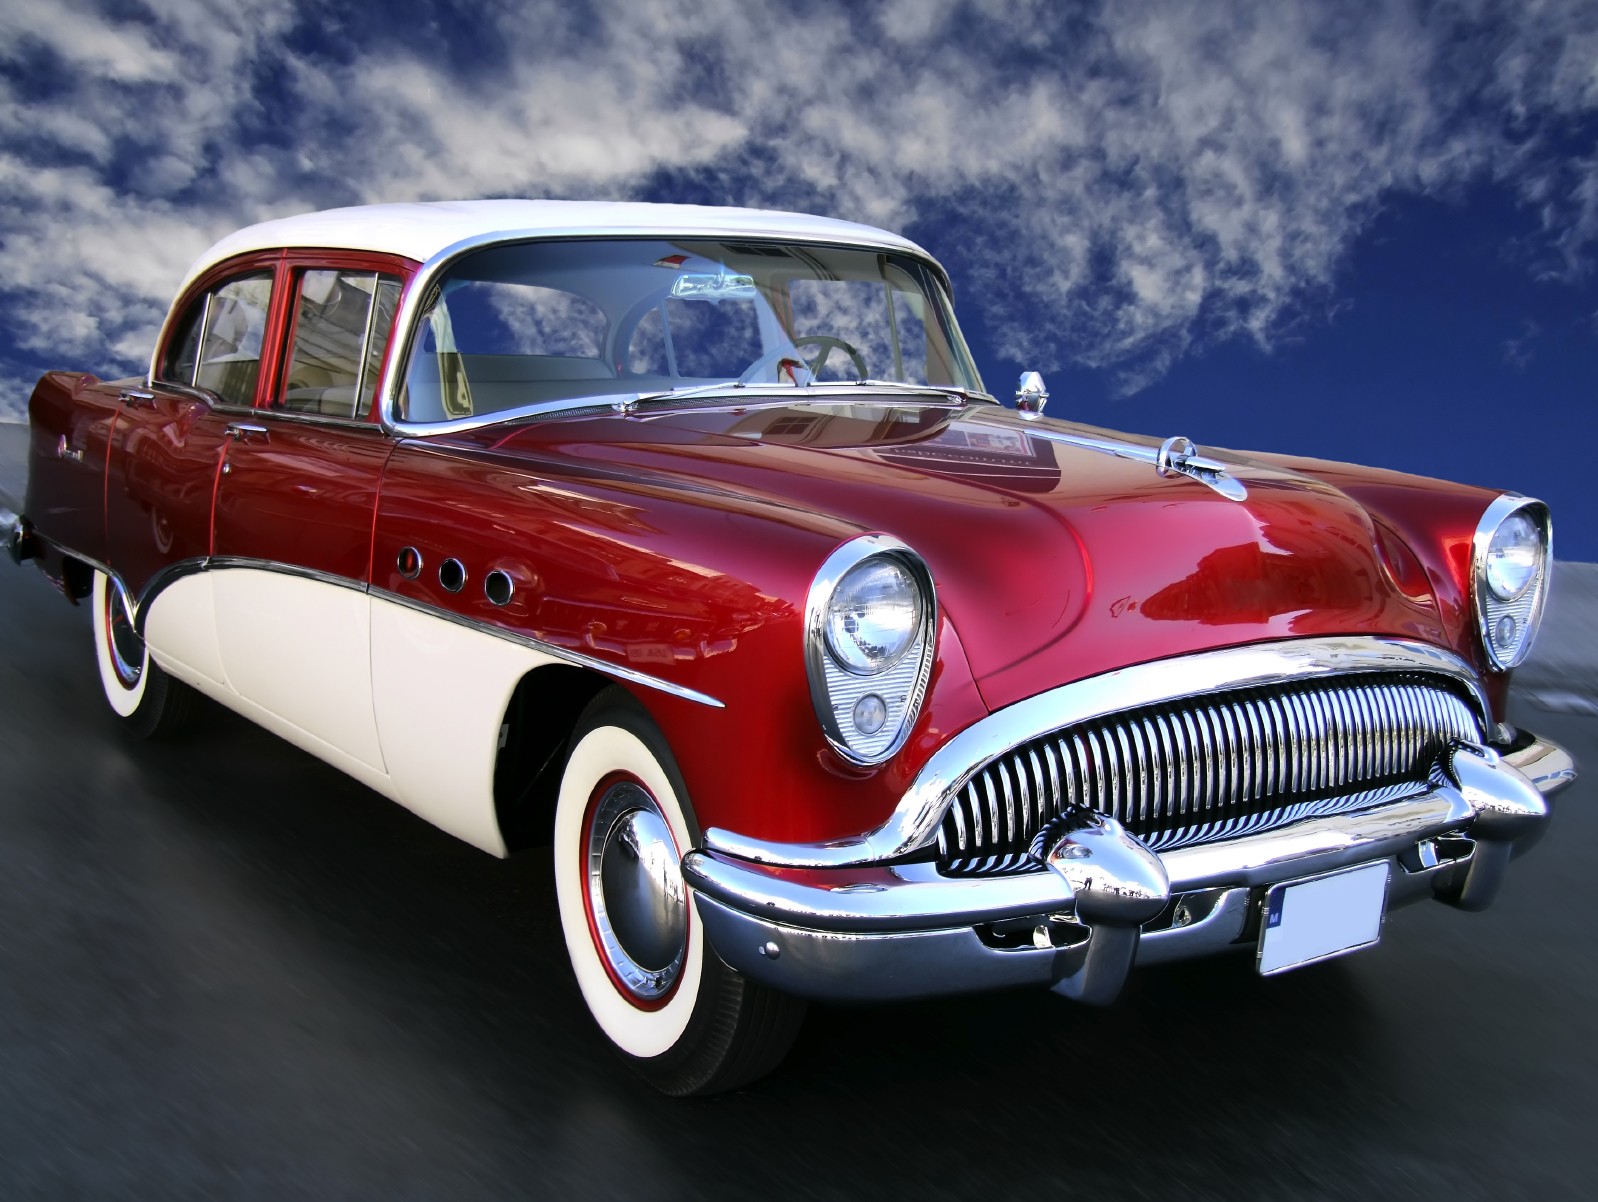
\includegraphics[width=\linewidth]{car.jpg} % content img num.1
	\end{subfigure}
	\begin{subfigure}[b]{0.13\linewidth}
		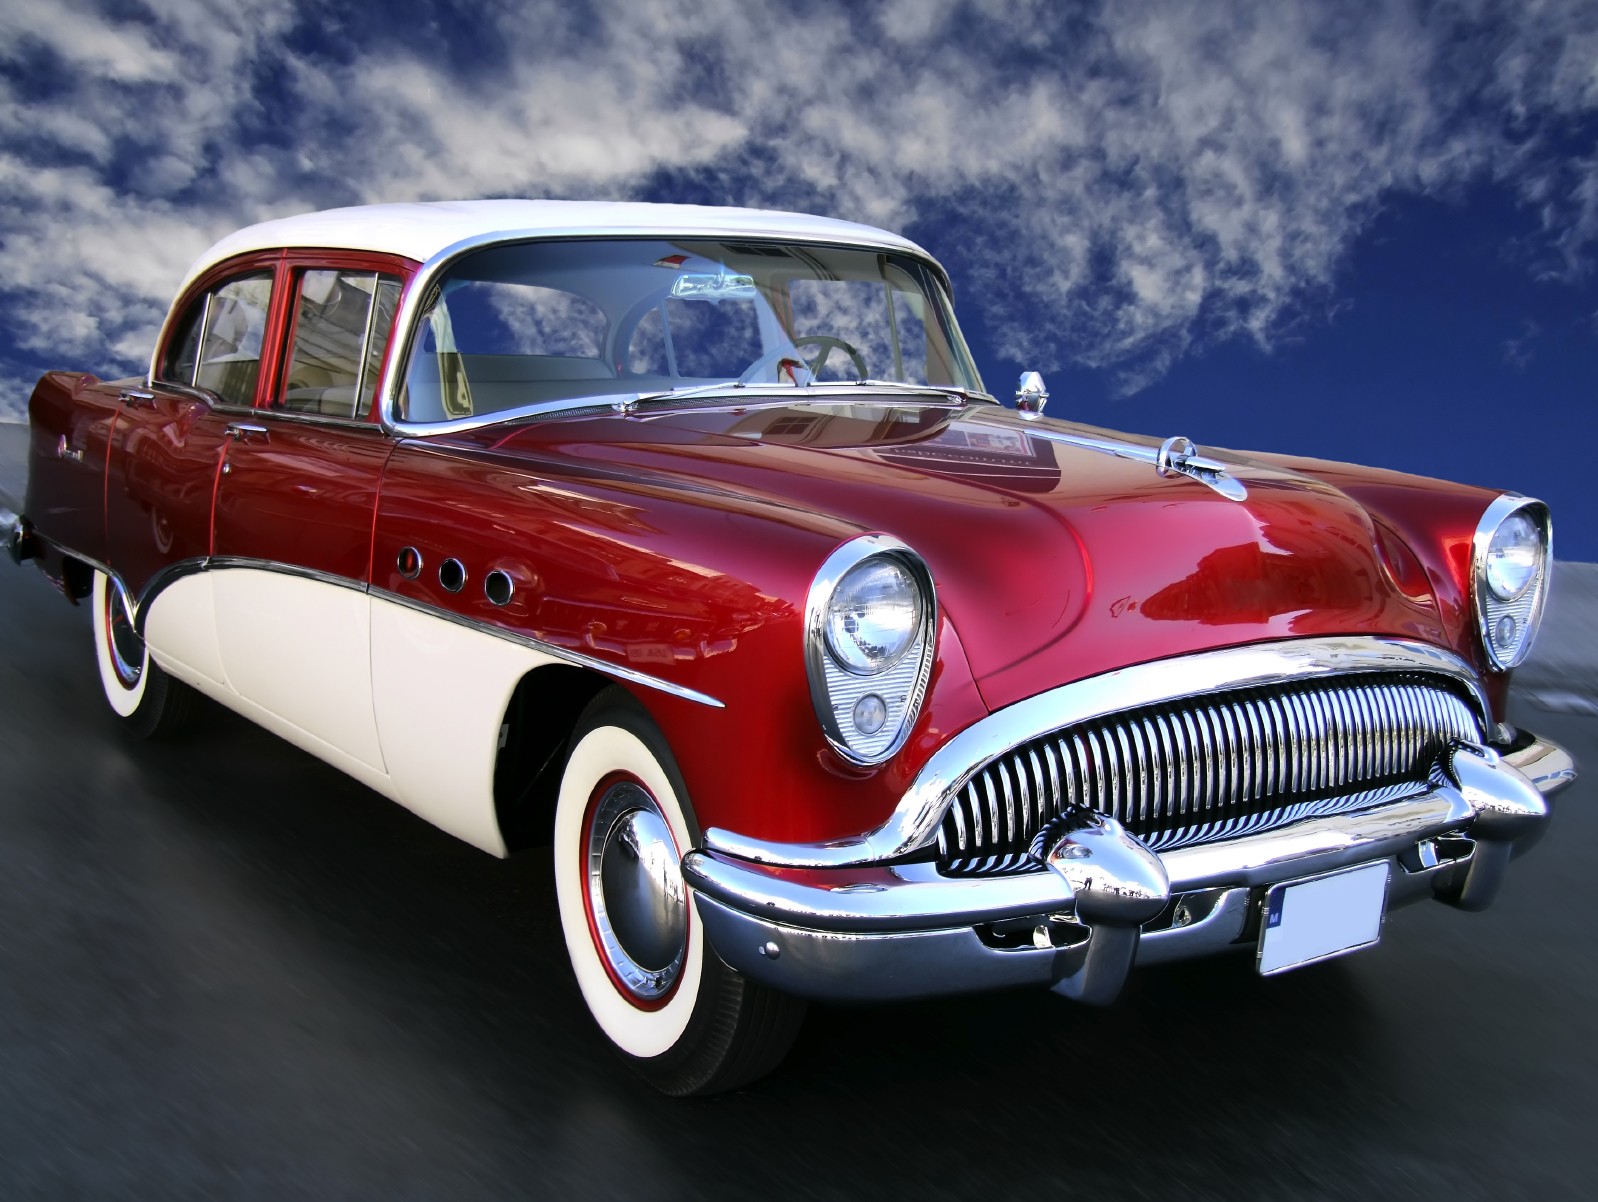
\includegraphics[width=\linewidth]{car.jpg} % orig merge num.1
	\end{subfigure}
	\begin{subfigure}[b]{0.13\linewidth}
		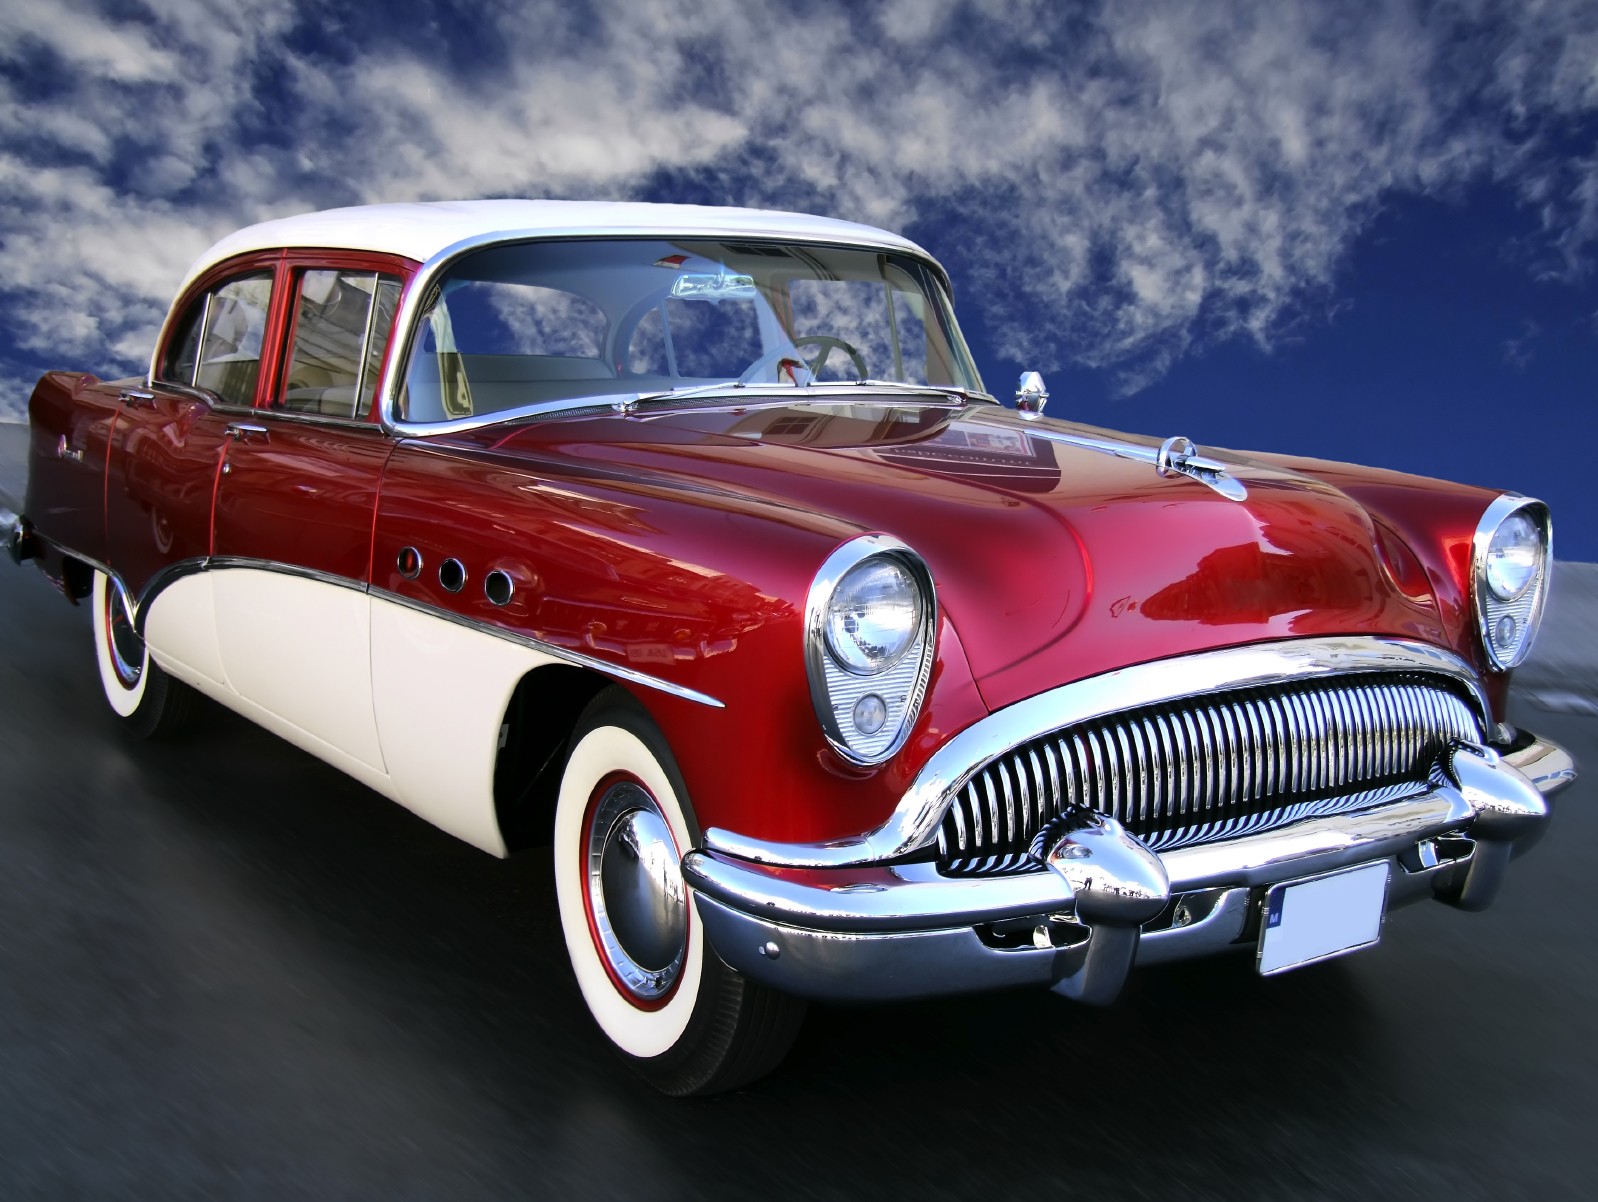
\includegraphics[width=\linewidth]{car.jpg} % merge1 num.1
	\end{subfigure}
	\begin{subfigure}[b]{0.13\linewidth}
		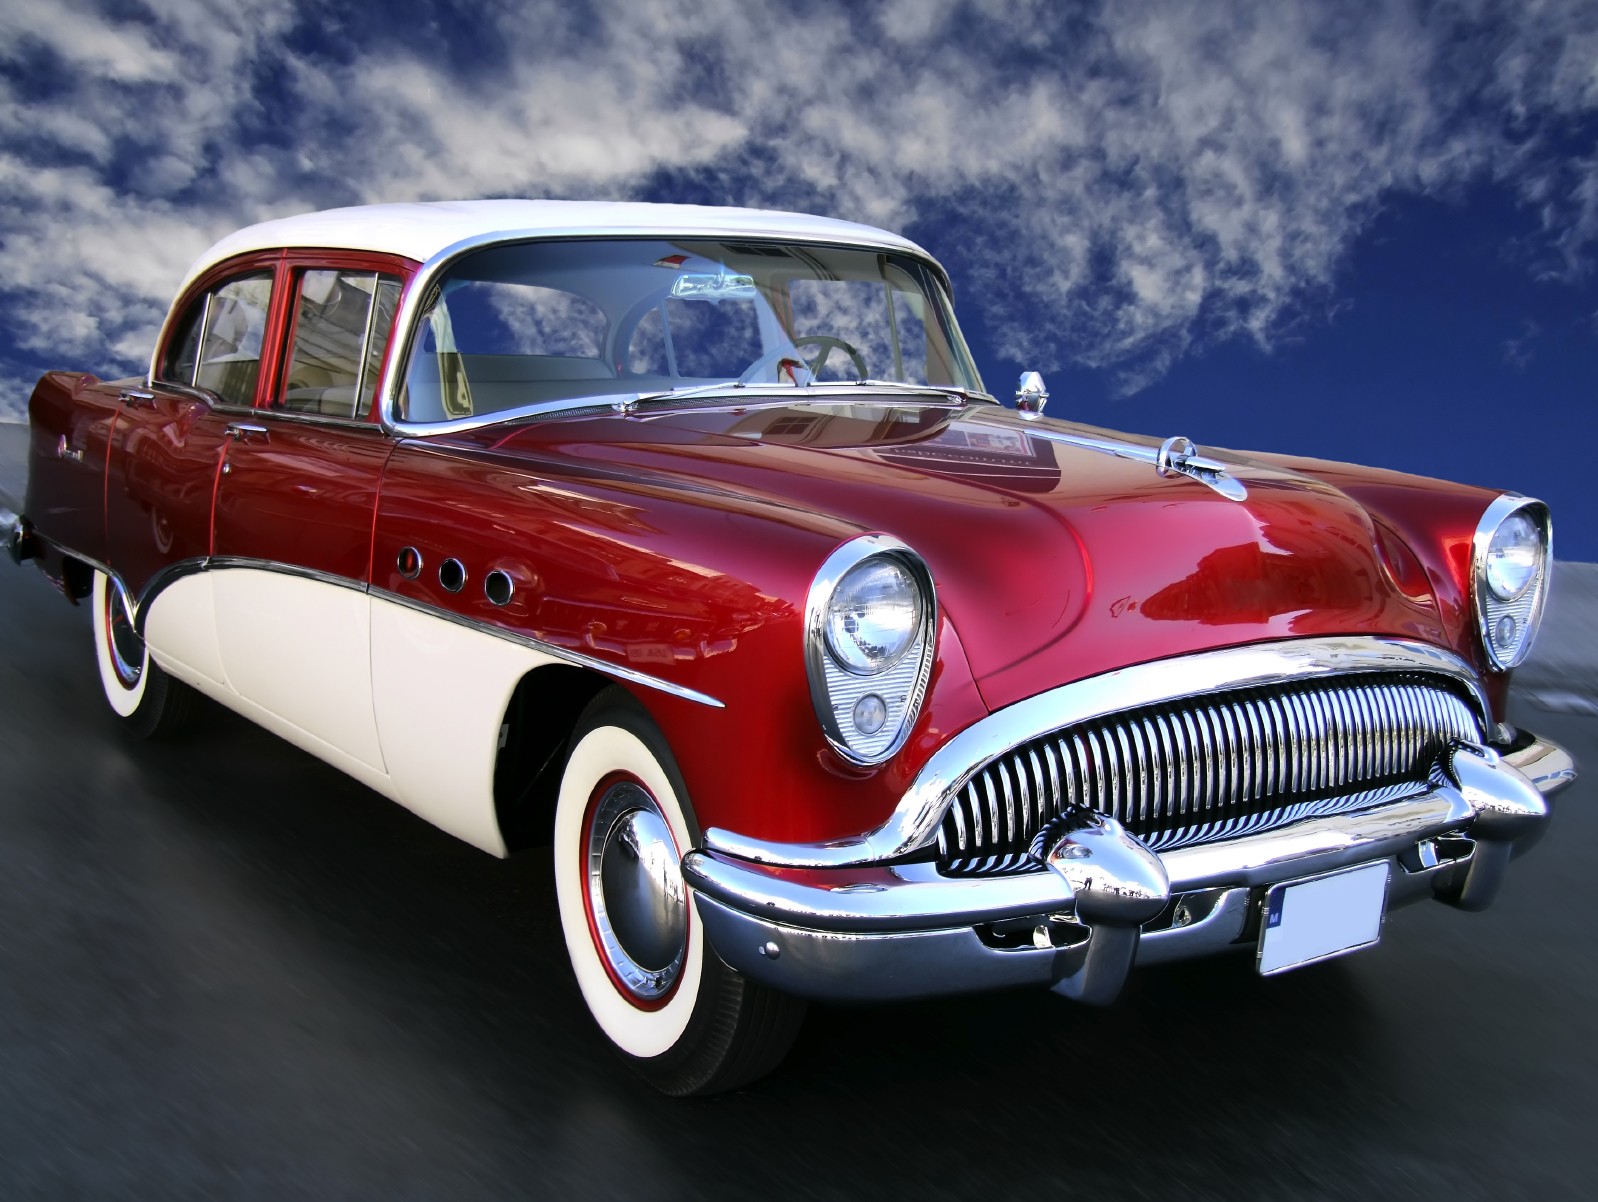
\includegraphics[width=\linewidth]{car.jpg} % merge2 num.1
	\end{subfigure}
	\begin{subfigure}[b]{0.13\linewidth}
		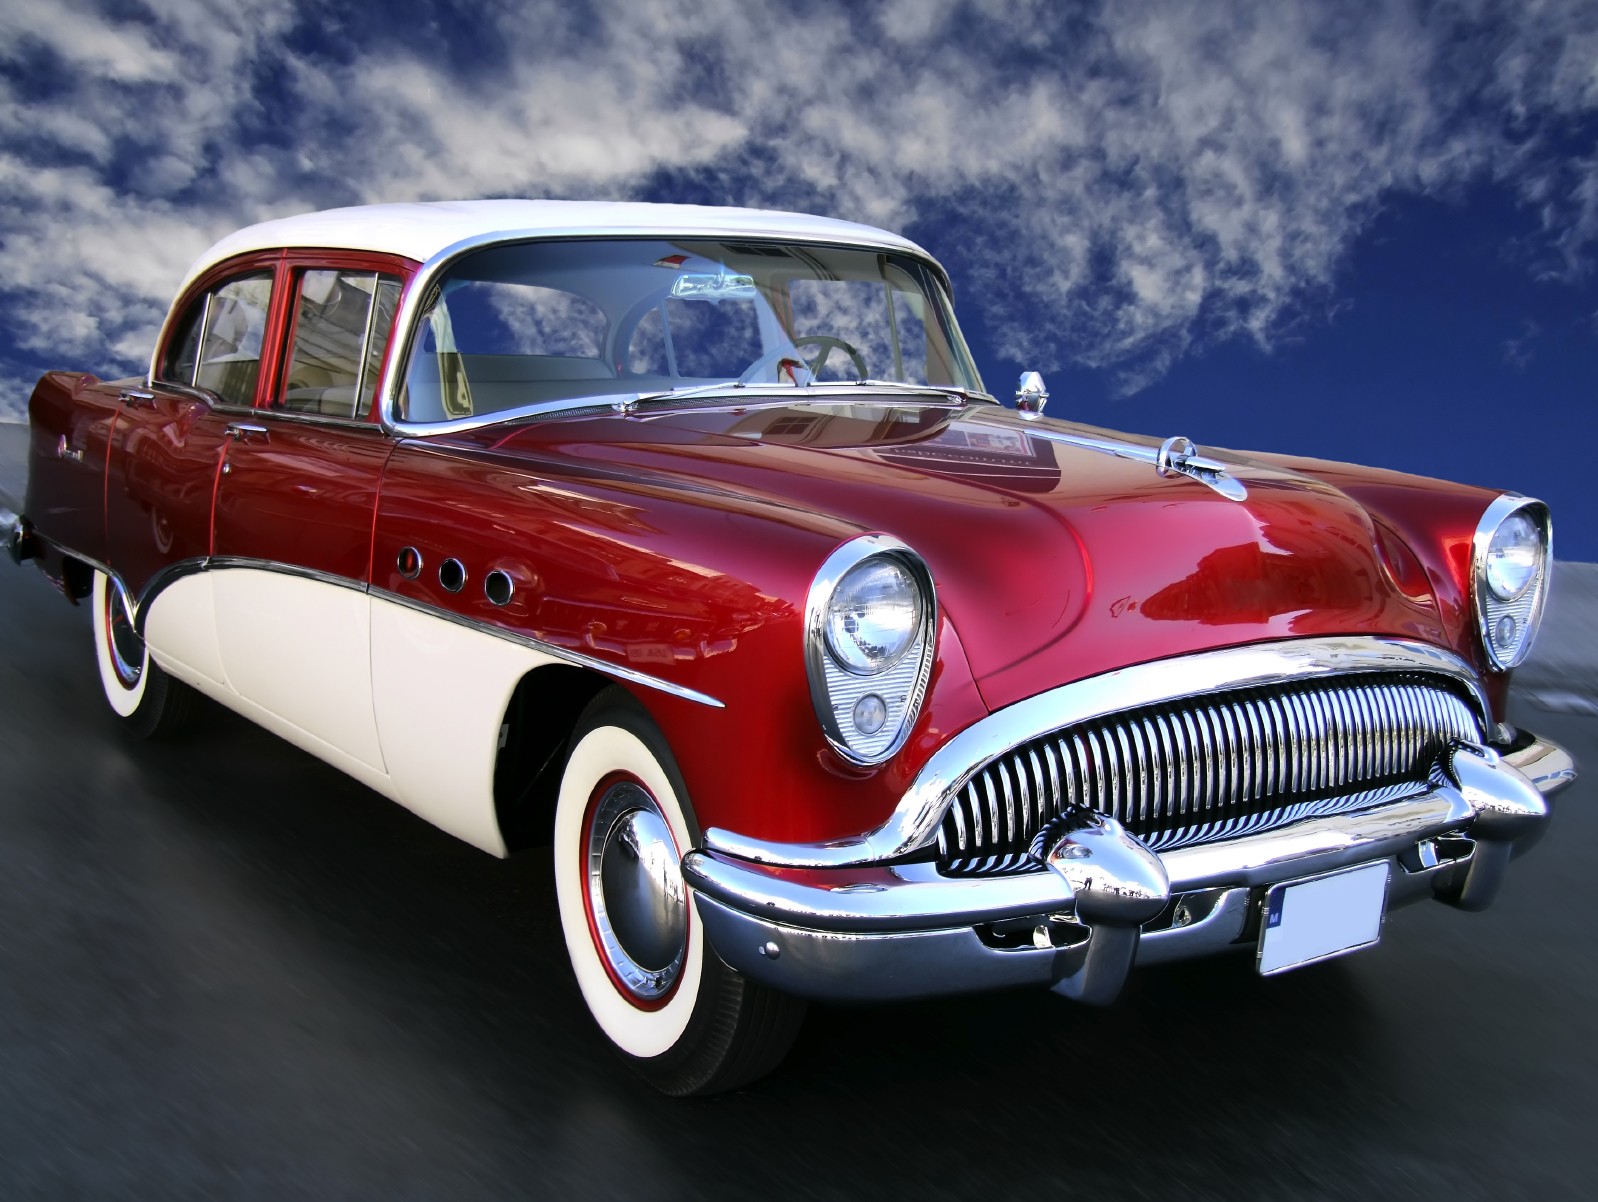
\includegraphics[width=\linewidth]{car.jpg} % merge3 num.1
	\end{subfigure}
	% second line
	\centering
	\begin{subfigure}[b]{0.13\linewidth}
		\includegraphics[width=\linewidth]{car.jpg} %style img num.2
	\end{subfigure}
	\begin{subfigure}[b]{0.13\linewidth}
		\includegraphics[width=\linewidth]{car.jpg} % style2 img num.2
	\end{subfigure}
	\begin{subfigure}[b]{0.13\linewidth}
		\includegraphics[width=\linewidth]{car.jpg} % content img num.2
	\end{subfigure}
	\begin{subfigure}[b]{0.13\linewidth}
		\includegraphics[width=\linewidth]{car.jpg} % orig merge num.2
	\end{subfigure}
	\begin{subfigure}[b]{0.13\linewidth}
		\includegraphics[width=\linewidth]{car.jpg} % merge1 num.2
	\end{subfigure}
	\begin{subfigure}[b]{0.13\linewidth}
		\includegraphics[width=\linewidth]{car.jpg} % merge2 num.2
	\end{subfigure}
	\begin{subfigure}[b]{0.13\linewidth}
		\includegraphics[width=\linewidth]{car.jpg} % merge3 num.2
	\end{subfigure}
	% third line
	\centering
	\begin{subfigure}[b]{0.13\linewidth}
		\includegraphics[width=\linewidth]{car.jpg} %style img num.3
		\caption{$1_{st}$ \\ Style}
	\end{subfigure}
	\begin{subfigure}[b]{0.13\linewidth}
		\includegraphics[width=\linewidth]{car.jpg} %style2 img num.3
		\caption{$2_{nd}$ \\ Style}
	\end{subfigure}
	\begin{subfigure}[b]{0.13\linewidth}
		\includegraphics[width=\linewidth]{car.jpg} % content img num.3
		\caption{Content \\ image}
	\end{subfigure}
	\begin{subfigure}[b]{0.13\linewidth}
		\includegraphics[width=\linewidth]{car.jpg} % orig merge num.3
		\caption{Li et al. \cite{bib11}}
	\end{subfigure}
	\begin{subfigure}[b]{0.13\linewidth}
		\includegraphics[width=\linewidth]{car.jpg} % merge1 num.3
		\caption{$1_{st}$ method}
	\end{subfigure}
	\begin{subfigure}[b]{0.13\linewidth}
		\includegraphics[width=\linewidth]{car.jpg} % merge2 num.3
		\caption{$2_{nd}$ method}
	\end{subfigure}
	\begin{subfigure}[b]{0.13\linewidth}
		\includegraphics[width=\linewidth]{car.jpg} % merge3 num.3
		\caption{$3_{rd}$ method}
	\end{subfigure}
		\caption{Results using different stylization methods. (d) is the original merge method as in \cite{bib11}, (e) is Level Merge, (f) is Channel Merge and (g) is Interpolate-Style Merge.}
		\label{fig:Merge}
\end{figure}
add more text here
add texture synthesis 